% Options for packages loaded elsewhere
\PassOptionsToPackage{unicode}{hyperref}
\PassOptionsToPackage{hyphens}{url}
\PassOptionsToPackage{dvipsnames,svgnames,x11names}{xcolor}
%
\documentclass[
  letterpaper,
  DIV=11,
  numbers=noendperiod]{scrartcl}

\usepackage{amsmath,amssymb}
\usepackage{iftex}
\ifPDFTeX
  \usepackage[T1]{fontenc}
  \usepackage[utf8]{inputenc}
  \usepackage{textcomp} % provide euro and other symbols
\else % if luatex or xetex
  \usepackage{unicode-math}
  \defaultfontfeatures{Scale=MatchLowercase}
  \defaultfontfeatures[\rmfamily]{Ligatures=TeX,Scale=1}
\fi
\usepackage{lmodern}
\ifPDFTeX\else  
    % xetex/luatex font selection
  \setmainfont[]{Open Sans}
\fi
% Use upquote if available, for straight quotes in verbatim environments
\IfFileExists{upquote.sty}{\usepackage{upquote}}{}
\IfFileExists{microtype.sty}{% use microtype if available
  \usepackage[]{microtype}
  \UseMicrotypeSet[protrusion]{basicmath} % disable protrusion for tt fonts
}{}
\makeatletter
\@ifundefined{KOMAClassName}{% if non-KOMA class
  \IfFileExists{parskip.sty}{%
    \usepackage{parskip}
  }{% else
    \setlength{\parindent}{0pt}
    \setlength{\parskip}{6pt plus 2pt minus 1pt}}
}{% if KOMA class
  \KOMAoptions{parskip=half}}
\makeatother
\usepackage{xcolor}
\setlength{\emergencystretch}{3em} % prevent overfull lines
\setcounter{secnumdepth}{-\maxdimen} % remove section numbering
% Make \paragraph and \subparagraph free-standing
\ifx\paragraph\undefined\else
  \let\oldparagraph\paragraph
  \renewcommand{\paragraph}[1]{\oldparagraph{#1}\mbox{}}
\fi
\ifx\subparagraph\undefined\else
  \let\oldsubparagraph\subparagraph
  \renewcommand{\subparagraph}[1]{\oldsubparagraph{#1}\mbox{}}
\fi

\usepackage{color}
\usepackage{fancyvrb}
\newcommand{\VerbBar}{|}
\newcommand{\VERB}{\Verb[commandchars=\\\{\}]}
\DefineVerbatimEnvironment{Highlighting}{Verbatim}{commandchars=\\\{\}}
% Add ',fontsize=\small' for more characters per line
\usepackage{framed}
\definecolor{shadecolor}{RGB}{241,243,245}
\newenvironment{Shaded}{\begin{snugshade}}{\end{snugshade}}
\newcommand{\AlertTok}[1]{\textcolor[rgb]{0.68,0.00,0.00}{#1}}
\newcommand{\AnnotationTok}[1]{\textcolor[rgb]{0.37,0.37,0.37}{#1}}
\newcommand{\AttributeTok}[1]{\textcolor[rgb]{0.40,0.45,0.13}{#1}}
\newcommand{\BaseNTok}[1]{\textcolor[rgb]{0.68,0.00,0.00}{#1}}
\newcommand{\BuiltInTok}[1]{\textcolor[rgb]{0.00,0.23,0.31}{#1}}
\newcommand{\CharTok}[1]{\textcolor[rgb]{0.13,0.47,0.30}{#1}}
\newcommand{\CommentTok}[1]{\textcolor[rgb]{0.37,0.37,0.37}{#1}}
\newcommand{\CommentVarTok}[1]{\textcolor[rgb]{0.37,0.37,0.37}{\textit{#1}}}
\newcommand{\ConstantTok}[1]{\textcolor[rgb]{0.56,0.35,0.01}{#1}}
\newcommand{\ControlFlowTok}[1]{\textcolor[rgb]{0.00,0.23,0.31}{#1}}
\newcommand{\DataTypeTok}[1]{\textcolor[rgb]{0.68,0.00,0.00}{#1}}
\newcommand{\DecValTok}[1]{\textcolor[rgb]{0.68,0.00,0.00}{#1}}
\newcommand{\DocumentationTok}[1]{\textcolor[rgb]{0.37,0.37,0.37}{\textit{#1}}}
\newcommand{\ErrorTok}[1]{\textcolor[rgb]{0.68,0.00,0.00}{#1}}
\newcommand{\ExtensionTok}[1]{\textcolor[rgb]{0.00,0.23,0.31}{#1}}
\newcommand{\FloatTok}[1]{\textcolor[rgb]{0.68,0.00,0.00}{#1}}
\newcommand{\FunctionTok}[1]{\textcolor[rgb]{0.28,0.35,0.67}{#1}}
\newcommand{\ImportTok}[1]{\textcolor[rgb]{0.00,0.46,0.62}{#1}}
\newcommand{\InformationTok}[1]{\textcolor[rgb]{0.37,0.37,0.37}{#1}}
\newcommand{\KeywordTok}[1]{\textcolor[rgb]{0.00,0.23,0.31}{#1}}
\newcommand{\NormalTok}[1]{\textcolor[rgb]{0.00,0.23,0.31}{#1}}
\newcommand{\OperatorTok}[1]{\textcolor[rgb]{0.37,0.37,0.37}{#1}}
\newcommand{\OtherTok}[1]{\textcolor[rgb]{0.00,0.23,0.31}{#1}}
\newcommand{\PreprocessorTok}[1]{\textcolor[rgb]{0.68,0.00,0.00}{#1}}
\newcommand{\RegionMarkerTok}[1]{\textcolor[rgb]{0.00,0.23,0.31}{#1}}
\newcommand{\SpecialCharTok}[1]{\textcolor[rgb]{0.37,0.37,0.37}{#1}}
\newcommand{\SpecialStringTok}[1]{\textcolor[rgb]{0.13,0.47,0.30}{#1}}
\newcommand{\StringTok}[1]{\textcolor[rgb]{0.13,0.47,0.30}{#1}}
\newcommand{\VariableTok}[1]{\textcolor[rgb]{0.07,0.07,0.07}{#1}}
\newcommand{\VerbatimStringTok}[1]{\textcolor[rgb]{0.13,0.47,0.30}{#1}}
\newcommand{\WarningTok}[1]{\textcolor[rgb]{0.37,0.37,0.37}{\textit{#1}}}

\providecommand{\tightlist}{%
  \setlength{\itemsep}{0pt}\setlength{\parskip}{0pt}}\usepackage{longtable,booktabs,array}
\usepackage{calc} % for calculating minipage widths
% Correct order of tables after \paragraph or \subparagraph
\usepackage{etoolbox}
\makeatletter
\patchcmd\longtable{\par}{\if@noskipsec\mbox{}\fi\par}{}{}
\makeatother
% Allow footnotes in longtable head/foot
\IfFileExists{footnotehyper.sty}{\usepackage{footnotehyper}}{\usepackage{footnote}}
\makesavenoteenv{longtable}
\usepackage{graphicx}
\makeatletter
\def\maxwidth{\ifdim\Gin@nat@width>\linewidth\linewidth\else\Gin@nat@width\fi}
\def\maxheight{\ifdim\Gin@nat@height>\textheight\textheight\else\Gin@nat@height\fi}
\makeatother
% Scale images if necessary, so that they will not overflow the page
% margins by default, and it is still possible to overwrite the defaults
% using explicit options in \includegraphics[width, height, ...]{}
\setkeys{Gin}{width=\maxwidth,height=\maxheight,keepaspectratio}
% Set default figure placement to htbp
\makeatletter
\def\fps@figure{htbp}
\makeatother

\usepackage{booktabs}
\usepackage{longtable}
\usepackage{array}
\usepackage{multirow}
\usepackage{wrapfig}
\usepackage{float}
\usepackage{colortbl}
\usepackage{pdflscape}
\usepackage{tabu}
\usepackage{threeparttable}
\usepackage{threeparttablex}
\usepackage[normalem]{ulem}
\usepackage{makecell}
\usepackage{xcolor}
\KOMAoption{captions}{tableheading}
\makeatletter
\@ifpackageloaded{tcolorbox}{}{\usepackage[skins,breakable]{tcolorbox}}
\@ifpackageloaded{fontawesome5}{}{\usepackage{fontawesome5}}
\definecolor{quarto-callout-color}{HTML}{909090}
\definecolor{quarto-callout-note-color}{HTML}{0758E5}
\definecolor{quarto-callout-important-color}{HTML}{CC1914}
\definecolor{quarto-callout-warning-color}{HTML}{EB9113}
\definecolor{quarto-callout-tip-color}{HTML}{00A047}
\definecolor{quarto-callout-caution-color}{HTML}{FC5300}
\definecolor{quarto-callout-color-frame}{HTML}{acacac}
\definecolor{quarto-callout-note-color-frame}{HTML}{4582ec}
\definecolor{quarto-callout-important-color-frame}{HTML}{d9534f}
\definecolor{quarto-callout-warning-color-frame}{HTML}{f0ad4e}
\definecolor{quarto-callout-tip-color-frame}{HTML}{02b875}
\definecolor{quarto-callout-caution-color-frame}{HTML}{fd7e14}
\makeatother
\makeatletter
\makeatother
\makeatletter
\makeatother
\makeatletter
\@ifpackageloaded{caption}{}{\usepackage{caption}}
\AtBeginDocument{%
\ifdefined\contentsname
  \renewcommand*\contentsname{Table of contents}
\else
  \newcommand\contentsname{Table of contents}
\fi
\ifdefined\listfigurename
  \renewcommand*\listfigurename{List of Figures}
\else
  \newcommand\listfigurename{List of Figures}
\fi
\ifdefined\listtablename
  \renewcommand*\listtablename{List of Tables}
\else
  \newcommand\listtablename{List of Tables}
\fi
\ifdefined\figurename
  \renewcommand*\figurename{Figure}
\else
  \newcommand\figurename{Figure}
\fi
\ifdefined\tablename
  \renewcommand*\tablename{Table}
\else
  \newcommand\tablename{Table}
\fi
}
\@ifpackageloaded{float}{}{\usepackage{float}}
\floatstyle{ruled}
\@ifundefined{c@chapter}{\newfloat{codelisting}{h}{lop}}{\newfloat{codelisting}{h}{lop}[chapter]}
\floatname{codelisting}{Listing}
\newcommand*\listoflistings{\listof{codelisting}{List of Listings}}
\makeatother
\makeatletter
\@ifpackageloaded{caption}{}{\usepackage{caption}}
\@ifpackageloaded{subcaption}{}{\usepackage{subcaption}}
\makeatother
\makeatletter
\@ifpackageloaded{tcolorbox}{}{\usepackage[skins,breakable]{tcolorbox}}
\makeatother
\makeatletter
\@ifundefined{shadecolor}{\definecolor{shadecolor}{rgb}{.97, .97, .97}}
\makeatother
\makeatletter
\makeatother
\makeatletter
\makeatother
\ifLuaTeX
  \usepackage{selnolig}  % disable illegal ligatures
\fi
\IfFileExists{bookmark.sty}{\usepackage{bookmark}}{\usepackage{hyperref}}
\IfFileExists{xurl.sty}{\usepackage{xurl}}{} % add URL line breaks if available
\urlstyle{same} % disable monospaced font for URLs
\hypersetup{
  pdftitle={Piedmont Housing Alliance Data Analysis},
  colorlinks=true,
  linkcolor={blue},
  filecolor={Maroon},
  citecolor={Blue},
  urlcolor={Blue},
  pdfcreator={LaTeX via pandoc}}

\title{Piedmont Housing Alliance Data Analysis}
\author{}
\date{2023-06-27}

\begin{document}
\maketitle
\ifdefined\Shaded\renewenvironment{Shaded}{\begin{tcolorbox}[enhanced, borderline west={3pt}{0pt}{shadecolor}, frame hidden, breakable, interior hidden, sharp corners, boxrule=0pt]}{\end{tcolorbox}}\fi

\begin{Shaded}
\begin{Highlighting}[]
\CommentTok{\# Load data management and analysis tools}

\FunctionTok{library}\NormalTok{(tidyverse)}
\FunctionTok{library}\NormalTok{(tidycensus)}
\FunctionTok{library}\NormalTok{(readxl)}
\FunctionTok{library}\NormalTok{(janitor)}
\FunctionTok{library}\NormalTok{(lubridate)}

\CommentTok{\# Load spatial analysis tools}

\FunctionTok{library}\NormalTok{(tidygeocoder)}
\FunctionTok{library}\NormalTok{(sf)}
\FunctionTok{library}\NormalTok{(tigris)}
\FunctionTok{library}\NormalTok{(mapview)}

\CommentTok{\# Load data visualization tools}

\FunctionTok{library}\NormalTok{(hdatools)}
\FunctionTok{library}\NormalTok{(scales)}
\FunctionTok{library}\NormalTok{(ggtext)}
\FunctionTok{library}\NormalTok{(ggridges)}
\FunctionTok{library}\NormalTok{(kableExtra)}
\FunctionTok{library}\NormalTok{(reactable)}
\FunctionTok{library}\NormalTok{(patchwork)}
\FunctionTok{library}\NormalTok{(formattable)}

\CommentTok{\# Set defaults}

\FunctionTok{setwd}\NormalTok{(}\StringTok{"\textasciitilde{}/repos/piedmont"}\NormalTok{)}

\NormalTok{today }\OtherTok{\textless{}{-}} \FunctionTok{Sys.Date}\NormalTok{()}
\end{Highlighting}
\end{Shaded}

\hypertarget{about}{%
\section{About}\label{about}}

Piedmont Housing Alliance (PHA) is a 501(c)3 nonprofit organization that
provides housing services to clients in the Charlottesville, Virginia
region. In 2022, PHA received a Tier III Capacity Building Program
Enhancement Grant from Virginia Housing to evaluate and improve their
programs aimed at helping first-time homebuyers.

\begin{tcolorbox}[enhanced jigsaw, coltitle=black, titlerule=0mm, breakable, colbacktitle=quarto-callout-note-color!10!white, opacityback=0, leftrule=.75mm, opacitybacktitle=0.6, rightrule=.15mm, title=\textcolor{quarto-callout-note-color}{\faInfo}\hspace{0.5em}{How PHA helps first-time homebuyers}, arc=.35mm, colback=white, bottomtitle=1mm, toptitle=1mm, colframe=quarto-callout-note-color-frame, bottomrule=.15mm, toprule=.15mm, left=2mm]

PHA offers two programs to help buyers earning less than 80\% of Area
Median Income (AMI) purchase their first home.

\begin{enumerate}
\def\labelenumi{\arabic{enumi}.}
\item
  The \textbf{Down Payment Loan} (DPL) program combines funding from
  several different sources to provide buyers with additional assistance
  to increase their total down payment and cover closing costs. This
  allows buyer to more easily afford homes at prices they would
  otherwise be unable to afford.
\item
  PHA administers the \textbf{Sponsoring Partnerships \& Revitalizing
  Communities} (SPARC) program, which lowers a buyer's mortgage interest
  rate by 1.00\%. SPARC funds are allocated by Virginia Housing and help
  buyers save thousands of dollars over the life of their loan.
\end{enumerate}

\end{tcolorbox}

PHA seeks a deeper understanding of these two programs' outcomes and
impacts, particularly in terms of racial equity and wealth-building.
This document was prepared by HDAdvisors to develop methods for
evaluating the program using internal and external data.

\hypertarget{goals}{%
\subsection{Goals}\label{goals}}

The primary goal of this analysis is a preliminary evaluation of the DPL
and SPARC programs' current abilities to support buyers who are more
likely to be at a systemic disadvantage because of unjust lending
practices and other discriminatory efforts.

The secondary goal is to provide PHA staff with reproducible methods for
collecting, preparing, and analyzing the data necessary for this
evaluation. This will allow PHA to regularly track and monitor these
programs without outside assistance.

\begin{tcolorbox}[enhanced jigsaw, coltitle=black, titlerule=0mm, breakable, colbacktitle=quarto-callout-note-color!10!white, opacityback=0, leftrule=.75mm, opacitybacktitle=0.6, rightrule=.15mm, title=\textcolor{quarto-callout-note-color}{\faInfo}\hspace{0.5em}{Why this matters}, arc=.35mm, colback=white, bottomtitle=1mm, toptitle=1mm, colframe=quarto-callout-note-color-frame, bottomrule=.15mm, toprule=.15mm, left=2mm]

This analysis will be helpful for PHA in three important ways:

\begin{enumerate}
\def\labelenumi{\arabic{enumi}.}
\tightlist
\item
  To proactively assess whether the program fulfills all applicable fair
  housing requirements,
\item
  To provide staff with a thorough understanding of program outcomes for
  stronger grant applications, and
\item
  To further PHA's existing Diversity, Equity, and Inclusion (DEI)
  efforts.
\end{enumerate}

\end{tcolorbox}

\hypertarget{guiding-questions}{%
\subsection{Guiding questions}\label{guiding-questions}}

The following questions help determine (1) what kind of data is needed,
and (2) how that data should be analyzed.

\begin{itemize}
\tightlist
\item
  How do PHA's clients vary by race, ethnicity, and income compared to
  the region as a whole?
\item
  Do the levels of assistance vary significantly by race, ethnicity, and
  income?
\item
  Are there noticeable migration patterns for clients purchasing their
  first home?
\item
  How do the homes purchased by clients compare to similar homes in that
  neighborhood?
\item
  How much home equity have past clients gained? How similar are these
  gains across race, ethnicity, and neighborhoods?
\end{itemize}

\hypertarget{data-assembly}{%
\section{Data assembly}\label{data-assembly}}

This section outlines each metric necessary for analysis, along with
methods for collecting and cleaning the appropriate data.

\hypertarget{program-and-client-data}{%
\subsection{Program and client data}\label{program-and-client-data}}

PHA provided data on DPL and SPARC clients from FY 2018 through FY 2023.

This data includes attributes about each client household, including:

\begin{itemize}
\tightlist
\item
  Total annual income
\item
  Area median income (AMI)
\item
  Race and ethnicity (optional)
\item
  Number of persons
\item
  Street address (at time of application)
\end{itemize}

It also includes DPL-specific program data, including:

\begin{itemize}
\tightlist
\item
  Number of loans provided
\item
  Total amount of DPL assistance
\item
  Funding sources used for each loan
\item
  Source(s) and amount of non-DPL assistance
\end{itemize}

Information on the homes purchased by clients include:

\begin{itemize}
\tightlist
\item
  Street address
\item
  Sales price
\item
  Appraised value
\item
  Closing costs and other prepaids
\end{itemize}

Information about clients' mortgages are also provided:

\begin{itemize}
\tightlist
\item
  Lending institution
\item
  Mortgage product
\item
  Mortgage amount
\item
  Interest rate
\item
  Original interest rate (SPARC only)
\item
  Closing date
\end{itemize}

The full dataset includes multiple other fields that are not necessary
or relevant to this analysis.

\textbf{Step 1: Import data}

\begin{Shaded}
\begin{Highlighting}[]
\CommentTok{\# Import list of DPL clients and clean column names}

\NormalTok{clients\_dpl\_raw }\OtherTok{\textless{}{-}} \FunctionTok{read\_xlsx}\NormalTok{(}\StringTok{"data/raw/clients.xlsx"}\NormalTok{,}
                             \AttributeTok{sheet =} \StringTok{"Down Payment Loan"}\NormalTok{) }\SpecialCharTok{|\textgreater{}} 
  \FunctionTok{clean\_names}\NormalTok{()}
  

\CommentTok{\# Import list of SPARC clients and clean column names}

\NormalTok{clients\_sparc\_raw }\OtherTok{\textless{}{-}} \FunctionTok{read\_xlsx}\NormalTok{(}\StringTok{"data/raw/clients.xlsx"}\NormalTok{,}
                             \AttributeTok{sheet =} \StringTok{"SPARC"}\NormalTok{) }\SpecialCharTok{|\textgreater{}} 
  \FunctionTok{clean\_names}\NormalTok{()}
\end{Highlighting}
\end{Shaded}

\textbf{Step 2: Clean up and fix data}

\begin{Shaded}
\begin{Highlighting}[]
\CommentTok{\# Clean up DPL data}

\NormalTok{clients\_dpl }\OtherTok{\textless{}{-}}\NormalTok{ clients\_dpl\_raw }\SpecialCharTok{|\textgreater{}} 
  
  \CommentTok{\# Drop rows that do not have client records}
  
  \FunctionTok{drop\_na}\NormalTok{(contract\_date) }\SpecialCharTok{|\textgreater{}}
  
  \CommentTok{\# Remove columns with personal information or unnecessary data}
  
  \FunctionTok{select}\NormalTok{(}\SpecialCharTok{!}\FunctionTok{c}\NormalTok{(fha\_case\_number, ami\_approval\_date, client\_intake\_date,}
\NormalTok{            client\_last\_name, client\_first\_name, counselor,}
\NormalTok{            service\_type, client\_employer, employer\_msa,}
\NormalTok{            property\_msa, status, loan\_officer, client\_msa,}
\NormalTok{            client\_email\_address, phone\_number}
\NormalTok{            )) }\SpecialCharTok{|\textgreater{}} 
  
  \CommentTok{\# Rename certain columns to more helpful descriptions}
  
  \FunctionTok{rename}\NormalTok{(}\AttributeTok{mortgage\_product =}\NormalTok{ x1st\_mortgage\_product,}
         \AttributeTok{mortgage\_amount =}\NormalTok{ x1st\_mortgage\_amount,}
         \AttributeTok{pha\_loans\_n =}\NormalTok{ number\_of\_pha\_loans,}
         \AttributeTok{pha\_loans\_amount =}\NormalTok{ of\_pha\_loans,}
         \AttributeTok{pha\_loan\_source =}\NormalTok{ source\_of\_pha\_loan}
\NormalTok{         ) }\SpecialCharTok{|\textgreater{}} 
  
  \CommentTok{\# Create new unique DPL client ID column}
  
  \FunctionTok{mutate}\NormalTok{(}\AttributeTok{id\_dpl =} \FunctionTok{str\_c}\NormalTok{(}\StringTok{"DPL"}\NormalTok{, }\FunctionTok{str\_pad}\NormalTok{(}\FunctionTok{row\_number}\NormalTok{(), }\DecValTok{3}\NormalTok{, }\AttributeTok{pad =} \StringTok{"0"}\NormalTok{)),}
         \AttributeTok{.before =} \DecValTok{1}\NormalTok{) }\SpecialCharTok{|\textgreater{}} 
  
  \CommentTok{\# Clean up original client\_number column}
  
  \FunctionTok{mutate}\NormalTok{(}\AttributeTok{client\_number =} \FunctionTok{str\_remove\_all}\NormalTok{(client\_number, }\StringTok{"}\SpecialCharTok{\textbackslash{}\textbackslash{}}\StringTok{.0"}\NormalTok{)) }\SpecialCharTok{|\textgreater{}} 
  
  \CommentTok{\# Change "Unknown" values to NA in appraised\_value}
  
  \FunctionTok{mutate}\NormalTok{(}\AttributeTok{appraised\_value =} \FunctionTok{as.numeric}\NormalTok{(}\FunctionTok{na\_if}\NormalTok{(appraised\_value, }\StringTok{"Unknown"}\NormalTok{))) }\SpecialCharTok{|\textgreater{}} 
  
  \CommentTok{\# Clean up lending\_institution names}

  \FunctionTok{mutate}\NormalTok{(}\AttributeTok{lending\_institution =} \FunctionTok{case\_when}\NormalTok{(}
    \FunctionTok{str\_detect}\NormalTok{(lending\_institution, }\StringTok{"Coast"}\NormalTok{) }\SpecialCharTok{\textasciitilde{}} \StringTok{"Atlantic Coast Mortgage"}\NormalTok{,}
    \FunctionTok{str\_detect}\NormalTok{(lending\_institution, }\StringTok{"Fulton"}\NormalTok{) }\SpecialCharTok{\textasciitilde{}} \StringTok{"Fulton Mortgage"}\NormalTok{,}
    \FunctionTok{str\_detect}\NormalTok{(lending\_institution, }\StringTok{"Charlottesville"}\NormalTok{) }\SpecialCharTok{\textasciitilde{}} \StringTok{"Habitat for Humanity of Greater Charlottesville"}\NormalTok{,}
    \FunctionTok{str\_detect}\NormalTok{(lending\_institution, }\FunctionTok{regex}\NormalTok{(}\StringTok{"first"}\NormalTok{, }\AttributeTok{ignore\_case =}\NormalTok{ T)) }\SpecialCharTok{\textasciitilde{}} \StringTok{"Towne First Mortgage"}\NormalTok{,}
    \FunctionTok{str\_detect}\NormalTok{(lending\_institution, }\StringTok{"USDA"}\NormalTok{) }\SpecialCharTok{\textasciitilde{}} \StringTok{"USDA"}\NormalTok{,}
    \FunctionTok{str\_detect}\NormalTok{(lending\_institution, }\StringTok{"Waterstone"}\NormalTok{) }\SpecialCharTok{\textasciitilde{}} \StringTok{"Waterstone Mortgage Corporation"}\NormalTok{,}
\NormalTok{    lending\_institution }\SpecialCharTok{==} \StringTok{"Towne Bank Mortgage"} \SpecialCharTok{\textasciitilde{}} \StringTok{"TowneBank Mortgage"}\NormalTok{,}
    \ConstantTok{TRUE} \SpecialCharTok{\textasciitilde{}}\NormalTok{ lending\_institution}
\NormalTok{  )) }\SpecialCharTok{|\textgreater{}} 
  
  \CommentTok{\# Clean up mortgage\_product names}
  
  \FunctionTok{mutate}\NormalTok{(}\AttributeTok{mortgage\_product =} \FunctionTok{case\_when}\NormalTok{(}
    \FunctionTok{str\_detect}\NormalTok{(mortgage\_product, }\StringTok{"502|USDA|RHS"}\NormalTok{) }\SpecialCharTok{\textasciitilde{}} \StringTok{"502 Direct Loan"}\NormalTok{,}
\NormalTok{    mortgage\_product }\SpecialCharTok{==} \StringTok{"Coventional"} \SpecialCharTok{\textasciitilde{}} \StringTok{"Conventional"}\NormalTok{,}
    \FunctionTok{str\_detect}\NormalTok{(mortgage\_product, }\StringTok{"VHDA FHA|VHDA {-} HFA"}\NormalTok{) }\SpecialCharTok{\textasciitilde{}} \StringTok{"VHDA {-} FHA"}\NormalTok{,}
    \ConstantTok{TRUE} \SpecialCharTok{\textasciitilde{}}\NormalTok{ mortgage\_product}
\NormalTok{  )) }\SpecialCharTok{|\textgreater{}} 
  
  \CommentTok{\# Change \textquotesingle{}${-}\textquotesingle{} values in other\_assistance\_amount to NA}
  
  \FunctionTok{mutate}\NormalTok{(}\AttributeTok{other\_assistance\_amount =} \FunctionTok{as.numeric}\NormalTok{(}\FunctionTok{na\_if}\NormalTok{(other\_assistance\_amount, }\StringTok{"${-}"}\NormalTok{))) }\SpecialCharTok{|\textgreater{}} 
  
  \CommentTok{\# Create column for single or multiple race; clean up race names}
  
  \FunctionTok{mutate}\NormalTok{(}\AttributeTok{multirace =} \FunctionTok{case\_when}\NormalTok{(}
      \FunctionTok{str\_detect}\NormalTok{(race, }\StringTok{"Multi"}\NormalTok{) }\SpecialCharTok{\textasciitilde{}} \StringTok{"Multiple"}\NormalTok{,}
      \ConstantTok{TRUE} \SpecialCharTok{\textasciitilde{}} \StringTok{"Single"}\NormalTok{),}
    \AttributeTok{.before =}\NormalTok{ race) }\SpecialCharTok{|\textgreater{}} 
  
  \FunctionTok{mutate}\NormalTok{(}\AttributeTok{race =} \FunctionTok{case\_when}\NormalTok{(}
    \FunctionTok{str\_detect}\NormalTok{(race, }\StringTok{"and White"}\NormalTok{) }\SpecialCharTok{\textasciitilde{}} \StringTok{"Black and White"}\NormalTok{,}
    \FunctionTok{str\_detect}\NormalTok{(race, }\StringTok{"Other"}\NormalTok{) }\SpecialCharTok{\textasciitilde{}} \StringTok{"Other races"}\NormalTok{,}
    \FunctionTok{str\_detect}\NormalTok{(race, }\StringTok{"Asian"}\NormalTok{) }\SpecialCharTok{\textasciitilde{}} \StringTok{"Asian"}\NormalTok{,}
    \FunctionTok{str\_detect}\NormalTok{(race, }\StringTok{"Single Race {-} Black"}\NormalTok{) }\SpecialCharTok{\textasciitilde{}} \StringTok{"Black"}\NormalTok{,}
    \ConstantTok{TRUE} \SpecialCharTok{\textasciitilde{}} \StringTok{"White"}
\NormalTok{  )) }\SpecialCharTok{|\textgreater{}} 
  
  \CommentTok{\# Simplify rural\_area\_status and english\_proficiency columns}
  
  \FunctionTok{mutate}\NormalTok{(}\AttributeTok{rural\_area\_status =} \FunctionTok{case\_when}\NormalTok{(}
    \FunctionTok{str\_detect}\NormalTok{(rural\_area\_status, }\StringTok{"lives"}\NormalTok{) }\SpecialCharTok{\textasciitilde{}} \StringTok{"Rural"}\NormalTok{,}
    \ConstantTok{TRUE} \SpecialCharTok{\textasciitilde{}} \StringTok{"Not rural"}
\NormalTok{  )) }\SpecialCharTok{|\textgreater{}} 
  
  \FunctionTok{mutate}\NormalTok{(}\AttributeTok{english\_proficiency =} \FunctionTok{case\_when}\NormalTok{(}
    \FunctionTok{str\_detect}\NormalTok{(english\_proficiency, }\StringTok{"is not"}\NormalTok{) }\SpecialCharTok{\textasciitilde{}} \StringTok{"Not proficient"}\NormalTok{,}
    \ConstantTok{TRUE} \SpecialCharTok{\textasciitilde{}} \StringTok{"Proficient"}
\NormalTok{  ))}
\end{Highlighting}
\end{Shaded}

\begin{Shaded}
\begin{Highlighting}[]
\CommentTok{\# Clean up SPARC data}

\NormalTok{clients\_sparc }\OtherTok{\textless{}{-}}\NormalTok{ clients\_sparc\_raw }\SpecialCharTok{|\textgreater{}} 
  
  \CommentTok{\# Remove columns with personal information or unnecessary data}
  
  \FunctionTok{select}\NormalTok{(}\SpecialCharTok{!}\FunctionTok{c}\NormalTok{(last\_name, first\_name, client,}
\NormalTok{            lenders\_name, x20)) }\SpecialCharTok{|\textgreater{}} 
  
  \CommentTok{\# Rename certain columns to match DPL data}
  
  \FunctionTok{rename}\NormalTok{(}\AttributeTok{sale\_price =}\NormalTok{ sales\_price,}
         \AttributeTok{mortgage\_amount =}\NormalTok{ base\_loan\_amount,}
         \AttributeTok{household\_annual\_income =}\NormalTok{ borrower\_s\_income,}
         \AttributeTok{household\_size =}\NormalTok{ number\_in\_hh,}
         \AttributeTok{locality =}\NormalTok{ msa,}
         \AttributeTok{mortgage\_product =}\NormalTok{ loan\_product,}
         \AttributeTok{lending\_institution =}\NormalTok{ lending\_company}
\NormalTok{         ) }\SpecialCharTok{|\textgreater{}} 
  
  \CommentTok{\# Change client\_number column to string}
  
  \FunctionTok{mutate}\NormalTok{(}\AttributeTok{client\_number =} \FunctionTok{as.character}\NormalTok{(client\_number)) }\SpecialCharTok{|\textgreater{}} 
  
  \CommentTok{\# Create new unique SPARC client ID column}
  
  \FunctionTok{mutate}\NormalTok{(}\AttributeTok{id\_sparc =} \FunctionTok{str\_c}\NormalTok{(}\StringTok{"SPC"}\NormalTok{, }\FunctionTok{str\_pad}\NormalTok{(}\FunctionTok{row\_number}\NormalTok{(), }\DecValTok{3}\NormalTok{, }\AttributeTok{pad =} \StringTok{"0"}\NormalTok{)),}
         \AttributeTok{.before =} \DecValTok{1}\NormalTok{) }\SpecialCharTok{|\textgreater{}} 
  
  \CommentTok{\# Fix interest\_rate values}
  
  \FunctionTok{mutate}\NormalTok{(}\AttributeTok{interest\_rate =} \FunctionTok{case\_when}\NormalTok{(}
\NormalTok{    interest\_rate }\SpecialCharTok{\textgreater{}} \DecValTok{1} \SpecialCharTok{\textasciitilde{}}\NormalTok{ interest\_rate}\SpecialCharTok{/}\DecValTok{100}\NormalTok{,}
    \ConstantTok{TRUE} \SpecialCharTok{\textasciitilde{}}\NormalTok{ interest\_rate}
\NormalTok{  )) }\SpecialCharTok{|\textgreater{}} 
  
  \CommentTok{\# Create mortgage\_notes column for specific loan info}
  
  \FunctionTok{mutate}\NormalTok{(}\AttributeTok{mortgage\_notes =} \FunctionTok{case\_when}\NormalTok{(}
    \FunctionTok{str\_detect}\NormalTok{(mortgage\_product, }\StringTok{"No MI"}\NormalTok{) }\SpecialCharTok{\textasciitilde{}} \StringTok{"No mortgage insurance"}\NormalTok{,}
    \FunctionTok{str\_detect}\NormalTok{(mortgage\_product, }\StringTok{"Reduced"}\NormalTok{) }\SpecialCharTok{\textasciitilde{}} \StringTok{"Reduced mortgage insurance"}\NormalTok{,}
    \FunctionTok{str\_detect}\NormalTok{(mortgage\_product, }\StringTok{"Second Plus"}\NormalTok{) }\SpecialCharTok{\textasciitilde{}} \StringTok{"Second Plus"}\NormalTok{,}
    \ConstantTok{TRUE} \SpecialCharTok{\textasciitilde{}} \ConstantTok{NA\_character\_}\NormalTok{),}
    \AttributeTok{.after =}\NormalTok{ mortgage\_product}
\NormalTok{    ) }\SpecialCharTok{|\textgreater{}} 
  
  \CommentTok{\# Clean up mortgage\_product names to match DPL data}
  
  \FunctionTok{mutate}\NormalTok{(}\AttributeTok{mortgage\_product =} \FunctionTok{case\_when}\NormalTok{(}
    \FunctionTok{str\_detect}\NormalTok{(mortgage\_product, }\FunctionTok{regex}\NormalTok{(}\StringTok{"Conventional"}\NormalTok{, }\AttributeTok{ignore\_case =}\NormalTok{ T)) }\SpecialCharTok{\textasciitilde{}} \StringTok{"Conventional"}\NormalTok{,}
    \FunctionTok{str\_detect}\NormalTok{(mortgage\_product, }\FunctionTok{regex}\NormalTok{(}\StringTok{"RHS"}\NormalTok{, }\AttributeTok{ignore\_case =}\NormalTok{ T)) }\SpecialCharTok{\textasciitilde{}} \StringTok{"502 Direct Loan"}\NormalTok{,}
    \FunctionTok{str\_detect}\NormalTok{(mortgage\_product, }\FunctionTok{regex}\NormalTok{(}\StringTok{"FHA"}\NormalTok{, }\AttributeTok{ignore\_case =}\NormalTok{ T)) }\SpecialCharTok{\textasciitilde{}} \StringTok{"FHA"}\NormalTok{,}
    \FunctionTok{is.na}\NormalTok{(mortgage\_product) }\SpecialCharTok{\textasciitilde{}} \StringTok{"Unknown"}\NormalTok{,}
    \ConstantTok{TRUE} \SpecialCharTok{\textasciitilde{}}\NormalTok{ mortgage\_product}
\NormalTok{  )) }\SpecialCharTok{|\textgreater{}} 
  
  \CommentTok{\# Clean up lending\_institution names to match DPL data}

  \FunctionTok{mutate}\NormalTok{(}\AttributeTok{lending\_institution =} \FunctionTok{case\_when}\NormalTok{(}
    \FunctionTok{str\_detect}\NormalTok{(lending\_institution, }\StringTok{"C\&F"}\NormalTok{) }\SpecialCharTok{\textasciitilde{}} \StringTok{"C\&F Mortgage Corporation"}\NormalTok{,}
    \FunctionTok{str\_detect}\NormalTok{(lending\_institution, }\StringTok{"Waterstone"}\NormalTok{) }\SpecialCharTok{\textasciitilde{}} \StringTok{"Waterstone Mortgage Corporation"}\NormalTok{,}
    \FunctionTok{is.na}\NormalTok{(lending\_institution) }\SpecialCharTok{\textasciitilde{}} \StringTok{"Unknown"}\NormalTok{,}
    \ConstantTok{TRUE} \SpecialCharTok{\textasciitilde{}}\NormalTok{ lending\_institution}
\NormalTok{  )) }\SpecialCharTok{|\textgreater{}} 
  
  \CommentTok{\# Clean up yes/no columns}
  
  \FunctionTok{mutate}\NormalTok{(}\AttributeTok{received\_cd =} \FunctionTok{case\_when}\NormalTok{(}
    \FunctionTok{str\_detect}\NormalTok{(received\_cd, }\StringTok{"YES|Yes|yes"}\NormalTok{) }\SpecialCharTok{\textasciitilde{}} \StringTok{"Yes"}\NormalTok{,}
\NormalTok{    received\_cd }\SpecialCharTok{==} \StringTok{"no"} \SpecialCharTok{\textasciitilde{}} \StringTok{"No"}\NormalTok{,}
\NormalTok{    received\_cd }\SpecialCharTok{==} \StringTok{"N/A"} \SpecialCharTok{\textasciitilde{}} \ConstantTok{NA\_character\_}\NormalTok{,}
    \ConstantTok{TRUE} \SpecialCharTok{\textasciitilde{}} \ConstantTok{NA\_character\_}
\NormalTok{  )) }\SpecialCharTok{|\textgreater{}} 
  
  \FunctionTok{mutate}\NormalTok{(}\AttributeTok{in\_ors =} \FunctionTok{case\_when}\NormalTok{(}
    \FunctionTok{str\_detect}\NormalTok{(in\_ors, }\StringTok{"No {-}"}\NormalTok{) }\SpecialCharTok{\textasciitilde{}} \StringTok{"No"}\NormalTok{,}
    \ConstantTok{TRUE} \SpecialCharTok{\textasciitilde{}}\NormalTok{ in\_ors}
\NormalTok{  ))}
\end{Highlighting}
\end{Shaded}

\textbf{Step 3: Join DPL and SPARC client data}

Some clients use both the DPL and SPARC programs to purchase their home.
For now, these clients were identified by manually cross-referencing
names and other fields. To join the data, the DPL
\texttt{client\_number} values were assigned to the respective client
records in the SPARC data.

In the future, PHA should maintain a single client dataset that can
differentiate between DPL-only, SPARC-only, and ``double-dipping''
clients. Specific recommendations will be detailed at the end of this
document.

\begin{Shaded}
\begin{Highlighting}[]
\CommentTok{\# Create full join using client\_number}

\NormalTok{clients\_all }\OtherTok{\textless{}{-}}\NormalTok{ clients\_dpl }\SpecialCharTok{|\textgreater{}} 
  \FunctionTok{full\_join}\NormalTok{(clients\_sparc, }\AttributeTok{by =} \StringTok{"client\_number"}\NormalTok{, }\AttributeTok{na\_matches =} \StringTok{"never"}\NormalTok{,}
            \AttributeTok{suffix =} \FunctionTok{c}\NormalTok{(}\StringTok{"\_dpl"}\NormalTok{, }\StringTok{"\_spc"}\NormalTok{)) }\SpecialCharTok{|\textgreater{}} 
  
  \CommentTok{\# Reorder columns to place duplicate fields together}
  
  \FunctionTok{select}\NormalTok{(}\DecValTok{2}\NormalTok{, }\DecValTok{1}\NormalTok{, }\DecValTok{46}\NormalTok{, }\DecValTok{3}\NormalTok{, }\DecValTok{4}\NormalTok{, }\DecValTok{47}\NormalTok{, }\DecValTok{5}\NormalTok{, }\DecValTok{52}\NormalTok{, }\DecValTok{6}\NormalTok{, }\DecValTok{7}\NormalTok{, }\DecValTok{53}\NormalTok{, }\DecValTok{8}\NormalTok{, }\DecValTok{9}\NormalTok{,}
         \DecValTok{10}\NormalTok{, }\DecValTok{11}\NormalTok{, }\DecValTok{12}\NormalTok{, }\DecValTok{13}\NormalTok{, }\DecValTok{14}\NormalTok{, }\DecValTok{50}\NormalTok{, }\DecValTok{15}\NormalTok{, }\DecValTok{16}\NormalTok{, }\DecValTok{17}\NormalTok{, }\DecValTok{59}\NormalTok{, }\DecValTok{18}\NormalTok{,}
         \DecValTok{55}\NormalTok{, }\DecValTok{19}\NormalTok{, }\DecValTok{51}\NormalTok{, }\DecValTok{20}\NormalTok{, }\DecValTok{49}\NormalTok{, }\DecValTok{48}\NormalTok{, }\DecValTok{50}\NormalTok{, }\DecValTok{21}\NormalTok{, }\DecValTok{22}\NormalTok{, }\DecValTok{23}\NormalTok{, }\DecValTok{24}\NormalTok{,}
         \DecValTok{25}\NormalTok{, }\DecValTok{26}\NormalTok{, }\DecValTok{27}\NormalTok{, }\DecValTok{28}\NormalTok{, }\DecValTok{29}\NormalTok{, }\DecValTok{30}\NormalTok{, }\DecValTok{31}\NormalTok{, }\DecValTok{32}\NormalTok{, }\DecValTok{33}\NormalTok{, }\DecValTok{34}\NormalTok{, }\DecValTok{35}\NormalTok{,}
         \DecValTok{36}\NormalTok{, }\DecValTok{37}\NormalTok{, }\DecValTok{38}\NormalTok{, }\DecValTok{39}\NormalTok{, }\DecValTok{40}\NormalTok{, }\DecValTok{41}\NormalTok{, }\DecValTok{42}\NormalTok{, }\DecValTok{43}\NormalTok{, }\DecValTok{44}\NormalTok{, }\DecValTok{45}\NormalTok{, }\DecValTok{54}\NormalTok{,}
         \DecValTok{56}\NormalTok{, }\DecValTok{57}\NormalTok{, }\DecValTok{60}\NormalTok{, }\DecValTok{61}
\NormalTok{         ) }\SpecialCharTok{|\textgreater{}} 
  
  \CommentTok{\# Create column to show whether client uses one or both programs}
  
  \FunctionTok{mutate}\NormalTok{(}\AttributeTok{program =} \FunctionTok{case\_when}\NormalTok{(}
      \SpecialCharTok{!}\FunctionTok{is.na}\NormalTok{(id\_dpl) }\SpecialCharTok{\&} \SpecialCharTok{!}\FunctionTok{is.na}\NormalTok{(id\_sparc) }\SpecialCharTok{\textasciitilde{}} \StringTok{"Both"}\NormalTok{,}
      \SpecialCharTok{!}\FunctionTok{is.na}\NormalTok{(id\_dpl) }\SpecialCharTok{\&} \FunctionTok{is.na}\NormalTok{(id\_sparc) }\SpecialCharTok{\textasciitilde{}} \StringTok{"DPL"}\NormalTok{,}
      \ConstantTok{TRUE} \SpecialCharTok{\textasciitilde{}} \StringTok{"SPARC"}\NormalTok{),}
    \AttributeTok{.before =} \DecValTok{1}\NormalTok{) }\SpecialCharTok{|\textgreater{}} 
  
  \CommentTok{\# Create universal client ID column}
  
  \FunctionTok{mutate}\NormalTok{(}\AttributeTok{id\_pha =} \FunctionTok{str\_c}\NormalTok{(}\StringTok{"PHA"}\NormalTok{, }\FunctionTok{str\_pad}\NormalTok{(}\FunctionTok{row\_number}\NormalTok{(), }\DecValTok{3}\NormalTok{, }\AttributeTok{pad =} \StringTok{"0"}\NormalTok{)),}
         \AttributeTok{.before =} \DecValTok{1}\NormalTok{)}
\end{Highlighting}
\end{Shaded}

\textbf{Step 4: View data}

Cleaned and joined client data are shown in the table below.

\begin{Shaded}
\begin{Highlighting}[]
\FunctionTok{reactable}\NormalTok{(clients\_all,}
          \AttributeTok{defaultPageSize =} \DecValTok{5}\NormalTok{,}
          \AttributeTok{defaultColDef =} \FunctionTok{colDef}\NormalTok{(}\AttributeTok{minWidth =} \DecValTok{150}\NormalTok{),}
          \AttributeTok{compact =} \ConstantTok{TRUE}\NormalTok{,}
          \AttributeTok{striped =} \ConstantTok{TRUE}\NormalTok{,}
          \AttributeTok{wrap =} \ConstantTok{FALSE}\NormalTok{)}
\end{Highlighting}
\end{Shaded}

\begin{figure}[H]

{\centering 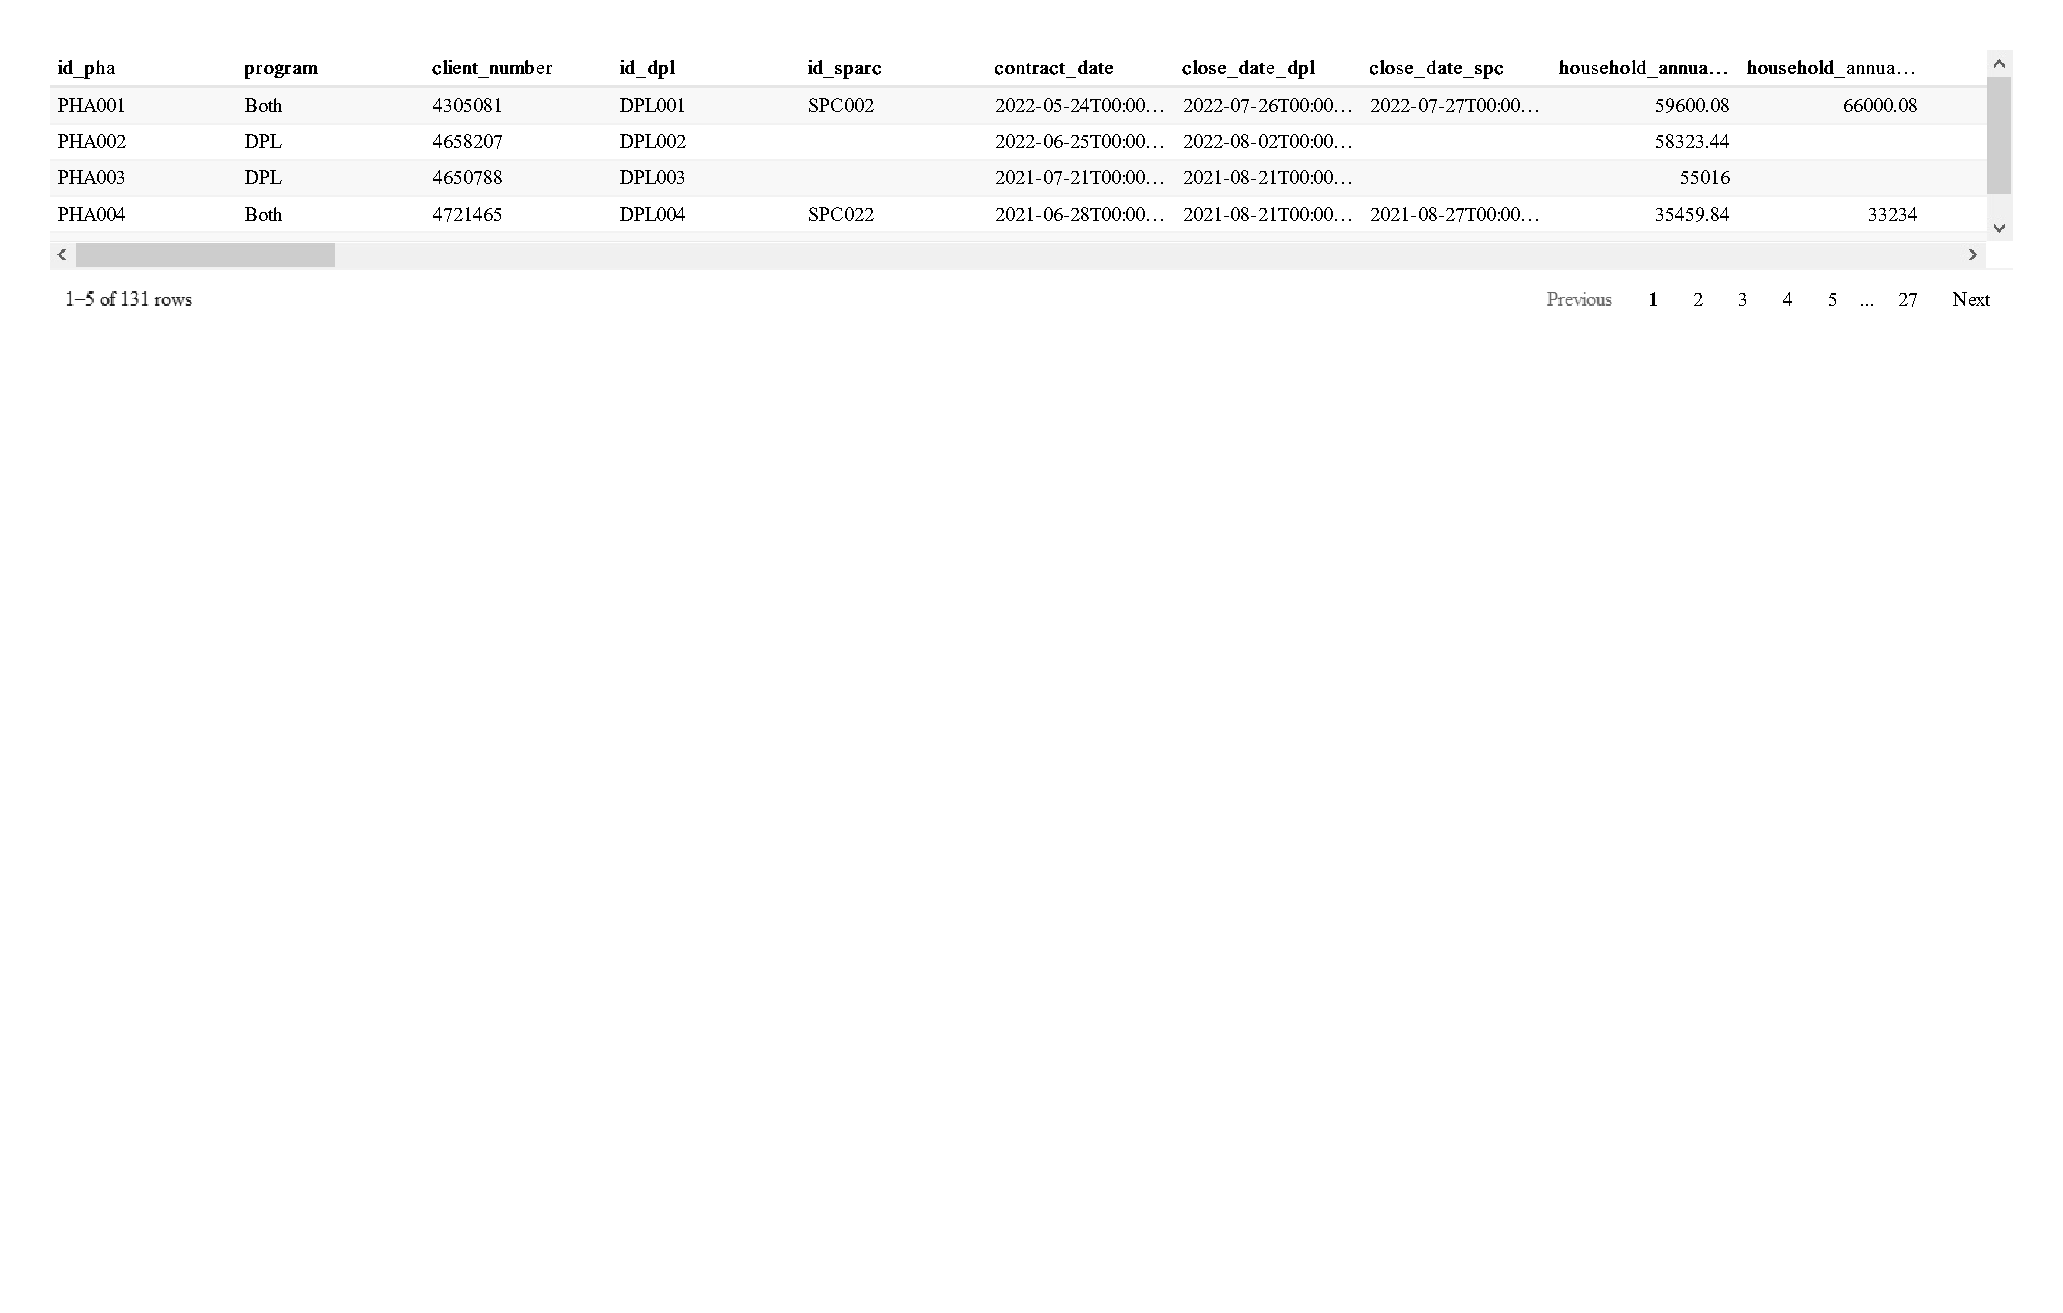
\includegraphics{piedmont_files/figure-pdf/dpl-table-1.pdf}

}

\end{figure}

Where there were duplicate fields from each dataset, the \texttt{\_dpl}
and \texttt{\_spc} suffixes were added to the end of column names,
respective to their source. For example, the close date data from the
DPL records are retained as the \texttt{close\_date\_dpl} column, while
the close dates from the SPARC data are \texttt{close\_date\_spc}.

\begin{tcolorbox}[enhanced jigsaw, coltitle=black, titlerule=0mm, breakable, colbacktitle=quarto-callout-warning-color!10!white, opacityback=0, leftrule=.75mm, opacitybacktitle=0.6, rightrule=.15mm, title=\textcolor{quarto-callout-warning-color}{\faExclamationTriangle}\hspace{0.5em}{Data integrity issues}, arc=.35mm, colback=white, bottomtitle=1mm, toptitle=1mm, colframe=quarto-callout-warning-color-frame, bottomrule=.15mm, toprule=.15mm, left=2mm]

Both the DPL and SPARC datasets were found to have data integrity issues
that PHA should resolve in the future.

\begin{itemize}
\item
  Mortgage product fields included both ``RHS'' (Rural Housing Service),
  ``USDA'', and ``502'' values. For now, these are all assumed to be
  ``502 Direct Loans''.
\item
  Overlapping fields from the DPL and SPARC datasets do not always
  reconcile for the clients who used both programs. For example, the
  specific close dates and household income values are often slightly
  different---but should, in theory, be identical.
\item
  The SPARC client records are missing many values in the closing date,
  interest rate, household income, household size, and lender columns.
\item
  Some DPL clients were noted as receiving SPARC in the
  \texttt{other\_assistance} column. However, two of clients were
  \emph{not} found in the SPARC data.
\end{itemize}

\end{tcolorbox}

\hypertarget{regional-and-neighborhood-profiles}{%
\subsection{Regional and neighborhood
profiles}\label{regional-and-neighborhood-profiles}}

\begin{tcolorbox}[enhanced jigsaw, coltitle=black, titlerule=0mm, breakable, colbacktitle=quarto-callout-tip-color!10!white, opacityback=0, leftrule=.75mm, opacitybacktitle=0.6, rightrule=.15mm, title=\textcolor{quarto-callout-tip-color}{\faLightbulb}\hspace{0.5em}{Why this is needed}, arc=.35mm, colback=white, bottomtitle=1mm, toptitle=1mm, colframe=quarto-callout-tip-color-frame, bottomrule=.15mm, toprule=.15mm, left=2mm]

Demographic and socioeconomic data will help establish the baseline
characteristics of population groups that PHA seeks to compare with its
clients. For example, how closely does the client pool match the average
racial and ethnic makeup across the region?

\end{tcolorbox}

Two datasets will be used to create summary profiles of the geographies
PHA will use as reference for its clients' characteristics. Both are
from the U.S. Census Bureau:

\begin{itemize}
\tightlist
\item
  2020 Decennial Census
\item
  American Community Survey (5-year estimates)
\end{itemize}

\begin{tcolorbox}[enhanced jigsaw, coltitle=black, titlerule=0mm, breakable, colbacktitle=quarto-callout-note-color!10!white, opacityback=0, leftrule=.75mm, opacitybacktitle=0.6, rightrule=.15mm, title=\textcolor{quarto-callout-note-color}{\faInfo}\hspace{0.5em}{Note}, arc=.35mm, colback=white, bottomtitle=1mm, toptitle=1mm, colframe=quarto-callout-note-color-frame, bottomrule=.15mm, toprule=.15mm, left=2mm]

As of June 2023, the latest ACS data available are the 2017-2021 5-year
estimates.

\end{tcolorbox}

The fields to collect from this data include:

\begin{itemize}
\tightlist
\item
  Race and ethnicity of population
\item
  Average household incomes
\item
  Homeownership rates
\end{itemize}

\textbf{Step 1: Race and ethnicity data from 2020 Census}

\begin{Shaded}
\begin{Highlighting}[]
\CommentTok{\# Get variables for 2020 Census PL{-}94171 Redistricting dataset}

\NormalTok{pl\_vars }\OtherTok{\textless{}{-}} \FunctionTok{load\_variables}\NormalTok{(}\DecValTok{2020}\NormalTok{, }\StringTok{"pl"}\NormalTok{, }\AttributeTok{cache =} \ConstantTok{TRUE}\NormalTok{)}

\CommentTok{\# Find and select race and ethnicity variables}

\NormalTok{race\_vars }\OtherTok{\textless{}{-}}\NormalTok{ pl\_vars }\SpecialCharTok{|\textgreater{}} 
  \FunctionTok{filter}\NormalTok{(name }\SpecialCharTok{\%in\%} \FunctionTok{c}\NormalTok{(}
    \StringTok{"P1\_003N"}\NormalTok{, }\CommentTok{\# White}
    \StringTok{"P1\_004N"}\NormalTok{, }\CommentTok{\# Black}
    \StringTok{"P1\_005N"}\NormalTok{, }\CommentTok{\# American Indian and Alaska Native}
    \StringTok{"P1\_006N"}\NormalTok{, }\CommentTok{\# Asian}
    \StringTok{"P1\_007N"}\NormalTok{, }\CommentTok{\# Native Hawaiian and Other Pacific Islander}
    \StringTok{"P1\_008N"}\NormalTok{, }\CommentTok{\# Some other race}
    \StringTok{"P1\_009N"}\NormalTok{, }\CommentTok{\# Two or more races}
    \StringTok{"P2\_002N"}\NormalTok{, }\CommentTok{\# Total Hispanic or Latino}
    \StringTok{"P2\_003N"}  \CommentTok{\# Total not Hispanic or Latino}
\NormalTok{  )) }\SpecialCharTok{|\textgreater{}} 
  
  \CommentTok{\# Rename race and ethnicity groups }
  
  \FunctionTok{mutate}\NormalTok{(}\AttributeTok{label =} \FunctionTok{case\_when}\NormalTok{(}
\NormalTok{    name }\SpecialCharTok{==} \StringTok{"P1\_003N"} \SpecialCharTok{\textasciitilde{}} \StringTok{"White"}\NormalTok{,}
\NormalTok{    name }\SpecialCharTok{==} \StringTok{"P1\_004N"} \SpecialCharTok{\textasciitilde{}} \StringTok{"Black"}\NormalTok{,}
\NormalTok{    name }\SpecialCharTok{==} \StringTok{"P1\_005N"} \SpecialCharTok{\textasciitilde{}} \StringTok{"Another race"}\NormalTok{,}
\NormalTok{    name }\SpecialCharTok{==} \StringTok{"P1\_006N"} \SpecialCharTok{\textasciitilde{}} \StringTok{"Asian"}\NormalTok{,}
\NormalTok{    name }\SpecialCharTok{==} \StringTok{"P1\_007N"} \SpecialCharTok{\textasciitilde{}} \StringTok{"Another race"}\NormalTok{,}
\NormalTok{    name }\SpecialCharTok{==} \StringTok{"P1\_008N"} \SpecialCharTok{\textasciitilde{}} \StringTok{"Another race"}\NormalTok{,}
\NormalTok{    name }\SpecialCharTok{==} \StringTok{"P1\_009N"} \SpecialCharTok{\textasciitilde{}} \StringTok{"Multiracial"}\NormalTok{,}
\NormalTok{    name }\SpecialCharTok{==} \StringTok{"P2\_002N"} \SpecialCharTok{\textasciitilde{}} \StringTok{"Hispanic or Latino"}\NormalTok{,}
\NormalTok{    name }\SpecialCharTok{==} \StringTok{"P2\_003N"} \SpecialCharTok{\textasciitilde{}} \StringTok{"Not Hispanic or Latino"}\NormalTok{,}
\NormalTok{  )) }\SpecialCharTok{|\textgreater{}} 
  
  \CommentTok{\# Add race/ethnicity label}
  
  \FunctionTok{mutate}\NormalTok{(}\AttributeTok{category =} \FunctionTok{case\_when}\NormalTok{(}
      \FunctionTok{str\_detect}\NormalTok{(name, }\StringTok{"P1"}\NormalTok{) }\SpecialCharTok{\textasciitilde{}} \StringTok{"Race"}\NormalTok{,}
      \ConstantTok{TRUE} \SpecialCharTok{\textasciitilde{}} \StringTok{"Ethnicity"}\NormalTok{),}
    \AttributeTok{.after =} \DecValTok{1}
\NormalTok{  ) }\SpecialCharTok{|\textgreater{}} 
  
  \CommentTok{\# Drop concept column (unneeded)}
  
  \FunctionTok{select}\NormalTok{(}\SpecialCharTok{{-}}\NormalTok{concept)}

\CommentTok{\# Import 2020 Census race and ethnicity data for Charlottesville City}

\NormalTok{cv\_race\_raw }\OtherTok{\textless{}{-}} \FunctionTok{get\_decennial}\NormalTok{(}
  \AttributeTok{geography =} \StringTok{"county"}\NormalTok{,}
  \AttributeTok{variables =}\NormalTok{ race\_vars}\SpecialCharTok{$}\NormalTok{name,}
  \AttributeTok{year =} \DecValTok{2020}\NormalTok{,}
  \AttributeTok{sumfile =} \StringTok{"pl"}\NormalTok{,}
  \AttributeTok{state =} \StringTok{"VA"}\NormalTok{,}
  \AttributeTok{county =} \StringTok{"Charlottesville city"}\NormalTok{,}
  \AttributeTok{cache\_table =} \ConstantTok{TRUE}
\NormalTok{)}
\end{Highlighting}
\end{Shaded}

\begin{Shaded}
\begin{Highlighting}[]
\CommentTok{\# Join race and ethnicity labels}

\NormalTok{cv\_race }\OtherTok{\textless{}{-}}\NormalTok{ cv\_race\_raw }\SpecialCharTok{|\textgreater{}} 
  \FunctionTok{left\_join}\NormalTok{(race\_vars, }\AttributeTok{by =} \FunctionTok{c}\NormalTok{(}\StringTok{"variable"} \OtherTok{=} \StringTok{"name"}\NormalTok{)) }\SpecialCharTok{|\textgreater{}} 
  
  \CommentTok{\# Sum "Another race" values into one row}
  
  \FunctionTok{group\_by}\NormalTok{(category, label) }\SpecialCharTok{|\textgreater{}} 
  \FunctionTok{summarise}\NormalTok{(}\AttributeTok{value =} \FunctionTok{sum}\NormalTok{(value)) }\SpecialCharTok{|\textgreater{}} 
  
  \CommentTok{\# Add percent column}
  
  \FunctionTok{group\_by}\NormalTok{(category) }\SpecialCharTok{|\textgreater{}} 
  \FunctionTok{mutate}\NormalTok{(}\AttributeTok{pct =}\NormalTok{ value}\SpecialCharTok{/}\FunctionTok{sum}\NormalTok{(value)) }\SpecialCharTok{|\textgreater{}} 
  \FunctionTok{ungroup}\NormalTok{()}

\CommentTok{\# Generate table}

\NormalTok{cv\_race }\SpecialCharTok{|\textgreater{}} 
  \FunctionTok{arrange}\NormalTok{(}\FunctionTok{desc}\NormalTok{(value), }\AttributeTok{.by\_group =} \ConstantTok{TRUE}\NormalTok{) }\SpecialCharTok{|\textgreater{}} 
  \FunctionTok{kable}\NormalTok{() }\SpecialCharTok{|\textgreater{}} 
\NormalTok{  kableExtra}\SpecialCharTok{::}\FunctionTok{kable\_styling}\NormalTok{(}
    \AttributeTok{bootstrap\_options =} \FunctionTok{c}\NormalTok{(}\StringTok{"striped"}\NormalTok{, }\StringTok{"hover"}\NormalTok{, }\StringTok{"condensed"}\NormalTok{, }\StringTok{"responsive"}\NormalTok{)}
\NormalTok{  )}
\end{Highlighting}
\end{Shaded}

\begin{table}
\centering
\begin{tabular}{l|l|r|r}
\hline
category & label & value & pct\\
\hline
Ethnicity & Not Hispanic or Latino & 43346 & 0.9311108\\
\hline
Race & White & 30344 & 0.6518162\\
\hline
Race & Black & 7122 & 0.1529869\\
\hline
Race & Asian & 4083 & 0.0877065\\
\hline
Race & Multiracial & 3583 & 0.0769660\\
\hline
Ethnicity & Hispanic or Latino & 3207 & 0.0688892\\
\hline
Race & Another race & 1421 & 0.0305243\\
\hline
\end{tabular}
\end{table}

\textbf{Step 2: Household income data from ACS}

\begin{Shaded}
\begin{Highlighting}[]
\CommentTok{\# Get variables for Table B25118: Tenure by Household Income}

\NormalTok{b25118\_vars }\OtherTok{\textless{}{-}} \FunctionTok{load\_variables}\NormalTok{(}\DecValTok{2021}\NormalTok{, }\StringTok{"acs5"}\NormalTok{, }\AttributeTok{cache =} \ConstantTok{TRUE}\NormalTok{) }\SpecialCharTok{|\textgreater{}} 
  \FunctionTok{filter}\NormalTok{(}\FunctionTok{str\_sub}\NormalTok{(name, }\AttributeTok{end =} \DecValTok{6}\NormalTok{) }\SpecialCharTok{\%in\%} \StringTok{"B25118"}\NormalTok{)}

\CommentTok{\# Clean variables}

\NormalTok{inc\_vars }\OtherTok{\textless{}{-}}\NormalTok{ b25118\_vars }\SpecialCharTok{|\textgreater{}} 
  \FunctionTok{separate}\NormalTok{(label, }\FunctionTok{c}\NormalTok{(}\StringTok{"est"}\NormalTok{, }\StringTok{"total"}\NormalTok{, }\StringTok{"tenure"}\NormalTok{, }\StringTok{"income"}\NormalTok{), }\AttributeTok{sep =} \StringTok{"!!"}\NormalTok{) }\SpecialCharTok{|\textgreater{}} 
  \FunctionTok{select}\NormalTok{(}\DecValTok{1}\NormalTok{, }\DecValTok{4}\NormalTok{, }\DecValTok{5}\NormalTok{) }\SpecialCharTok{|\textgreater{}} 
  \FunctionTok{drop\_na}\NormalTok{() }\SpecialCharTok{|\textgreater{}} 
  \FunctionTok{mutate}\NormalTok{(}\AttributeTok{tenure =} \FunctionTok{str\_remove\_all}\NormalTok{(tenure, }\StringTok{" occupied:"}\NormalTok{),}
         \AttributeTok{tenure =} \FunctionTok{str\_replace\_all}\NormalTok{(tenure, }\StringTok{"Owner"}\NormalTok{, }\StringTok{"Homeowner"}\NormalTok{))}

\CommentTok{\# Import 2021 ACS estimates}

\NormalTok{b25118\_raw }\OtherTok{\textless{}{-}} \FunctionTok{get\_acs}\NormalTok{(}
  \AttributeTok{geography =} \StringTok{"county"}\NormalTok{,}
  \AttributeTok{variables =}\NormalTok{ inc\_vars}\SpecialCharTok{$}\NormalTok{name,}
  \AttributeTok{year =} \DecValTok{2021}\NormalTok{,}
  \AttributeTok{county =} \StringTok{"Charlottesville city"}\NormalTok{,}
  \AttributeTok{state =} \StringTok{"VA"}\NormalTok{,}
  \AttributeTok{cache\_table =} \ConstantTok{TRUE}
\NormalTok{)}
\end{Highlighting}
\end{Shaded}

\begin{Shaded}
\begin{Highlighting}[]
\CommentTok{\# Join variables to data}

\NormalTok{cv\_income }\OtherTok{\textless{}{-}}\NormalTok{ b25118\_raw }\SpecialCharTok{|\textgreater{}} 
  \FunctionTok{left\_join}\NormalTok{(inc\_vars, }\AttributeTok{by =} \FunctionTok{c}\NormalTok{(}\StringTok{"variable"} \OtherTok{=} \StringTok{"name"}\NormalTok{)) }\SpecialCharTok{|\textgreater{}} 
  
  \CommentTok{\# Remove unnecessary columns and rearrange}
  
  \FunctionTok{select}\NormalTok{(}\DecValTok{6}\NormalTok{, }\DecValTok{7}\NormalTok{, }\DecValTok{4}\NormalTok{) }\SpecialCharTok{|\textgreater{}} 
  
  \CommentTok{\# Collapse into fewer income categories}
  
  \FunctionTok{mutate}\NormalTok{(}\AttributeTok{income =} \FunctionTok{case\_when}\NormalTok{(}
\NormalTok{    income }\SpecialCharTok{==} \StringTok{"Less than $5,000"} \SpecialCharTok{\textasciitilde{}} \StringTok{"Less than $35,000"}\NormalTok{,}
\NormalTok{    income }\SpecialCharTok{==} \StringTok{"$5,000 to $9,999"} \SpecialCharTok{\textasciitilde{}} \StringTok{"Less than $35,000"}\NormalTok{,}
\NormalTok{    income }\SpecialCharTok{==} \StringTok{"$10,000 to $14,999"} \SpecialCharTok{\textasciitilde{}} \StringTok{"Less than $35,000"}\NormalTok{,}
\NormalTok{    income }\SpecialCharTok{==} \StringTok{"$15,000 to $19,999"} \SpecialCharTok{\textasciitilde{}} \StringTok{"Less than $35,000"}\NormalTok{,}
\NormalTok{    income }\SpecialCharTok{==} \StringTok{"$20,000 to $24,999"} \SpecialCharTok{\textasciitilde{}} \StringTok{"Less than $35,000"}\NormalTok{,}
\NormalTok{    income }\SpecialCharTok{==} \StringTok{"$25,000 to $34,999"} \SpecialCharTok{\textasciitilde{}} \StringTok{"Less than $35,000"}\NormalTok{,}
\NormalTok{    income }\SpecialCharTok{==} \StringTok{"$100,000 to $149,999"} \SpecialCharTok{\textasciitilde{}} \StringTok{"$100,000 or more"}\NormalTok{,}
\NormalTok{    income }\SpecialCharTok{==} \StringTok{"$150,000 or more"} \SpecialCharTok{\textasciitilde{}} \StringTok{"$100,000 or more"}\NormalTok{,}
    \ConstantTok{TRUE} \SpecialCharTok{\textasciitilde{}}\NormalTok{ income}
\NormalTok{  )) }\SpecialCharTok{|\textgreater{}} 
  \FunctionTok{group\_by}\NormalTok{(tenure, income) }\SpecialCharTok{|\textgreater{}} 
  \FunctionTok{summarise}\NormalTok{(}\AttributeTok{estimate =} \FunctionTok{sum}\NormalTok{(estimate))}

\CommentTok{\# Generate table}

\NormalTok{cv\_income }\SpecialCharTok{|\textgreater{}} 
  \FunctionTok{ungroup}\NormalTok{() }\SpecialCharTok{|\textgreater{}} 
  \FunctionTok{mutate}\NormalTok{(}\AttributeTok{income =} \FunctionTok{fct\_relevel}\NormalTok{(income, }\StringTok{"Less than $35,000"}\NormalTok{, }\StringTok{"$35,000 to $49,999"}\NormalTok{,}
                              \StringTok{"$50,000 to $74,999"}\NormalTok{, }\StringTok{"$75,000 to $99,999"}\NormalTok{,}
                              \StringTok{"$100,000 or more"}\NormalTok{)) }\SpecialCharTok{|\textgreater{}} 
  \FunctionTok{arrange}\NormalTok{(income) }\SpecialCharTok{|\textgreater{}} 
  \FunctionTok{kable}\NormalTok{() }\SpecialCharTok{|\textgreater{}} 
\NormalTok{  kableExtra}\SpecialCharTok{::}\FunctionTok{kable\_styling}\NormalTok{(}
    \AttributeTok{bootstrap\_options =} \FunctionTok{c}\NormalTok{(}\StringTok{"striped"}\NormalTok{, }\StringTok{"hover"}\NormalTok{, }\StringTok{"condensed"}\NormalTok{, }\StringTok{"responsive"}\NormalTok{)}
\NormalTok{  )}
\end{Highlighting}
\end{Shaded}

\begin{table}
\centering
\begin{tabular}{l|l|r}
\hline
tenure & income & estimate\\
\hline
Homeowner & Less than \$35,000 & 883\\
\hline
Renter & Less than \$35,000 & 5140\\
\hline
Homeowner & \$35,000 to \$49,999 & 764\\
\hline
Renter & \$35,000 to \$49,999 & 1234\\
\hline
Homeowner & \$50,000 to \$74,999 & 861\\
\hline
Renter & \$50,000 to \$74,999 & 1809\\
\hline
Homeowner & \$75,000 to \$99,999 & 1171\\
\hline
Renter & \$75,000 to \$99,999 & 985\\
\hline
Homeowner & \$100,000 or more & 4300\\
\hline
Renter & \$100,000 or more & 2165\\
\hline
\end{tabular}
\end{table}

\textbf{Step 3: Homeownership data from ACS}

\begin{Shaded}
\begin{Highlighting}[]
\CommentTok{\# tbd}
\end{Highlighting}
\end{Shaded}

\begin{Shaded}
\begin{Highlighting}[]
\CommentTok{\# tbd}
\end{Highlighting}
\end{Shaded}

\hypertarget{mortgage-applications-and-activity}{%
\subsection{Mortgage applications and
activity}\label{mortgage-applications-and-activity}}

\begin{tcolorbox}[enhanced jigsaw, coltitle=black, titlerule=0mm, breakable, colbacktitle=quarto-callout-tip-color!10!white, opacityback=0, leftrule=.75mm, opacitybacktitle=0.6, rightrule=.15mm, title=\textcolor{quarto-callout-tip-color}{\faLightbulb}\hspace{0.5em}{Why this is needed}, arc=.35mm, colback=white, bottomtitle=1mm, toptitle=1mm, colframe=quarto-callout-tip-color-frame, bottomrule=.15mm, toprule=.15mm, left=2mm]

Along with comparing client characteristics with the region or a
neighborhood as a whole, we can compare their mortgages to overall
lending activity in the community over time. This will allow PHA to
benchmark its buyer assistance efforts to home loan trends across the
region.

\end{tcolorbox}

This information is available from the Home Mortgage Disclosure Act
(HMDA) data from the Consumer Financial Protection Bureau. HMDA data
include loan-level information on buyer demographics, loan attributes,
and property characteristics. Entries for buyers whose applications were
eventually withdrawn or denied are also included.

\begin{tcolorbox}[enhanced jigsaw, coltitle=black, titlerule=0mm, breakable, colbacktitle=quarto-callout-note-color!10!white, opacityback=0, leftrule=.75mm, opacitybacktitle=0.6, rightrule=.15mm, title=\textcolor{quarto-callout-note-color}{\faInfo}\hspace{0.5em}{Note}, arc=.35mm, colback=white, bottomtitle=1mm, toptitle=1mm, colframe=quarto-callout-note-color-frame, bottomrule=.15mm, toprule=.15mm, left=2mm]

As of June 2023, the latest HMDA data available is for 2021.

\end{tcolorbox}

The fields to collect from this data include:

\begin{itemize}
\tightlist
\item
  Buyer race and ethnicity
\item
  Buyer county and census tract
\item
  Loan type (conventional, FHA, VA, or USDA)
\item
  Action taken (loan originated, application denied or withdrawn)
\item
  Loan amount
\item
  Interest rate
\item
  Property value
\item
  Occupancy type (principal residence only)
\item
  Buyer gross annual income
\item
  Debt-to-income ratio
\end{itemize}

\begin{tcolorbox}[enhanced jigsaw, coltitle=black, titlerule=0mm, breakable, colbacktitle=quarto-callout-caution-color!10!white, opacityback=0, leftrule=.75mm, opacitybacktitle=0.6, rightrule=.15mm, title=\textcolor{quarto-callout-caution-color}{\faFire}\hspace{0.5em}{Future work}, arc=.35mm, colback=white, bottomtitle=1mm, toptitle=1mm, colframe=quarto-callout-caution-color-frame, bottomrule=.15mm, toprule=.15mm, left=2mm]

This data was not collected within the scope of the original project.
Analysis with this data could be completed as a future update.

\end{tcolorbox}

\hypertarget{home-values}{%
\subsection{Home values}\label{home-values}}

\begin{tcolorbox}[enhanced jigsaw, coltitle=black, titlerule=0mm, breakable, colbacktitle=quarto-callout-tip-color!10!white, opacityback=0, leftrule=.75mm, opacitybacktitle=0.6, rightrule=.15mm, title=\textcolor{quarto-callout-tip-color}{\faLightbulb}\hspace{0.5em}{Why this is needed}, arc=.35mm, colback=white, bottomtitle=1mm, toptitle=1mm, colframe=quarto-callout-tip-color-frame, bottomrule=.15mm, toprule=.15mm, left=2mm]

Detailed data on home sales and values are necessary to make estimates
about the total home equity gained (or lost) by PHA buyers and other
homeowners in the community. This property-level data will help PHA
assess its programs' abilities to support wealth-building among clients.

\end{tcolorbox}

\hypertarget{real-estate-assessments}{%
\subsubsection{Real estate assessments}\label{real-estate-assessments}}

Localities in PHA's service area regularly assess property values to
calculate the total real estate taxes to be paid by each property owner.
Properties are reassessed to better match taxable values with potential
market values, which can change significantly over time.

Despite these updates, local assessments can often lag behind current
market trends, so they are not the most accurate indicator of the actual
market value of a home if it were sold. Still, assessment data are
consistent and publicly available for all parcels in a locality. This
creates a useful longitudinal dataset.

For this preliminary analysis, only assessment data from the City of
Charlottesville will be used.

The fields to collect from this data include:

\begin{itemize}
\tightlist
\item
  Parcel number
\item
  Street number and name
\item
  Bedrooms and bathrooms
\item
  Finished square footage
\item
  Total assessed value
\end{itemize}

\begin{Shaded}
\begin{Highlighting}[]
\CommentTok{\# Load in multi{-}year assessment data}

\NormalTok{cv\_assess }\OtherTok{\textless{}{-}} \FunctionTok{read\_csv}\NormalTok{(}\StringTok{"data/raw/Real\_Estate\_(All\_Assessments).csv"}\NormalTok{) }\SpecialCharTok{|\textgreater{}} 
  
  \CommentTok{\# Filter tax years 2017 and later}
  
  \FunctionTok{filter}\NormalTok{(TaxYear }\SpecialCharTok{\textgreater{}} \DecValTok{2016}\NormalTok{) }\SpecialCharTok{|\textgreater{}} 
  
  \CommentTok{\# Keep only relevant fields}
  
  \FunctionTok{select}\NormalTok{(ParcelNumber, TotalValue, TaxYear)}
\end{Highlighting}
\end{Shaded}

\begin{Shaded}
\begin{Highlighting}[]
\CommentTok{\# Load in detailed residential property data}

\NormalTok{cv\_residential }\OtherTok{\textless{}{-}} \FunctionTok{read\_csv}\NormalTok{(}\StringTok{"data/raw/Real\_Estate\_(Residential\_Details).csv"}\NormalTok{) }\SpecialCharTok{|\textgreater{}} 
  
  \CommentTok{\# Filter for single{-}family types only}
  
  \FunctionTok{filter}\NormalTok{(}\FunctionTok{str\_detect}\NormalTok{(UseCode, }\StringTok{"Single Family"}\NormalTok{)) }\SpecialCharTok{|\textgreater{}} 
  
  \CommentTok{\# Keep only relevant fields}
  
  \FunctionTok{select}\NormalTok{(ParcelNumber, StreetNumber, StreetName, Bedrooms, HalfBathrooms,}
\NormalTok{         FullBathrooms, }\AttributeTok{SqFt =}\NormalTok{ SquareFootageFinishedLiving)}

\CommentTok{\# Load shapefile of parcels}

\NormalTok{cv\_parcels }\OtherTok{\textless{}{-}} \FunctionTok{st\_read}\NormalTok{(}\StringTok{"data/shp/Parcel\_Area\_Details.shp"}\NormalTok{) }\SpecialCharTok{|\textgreater{}} 
  
  \CommentTok{\# Project into Virginia State Plane South}
  
  \FunctionTok{st\_transform}\NormalTok{(}\DecValTok{4502}\NormalTok{) }\SpecialCharTok{|\textgreater{}} 
  
  \CommentTok{\# Fix column name}
  
  \FunctionTok{select}\NormalTok{(}\AttributeTok{ParcelNumber =}\NormalTok{ ParcelNumb) }\SpecialCharTok{|\textgreater{}} 
  
  \CommentTok{\# Join to detailed residential property data}
  
  \FunctionTok{right\_join}\NormalTok{(cv\_residential, }\AttributeTok{by =} \StringTok{"ParcelNumber"}\NormalTok{)}

\CommentTok{\# Save data}

\FunctionTok{write\_rds}\NormalTok{(cv\_parcels, }\StringTok{"data/cv\_parcels.rds"}\NormalTok{)}
\end{Highlighting}
\end{Shaded}

\hypertarget{mls-sales}{%
\subsubsection{MLS sales}\label{mls-sales}}

Actual recorded home sales are the most accurate way to determine
residential property values. For arms-length transactions, sales prices
reflect the actual market value of each home. These records are
therefore the ideal source to best determine home equity changes among
homeowners.

PHA is able to provide data exported from the multiple listing service
(MLS) operated by the Charlottesville Area Association of REALTORS®
(CAAR). The MLS platform includes all real estate listings from agents
in the region and is dynamically updated as listings are added, updated,
or closed.

For this preliminary analysis, PHA has provided data on all sold
single-family homes in the City of Charlottesville from September 2022
through November 22, 2022.

Fields included in this exports include:

\begin{itemize}
\tightlist
\item
  Property address
\item
  Days on market
\item
  List price
\item
  Closed date
\item
  Bedrooms and bathrooms
\item
  Finished square footage
\end{itemize}

\begin{Shaded}
\begin{Highlighting}[]
\CommentTok{\# Load in records exported from MLS and clean column names}

\NormalTok{mls }\OtherTok{\textless{}{-}} \FunctionTok{read\_csv}\NormalTok{(}\StringTok{"data/raw/Default\_MLS\_Defined\_Spreadsheet.csv"}\NormalTok{) }\SpecialCharTok{|\textgreater{}} 
  \FunctionTok{clean\_names}\NormalTok{() }\SpecialCharTok{|\textgreater{}} 
  
  \CommentTok{\# Keep only relevant fields}
  
  \FunctionTok{select}\NormalTok{(address, city, closed\_date, number\_beds, number\_baths, total\_sq\_ft, list\_price)}
  
\CommentTok{\# Add state field and geocode addresses}

\NormalTok{mls\_geocode }\OtherTok{\textless{}{-}}\NormalTok{ mls }\SpecialCharTok{|\textgreater{}} 
  \FunctionTok{mutate}\NormalTok{(}\AttributeTok{state =} \StringTok{"VA"}\NormalTok{, }\AttributeTok{.before =} \DecValTok{3}\NormalTok{) }\SpecialCharTok{|\textgreater{}} 
  \FunctionTok{geocode}\NormalTok{(}\AttributeTok{street =}\NormalTok{ address,}
          \AttributeTok{state =}\NormalTok{ state,}
          \AttributeTok{city =}\NormalTok{ city,}
          \AttributeTok{method =} \StringTok{"geocodio"}\NormalTok{,}
          \AttributeTok{lat =}\NormalTok{ lat,}
          \AttributeTok{long =}\NormalTok{ long) }\SpecialCharTok{|\textgreater{}} 
  
  \CommentTok{\# Drop records that did not match}
  
  \FunctionTok{drop\_na}\NormalTok{(lat) }\SpecialCharTok{|\textgreater{}} 
  
  \CommentTok{\# Specify WGS 1984 coordinate system for lat/long data}
  
  \FunctionTok{st\_as\_sf}\NormalTok{(}\AttributeTok{coords =} \FunctionTok{c}\NormalTok{(}\StringTok{"long"}\NormalTok{, }\StringTok{"lat"}\NormalTok{),}
           \AttributeTok{remove =} \ConstantTok{FALSE}\NormalTok{,}
           \AttributeTok{crs =} \DecValTok{4326}\NormalTok{) }\SpecialCharTok{|\textgreater{}} 
  
  \CommentTok{\# Project into Virginia State Plane South}
  
  \FunctionTok{st\_transform}\NormalTok{(}\DecValTok{4502}\NormalTok{)}

\CommentTok{\# Save data}

\FunctionTok{write\_rds}\NormalTok{(mls\_geocode, }\StringTok{"data/mls\_geocode.rds"}\NormalTok{)}
\end{Highlighting}
\end{Shaded}

\hypertarget{public-sales-records}{%
\subsubsection{Public sales records}\label{public-sales-records}}

The City of Charlottesville also maintains a
\href{https://opendata.charlottesville.org/maps/real-estate-sales}{public
record of real estate transactions} on their open data portal. This data
is accessed and used in the Section~\ref{sec-home-equity} section.

\hypertarget{analysis}{%
\section{Analysis}\label{analysis}}

\hypertarget{clients-served-by-program}{%
\subsection{Clients served by program}\label{clients-served-by-program}}

From July 2017 through September 2022, PHA served a total of 131
households with its DPL and SPARC programs.

\begin{Shaded}
\begin{Highlighting}[]
\CommentTok{\# Cumulative total served by program}

\NormalTok{clients\_total }\OtherTok{\textless{}{-}}\NormalTok{ clients\_all }\SpecialCharTok{|\textgreater{}} 
  \FunctionTok{select}\NormalTok{(program, close\_date\_dpl, close\_date\_spc) }\SpecialCharTok{|\textgreater{}} 
  
  \CommentTok{\# Collapse close dates into one column}
  \CommentTok{\# Assume DPL close date is correct when SPARC date differs}
  
  \FunctionTok{mutate}\NormalTok{(}\AttributeTok{close\_date =} \FunctionTok{case\_when}\NormalTok{(}
    \SpecialCharTok{!}\FunctionTok{is.na}\NormalTok{(close\_date\_dpl) }\SpecialCharTok{\textasciitilde{}}\NormalTok{ close\_date\_dpl,}
    \ConstantTok{TRUE} \SpecialCharTok{\textasciitilde{}}\NormalTok{ close\_date\_spc}
\NormalTok{  ))}
  
\CommentTok{\# Summarise clients by month}

\NormalTok{clients\_cum }\OtherTok{\textless{}{-}}\NormalTok{ clients\_total }\SpecialCharTok{|\textgreater{}} 
  \FunctionTok{drop\_na}\NormalTok{(close\_date) }\SpecialCharTok{|\textgreater{}}     
  \FunctionTok{count}\NormalTok{(program, }\AttributeTok{month =} \FunctionTok{floor\_date}\NormalTok{(close\_date, }\StringTok{"month"}\NormalTok{)) }\SpecialCharTok{|\textgreater{}} 
  \FunctionTok{ungroup}\NormalTok{() }\SpecialCharTok{|\textgreater{}} 
  \FunctionTok{complete}\NormalTok{(program, month, }\AttributeTok{fill =} \FunctionTok{list}\NormalTok{(}\AttributeTok{n =} \DecValTok{0}\NormalTok{)) }\SpecialCharTok{|\textgreater{}} 
  
  \CommentTok{\# Cumulative sum by program}
  
  \FunctionTok{group\_by}\NormalTok{(program) }\SpecialCharTok{|\textgreater{}}
  \FunctionTok{mutate}\NormalTok{(}\AttributeTok{cum\_sum =} \FunctionTok{cumsum}\NormalTok{(n))}
  
\CommentTok{\# Create plot}

\FunctionTok{ggplot}\NormalTok{(clients\_cum, }\FunctionTok{aes}\NormalTok{(}\AttributeTok{x =}\NormalTok{ month, }\AttributeTok{y =}\NormalTok{ cum\_sum, }\AttributeTok{fill =}\NormalTok{ program)) }\SpecialCharTok{+}
  \FunctionTok{geom\_area}\NormalTok{() }\SpecialCharTok{+}
  \FunctionTok{scale\_y\_continuous}\NormalTok{(}\AttributeTok{breaks =} \FunctionTok{c}\NormalTok{(}\DecValTok{25}\NormalTok{,}\DecValTok{50}\NormalTok{,}\DecValTok{75}\NormalTok{,}\DecValTok{100}\NormalTok{,}\DecValTok{125}\NormalTok{)) }\SpecialCharTok{+}
  \FunctionTok{scale\_fill\_hda}\NormalTok{() }\SpecialCharTok{+}
  \FunctionTok{labs}\NormalTok{(}\AttributeTok{title =} \StringTok{"Cumulative total of clients served by program"}\NormalTok{,}
       \AttributeTok{subtitle =} \StringTok{"Data from July 2017 through September 2022"}\NormalTok{,}
       \AttributeTok{caption =} \StringTok{"**Note:** Four records without close dates are omitted."}\NormalTok{) }\SpecialCharTok{+}
  \FunctionTok{theme\_hda}\NormalTok{() }\SpecialCharTok{+}
  \FunctionTok{add\_zero\_line}\NormalTok{(}\StringTok{"y"}\NormalTok{) }\SpecialCharTok{+}
  \FunctionTok{theme}\NormalTok{(}
    \AttributeTok{legend.position =} \StringTok{"top"}
\NormalTok{  )}
\end{Highlighting}
\end{Shaded}

\begin{figure}[H]

{\centering 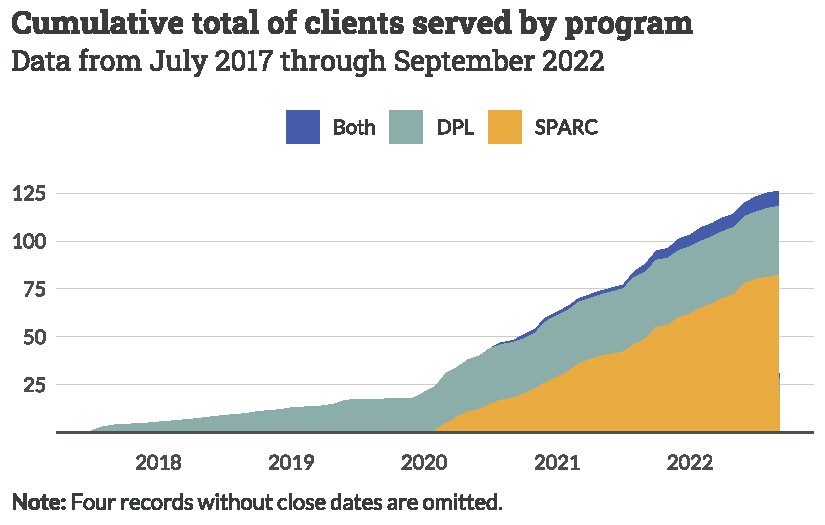
\includegraphics{piedmont_files/figure-pdf/cumulative-1.pdf}

}

\end{figure}

PHA served DPL-only clients from 2017 through 2019, averaging fewer than
ten annually. In 2020, PHA began offering SPARC, which has been used by
more than 25 clients annually since. Several clients have used both DPL
and SPARC assistance each year since 2020.

\begin{Shaded}
\begin{Highlighting}[]
\CommentTok{\# Summarise data by program and year}

\NormalTok{clients\_annual }\OtherTok{\textless{}{-}}\NormalTok{ clients\_total }\SpecialCharTok{|\textgreater{}} 
  \FunctionTok{drop\_na}\NormalTok{(close\_date) }\SpecialCharTok{|\textgreater{}}     
  \FunctionTok{count}\NormalTok{(program, }\AttributeTok{year =} \FunctionTok{floor\_date}\NormalTok{(close\_date, }\StringTok{"year"}\NormalTok{)) }\SpecialCharTok{|\textgreater{}} 
  \FunctionTok{ungroup}\NormalTok{() }\SpecialCharTok{|\textgreater{}} 
  \FunctionTok{complete}\NormalTok{(program, year, }\AttributeTok{fill =} \FunctionTok{list}\NormalTok{(}\AttributeTok{n =} \DecValTok{0}\NormalTok{)) }\SpecialCharTok{|\textgreater{}} 
  \FunctionTok{mutate}\NormalTok{(}\AttributeTok{year =} \FunctionTok{format}\NormalTok{(year, }\StringTok{"\%Y"}\NormalTok{))}

\CommentTok{\# Create plot}

\FunctionTok{ggplot}\NormalTok{(clients\_annual, }\FunctionTok{aes}\NormalTok{(}\AttributeTok{x =}\NormalTok{ year, }\AttributeTok{y =}\NormalTok{ n, }\AttributeTok{fill =}\NormalTok{ program)) }\SpecialCharTok{+}
  \FunctionTok{geom\_col}\NormalTok{(}\AttributeTok{position =} \StringTok{"stack"}\NormalTok{) }\SpecialCharTok{+}
  \FunctionTok{scale\_fill\_hda}\NormalTok{() }\SpecialCharTok{+}
  \FunctionTok{labs}\NormalTok{(}\AttributeTok{title =} \StringTok{"Annual number of clients served by program"}\NormalTok{,}
       \AttributeTok{subtitle =} \StringTok{"Data from July 2017 through September 2022"}\NormalTok{,}
       \AttributeTok{caption =} \StringTok{"**Note:** Four records without close dates are omitted."}\NormalTok{) }\SpecialCharTok{+}
  \FunctionTok{theme\_hda}\NormalTok{() }\SpecialCharTok{+}
  \FunctionTok{add\_zero\_line}\NormalTok{(}\StringTok{"y"}\NormalTok{) }\SpecialCharTok{+}
  \FunctionTok{theme}\NormalTok{(}
    \AttributeTok{legend.position =} \StringTok{"top"}
\NormalTok{  )}
\end{Highlighting}
\end{Shaded}

\begin{figure}[H]

{\centering 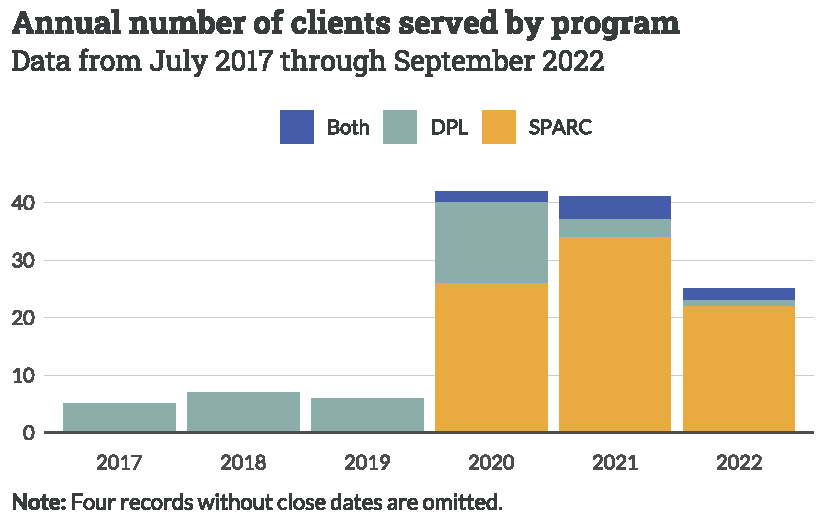
\includegraphics{piedmont_files/figure-pdf/annual-1.pdf}

}

\end{figure}

In total, two-thirds (66 percent) of all clients used SPARC only. About
one quarter (27 percent) used DPL only, and just eight clients (6
percent) took advantage of both.

\begin{Shaded}
\begin{Highlighting}[]
\CommentTok{\# Summarise data by program}

\NormalTok{clients\_program }\OtherTok{\textless{}{-}}\NormalTok{ clients\_total }\SpecialCharTok{|\textgreater{}}     
  \FunctionTok{count}\NormalTok{(program)}

\CommentTok{\# Create plot}

\FunctionTok{ggplot}\NormalTok{(clients\_program, }\FunctionTok{aes}\NormalTok{(}\AttributeTok{y =} \FunctionTok{reorder}\NormalTok{(program, n), }\AttributeTok{x =}\NormalTok{ n, }\AttributeTok{fill =}\NormalTok{ program, }\AttributeTok{label =}\NormalTok{ n)) }\SpecialCharTok{+}
  \FunctionTok{geom\_col}\NormalTok{() }\SpecialCharTok{+}
  \FunctionTok{geom\_text}\NormalTok{(}\AttributeTok{hjust =} \DecValTok{2}\NormalTok{,}
            \AttributeTok{color =} \StringTok{"white"}\NormalTok{,}
            \AttributeTok{size =} \DecValTok{5}\NormalTok{) }\SpecialCharTok{+}
  \FunctionTok{scale\_fill\_hda}\NormalTok{() }\SpecialCharTok{+}
  \FunctionTok{labs}\NormalTok{(}\AttributeTok{title =} \StringTok{"Total number of clients served by program"}\NormalTok{,}
       \AttributeTok{subtitle =} \StringTok{"Data from July 2017 through September 2022"}\NormalTok{) }\SpecialCharTok{+}
  \FunctionTok{theme\_hda}\NormalTok{() }\SpecialCharTok{+}
  \FunctionTok{add\_zero\_line}\NormalTok{(}\StringTok{"x"}\NormalTok{) }\SpecialCharTok{+}
  \FunctionTok{flip\_gridlines}\NormalTok{()}
\end{Highlighting}
\end{Shaded}

\begin{figure}[H]

{\centering 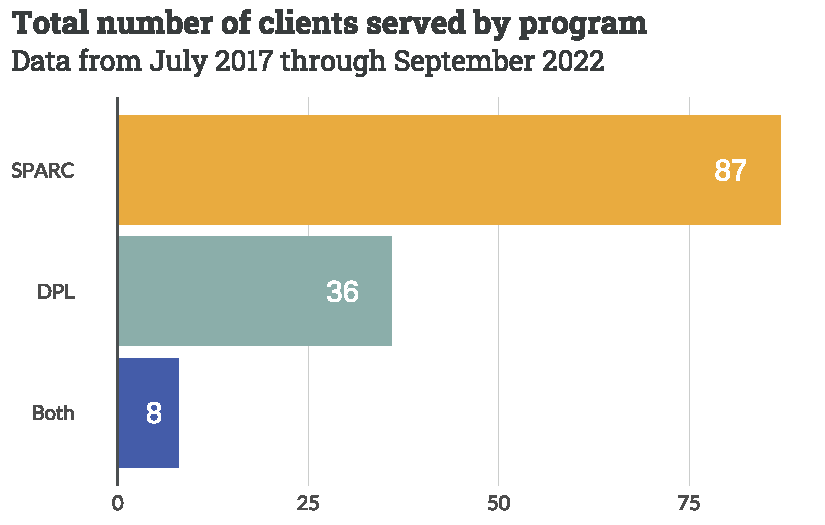
\includegraphics{piedmont_files/figure-pdf/totals-1.pdf}

}

\end{figure}

\hypertarget{profile-of-clients}{%
\subsection{Profile of clients}\label{profile-of-clients}}

\begin{tcolorbox}[enhanced jigsaw, coltitle=black, titlerule=0mm, breakable, colbacktitle=quarto-callout-warning-color!10!white, opacityback=0, leftrule=.75mm, opacitybacktitle=0.6, rightrule=.15mm, title=\textcolor{quarto-callout-warning-color}{\faExclamationTriangle}\hspace{0.5em}{Note}, arc=.35mm, colback=white, bottomtitle=1mm, toptitle=1mm, colframe=quarto-callout-warning-color-frame, bottomrule=.15mm, toprule=.15mm, left=2mm]

Race and ethnicity data is only available for clients who used the DPL
program.

\end{tcolorbox}

Among the 44 clients who used the DPL program, most were white (41
percent) or Black (34 percent). Another 11 percent were Asian, with the
remainder being multiracial or of another race. This is a more diverse
pattern than Charlottesville as a whole, where 65 percent of residents
are white, while only 15 percent of residents are Black, and 9 percent
are Asian.

The share of DPL clients who are Hispanic or Latino is about 7 percent,
which aligns very closely with the overall population of
Charlottesville.

\begin{Shaded}
\begin{Highlighting}[]
\CommentTok{\# Summarise clients by race}

\NormalTok{clients\_race }\OtherTok{\textless{}{-}}\NormalTok{ clients\_all }\SpecialCharTok{|\textgreater{}} 
  \FunctionTok{count}\NormalTok{(race) }\SpecialCharTok{|\textgreater{}} 
  \FunctionTok{drop\_na}\NormalTok{() }\SpecialCharTok{|\textgreater{}}
  \FunctionTok{ungroup}\NormalTok{() }\SpecialCharTok{|\textgreater{}} 
  
  \CommentTok{\# Add percent column}
  
  \FunctionTok{mutate}\NormalTok{(}\AttributeTok{pct =}\NormalTok{ n}\SpecialCharTok{/}\FunctionTok{sum}\NormalTok{(n)) }\SpecialCharTok{|\textgreater{}} 
  
  \CommentTok{\# Add source and category columns}
  
  \FunctionTok{mutate}\NormalTok{(}\AttributeTok{source =} \StringTok{"Clients"}\NormalTok{,}
         \AttributeTok{category =} \StringTok{"Race"}\NormalTok{,}
         \AttributeTok{.before =} \DecValTok{1}\NormalTok{) }\SpecialCharTok{|\textgreater{}} 
  
  \CommentTok{\# Update race labels and column names to match ACS data}
  
  \FunctionTok{mutate}\NormalTok{(}\AttributeTok{race =} \FunctionTok{case\_when}\NormalTok{(}
\NormalTok{    race }\SpecialCharTok{==} \StringTok{"Black and White"} \SpecialCharTok{\textasciitilde{}} \StringTok{"Multiracial"}\NormalTok{,}
\NormalTok{    race }\SpecialCharTok{==} \StringTok{"Other races"} \SpecialCharTok{\textasciitilde{}} \StringTok{"Another race"}\NormalTok{,}
    \ConstantTok{TRUE} \SpecialCharTok{\textasciitilde{}}\NormalTok{ race)) }\SpecialCharTok{|\textgreater{}} 
  \FunctionTok{rename}\NormalTok{(}\AttributeTok{label =}\NormalTok{ race,}
         \AttributeTok{value =}\NormalTok{ n)}

\CommentTok{\# Same as above for ethnicity}

\NormalTok{clients\_ethnicity }\OtherTok{\textless{}{-}}\NormalTok{ clients\_all }\SpecialCharTok{|\textgreater{}} 
  \FunctionTok{count}\NormalTok{(ethnicity) }\SpecialCharTok{|\textgreater{}} 
  \FunctionTok{drop\_na}\NormalTok{() }\SpecialCharTok{|\textgreater{}}
  \FunctionTok{ungroup}\NormalTok{() }\SpecialCharTok{|\textgreater{}} 
  
  \CommentTok{\# Add percent column}
  
  \FunctionTok{mutate}\NormalTok{(}\AttributeTok{pct =}\NormalTok{ n}\SpecialCharTok{/}\FunctionTok{sum}\NormalTok{(n)) }\SpecialCharTok{|\textgreater{}} 
  
  \CommentTok{\# Add source and category columns}
  
  \FunctionTok{mutate}\NormalTok{(}\AttributeTok{source =} \StringTok{"Clients"}\NormalTok{,}
         \AttributeTok{category =} \StringTok{"Ethnicity"}\NormalTok{,}
         \AttributeTok{.before =} \DecValTok{1}\NormalTok{) }\SpecialCharTok{|\textgreater{}} 
  
  \CommentTok{\# Update race labels and column names to match ACS data}
  
  \FunctionTok{mutate}\NormalTok{(}\AttributeTok{ethnicity =} \FunctionTok{case\_when}\NormalTok{(}
\NormalTok{    ethnicity }\SpecialCharTok{==} \StringTok{"Hispanic"} \SpecialCharTok{\textasciitilde{}} \StringTok{"Hispanic or Latino"}\NormalTok{,}
\NormalTok{    ethnicity }\SpecialCharTok{==} \StringTok{"Not Hispanic"} \SpecialCharTok{\textasciitilde{}} \StringTok{"Not Hispanic or Latino"}\NormalTok{,}
    \ConstantTok{TRUE} \SpecialCharTok{\textasciitilde{}}\NormalTok{ ethnicity)) }\SpecialCharTok{|\textgreater{}} 
  \FunctionTok{rename}\NormalTok{(}\AttributeTok{label =}\NormalTok{ ethnicity,}
         \AttributeTok{value =}\NormalTok{ n)}

\CommentTok{\# Add client data to ACS data}

\NormalTok{race\_join }\OtherTok{\textless{}{-}}\NormalTok{ cv\_race }\SpecialCharTok{|\textgreater{}} 
  \FunctionTok{mutate}\NormalTok{(}\AttributeTok{source =} \StringTok{"Charlottesville"}\NormalTok{, }\AttributeTok{.before =} \DecValTok{1}\NormalTok{) }\SpecialCharTok{|\textgreater{}} 
  \FunctionTok{bind\_rows}\NormalTok{(clients\_race, clients\_ethnicity)}

\NormalTok{race\_plot }\OtherTok{\textless{}{-}}\NormalTok{ race\_join }\SpecialCharTok{|\textgreater{}} 
  \FunctionTok{filter}\NormalTok{(category }\SpecialCharTok{==} \StringTok{"Race"}\NormalTok{) }\SpecialCharTok{|\textgreater{}} 
  \FunctionTok{ggplot}\NormalTok{(}\FunctionTok{aes}\NormalTok{(}\AttributeTok{x =}\NormalTok{ pct, }\AttributeTok{y =}\NormalTok{ source, }\AttributeTok{fill =} \FunctionTok{reorder}\NormalTok{(label, pct), }\AttributeTok{alpha =}\NormalTok{ source)) }\SpecialCharTok{+}
    \FunctionTok{geom\_col}\NormalTok{(}\AttributeTok{position =} \StringTok{"stack"}\NormalTok{) }\SpecialCharTok{+}
    \FunctionTok{scale\_fill\_hda}\NormalTok{(}\SpecialCharTok{{-}}\DecValTok{1}\NormalTok{) }\SpecialCharTok{+}
    \FunctionTok{scale\_alpha\_discrete}\NormalTok{(}\AttributeTok{range =} \FunctionTok{c}\NormalTok{(}\FloatTok{0.6}\NormalTok{, }\DecValTok{1}\NormalTok{)) }\SpecialCharTok{+}
    \FunctionTok{scale\_x\_continuous}\NormalTok{(}\AttributeTok{labels =} \FunctionTok{label\_percent}\NormalTok{()) }\SpecialCharTok{+}
    \FunctionTok{guides}\NormalTok{(}\AttributeTok{fill =} \FunctionTok{guide\_legend}\NormalTok{(}\AttributeTok{reverse =} \ConstantTok{TRUE}\NormalTok{),}
           \AttributeTok{alpha =} \StringTok{"none"}\NormalTok{) }\SpecialCharTok{+}
    \FunctionTok{labs}\NormalTok{(}\AttributeTok{title =} \StringTok{"Client race and ethnicity compared to Charlottesville"}\NormalTok{,}
         \AttributeTok{subtitle =} \StringTok{"Includes only DPL clients"}\NormalTok{,}
         \AttributeTok{fill =} \StringTok{"Race"}\NormalTok{) }\SpecialCharTok{+}
    \FunctionTok{theme\_hda}\NormalTok{() }\SpecialCharTok{+}
    \FunctionTok{flip\_gridlines}\NormalTok{() }\SpecialCharTok{+}
    \FunctionTok{theme}\NormalTok{(}
      \AttributeTok{legend.position =} \StringTok{"left"}\NormalTok{,}
      \AttributeTok{legend.justification =} \StringTok{"left"}\NormalTok{,}
      \AttributeTok{legend.title =} \FunctionTok{element\_text}\NormalTok{(}\AttributeTok{hjust =} \DecValTok{0}\NormalTok{)}
\NormalTok{    )}

\NormalTok{ethnicity\_plot }\OtherTok{\textless{}{-}}\NormalTok{ race\_join }\SpecialCharTok{|\textgreater{}} 
  \FunctionTok{filter}\NormalTok{(category }\SpecialCharTok{==} \StringTok{"Ethnicity"}\NormalTok{) }\SpecialCharTok{|\textgreater{}} 
  \FunctionTok{ggplot}\NormalTok{(}\FunctionTok{aes}\NormalTok{(}\AttributeTok{x =}\NormalTok{ pct, }\AttributeTok{y =}\NormalTok{ source, }\AttributeTok{fill =} \FunctionTok{reorder}\NormalTok{(label, pct), }\AttributeTok{alpha =}\NormalTok{ source)) }\SpecialCharTok{+}
    \FunctionTok{geom\_col}\NormalTok{(}\AttributeTok{position =} \StringTok{"stack"}\NormalTok{) }\SpecialCharTok{+}
    \FunctionTok{scale\_fill\_hda}\NormalTok{(}\SpecialCharTok{{-}}\DecValTok{1}\NormalTok{) }\SpecialCharTok{+}
    \FunctionTok{scale\_alpha\_discrete}\NormalTok{(}\AttributeTok{range =} \FunctionTok{c}\NormalTok{(}\FloatTok{0.6}\NormalTok{, }\DecValTok{1}\NormalTok{)) }\SpecialCharTok{+}
    \FunctionTok{scale\_x\_continuous}\NormalTok{(}\AttributeTok{labels =} \FunctionTok{label\_percent}\NormalTok{()) }\SpecialCharTok{+}
    \FunctionTok{guides}\NormalTok{(}\AttributeTok{fill =} \FunctionTok{guide\_legend}\NormalTok{(}\AttributeTok{reverse =} \ConstantTok{TRUE}\NormalTok{),}
           \AttributeTok{alpha =} \StringTok{"none"}\NormalTok{) }\SpecialCharTok{+}
    \FunctionTok{labs}\NormalTok{(}\AttributeTok{fill =} \StringTok{"Ethnicity"}\NormalTok{,}
         \AttributeTok{caption =} \StringTok{"**Source:** U.S. Census Bureau, 2020 Decennial Census P.L. 94{-}171 Redistricting Data."}\NormalTok{) }\SpecialCharTok{+}
    \FunctionTok{theme\_hda}\NormalTok{() }\SpecialCharTok{+}
    \FunctionTok{flip\_gridlines}\NormalTok{() }\SpecialCharTok{+}
    \FunctionTok{theme}\NormalTok{(}
      \AttributeTok{legend.position =} \StringTok{"left"}\NormalTok{,}
      \AttributeTok{legend.justification =} \StringTok{"left"}\NormalTok{,}
      \AttributeTok{legend.title =} \FunctionTok{element\_text}\NormalTok{(}\AttributeTok{hjust =} \DecValTok{0}\NormalTok{)}
\NormalTok{    )}

\NormalTok{race\_plot }\SpecialCharTok{+}\NormalTok{ ethnicity\_plot }\SpecialCharTok{+}
  \FunctionTok{plot\_layout}\NormalTok{(}\AttributeTok{ncol =} \DecValTok{1}\NormalTok{)}
\end{Highlighting}
\end{Shaded}

\begin{figure}[H]

{\centering 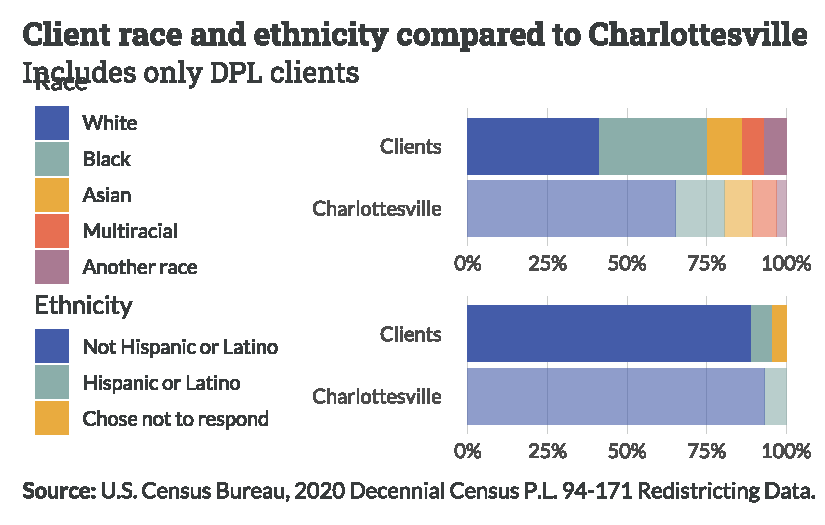
\includegraphics{piedmont_files/figure-pdf/race-ethnicity-1.pdf}

}

\end{figure}

Household incomes are available for 88 of the 131 clients. Of the 43
clients with no income data, all are SPARC-only records. Six of the
eight DPL clients who also used SPARC have two incomes recorded for each
program---these values all differ, sometimes significantly.

\begin{Shaded}
\begin{Highlighting}[]
\CommentTok{\# Summarise clients by household income}

\NormalTok{clients\_inc }\OtherTok{\textless{}{-}}\NormalTok{ clients\_all }\SpecialCharTok{|\textgreater{}} 
  
  \CommentTok{\# Select only id\_pha, program, and income columns}
  
  \FunctionTok{select}\NormalTok{(}\DecValTok{1}\NormalTok{, }\DecValTok{2}\NormalTok{, }\DecValTok{9}\NormalTok{, }\DecValTok{10}\NormalTok{, }\DecValTok{11}\NormalTok{) }\SpecialCharTok{|\textgreater{}} 
  
  \CommentTok{\# Combine DLP and SPARC incomes into one column}
  
  \FunctionTok{mutate}\NormalTok{(}\AttributeTok{income =} \FunctionTok{case\_when}\NormalTok{(}
    \SpecialCharTok{!}\FunctionTok{is.na}\NormalTok{(household\_annual\_income\_dpl) }\SpecialCharTok{\&} \SpecialCharTok{!}\FunctionTok{is.na}\NormalTok{(household\_annual\_income\_spc) }\SpecialCharTok{\textasciitilde{}}\NormalTok{ household\_annual\_income\_dpl,}
    \SpecialCharTok{!}\FunctionTok{is.na}\NormalTok{(household\_annual\_income\_dpl) }\SpecialCharTok{\&} \FunctionTok{is.na}\NormalTok{(household\_annual\_income\_spc) }\SpecialCharTok{\textasciitilde{}}\NormalTok{ household\_annual\_income\_dpl,}
    \FunctionTok{is.na}\NormalTok{(household\_annual\_income\_dpl) }\SpecialCharTok{\&} \SpecialCharTok{!}\FunctionTok{is.na}\NormalTok{(household\_annual\_income\_spc) }\SpecialCharTok{\textasciitilde{}}\NormalTok{ household\_annual\_income\_spc,}
    \ConstantTok{TRUE} \SpecialCharTok{\textasciitilde{}} \ConstantTok{NA\_real\_}
\NormalTok{  )) }\SpecialCharTok{|\textgreater{}} 
  
  \CommentTok{\# Add column describing income data availability}
  
  \FunctionTok{mutate}\NormalTok{(}\AttributeTok{data =} \FunctionTok{case\_when}\NormalTok{(}
    \SpecialCharTok{!}\FunctionTok{is.na}\NormalTok{(household\_annual\_income\_dpl) }\SpecialCharTok{\&} \SpecialCharTok{!}\FunctionTok{is.na}\NormalTok{(household\_annual\_income\_spc) }\SpecialCharTok{\textasciitilde{}} \StringTok{"Different incomes recorded"}\NormalTok{,}
    \SpecialCharTok{!}\FunctionTok{is.na}\NormalTok{(household\_annual\_income\_dpl) }\SpecialCharTok{\&} \FunctionTok{is.na}\NormalTok{(household\_annual\_income\_spc) }\SpecialCharTok{\textasciitilde{}} \StringTok{"Income recorded"}\NormalTok{,}
    \FunctionTok{is.na}\NormalTok{(household\_annual\_income\_dpl) }\SpecialCharTok{\&} \SpecialCharTok{!}\FunctionTok{is.na}\NormalTok{(household\_annual\_income\_spc) }\SpecialCharTok{\textasciitilde{}} \StringTok{"Income recorded"}\NormalTok{,}
    \ConstantTok{TRUE} \SpecialCharTok{\textasciitilde{}} \StringTok{"No data"}
\NormalTok{  )) }

\CommentTok{\# Create plot showing income data availability}

\NormalTok{clients\_inc }\SpecialCharTok{|\textgreater{}} 
  \FunctionTok{group\_by}\NormalTok{(program, data) }\SpecialCharTok{|\textgreater{}} 
  \FunctionTok{summarise}\NormalTok{(}\AttributeTok{n =} \FunctionTok{n}\NormalTok{()) }\SpecialCharTok{|\textgreater{}} 
  \FunctionTok{ggplot}\NormalTok{(}\FunctionTok{aes}\NormalTok{(}\AttributeTok{x =} \FunctionTok{reorder}\NormalTok{(program, n, }\AttributeTok{decreasing =} \ConstantTok{TRUE}\NormalTok{), }\AttributeTok{y =}\NormalTok{ n, }\AttributeTok{fill =}\NormalTok{ data)) }\SpecialCharTok{+}
    \FunctionTok{geom\_col}\NormalTok{(}\AttributeTok{position =} \StringTok{"stack"}\NormalTok{) }\SpecialCharTok{+}
    \FunctionTok{scale\_fill\_hda}\NormalTok{() }\SpecialCharTok{+}
    \FunctionTok{labs}\NormalTok{(}\AttributeTok{title =} \StringTok{"Client income data availability by program"}\NormalTok{,}
         \AttributeTok{subtitle =} \StringTok{"Data from July 2017 through September 2022"}\NormalTok{) }\SpecialCharTok{+}
    \FunctionTok{theme\_hda}\NormalTok{() }\SpecialCharTok{+}
    \FunctionTok{add\_zero\_line}\NormalTok{(}\StringTok{"y"}\NormalTok{) }\SpecialCharTok{+}
    \FunctionTok{theme}\NormalTok{(}
      \AttributeTok{legend.position =} \StringTok{"top"}
\NormalTok{    )}
\end{Highlighting}
\end{Shaded}

\begin{figure}[H]

{\centering 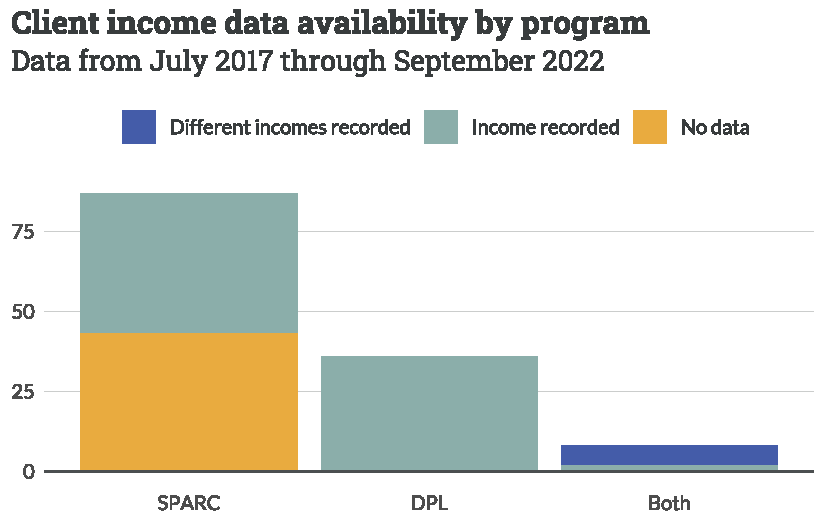
\includegraphics{piedmont_files/figure-pdf/income-data-1.pdf}

}

\end{figure}

Most of PHA's clients have household incomes between \$25,000 and
\$60,000. However, the incomes of SPARC-only clients skew slightly
higher, with some above \$75,000.

\begin{Shaded}
\begin{Highlighting}[]
\CommentTok{\# Summarise income by program}

\FunctionTok{ggplot}\NormalTok{(clients\_inc, }\FunctionTok{aes}\NormalTok{(}\AttributeTok{x =}\NormalTok{ income, }\AttributeTok{y =}\NormalTok{ program, }\AttributeTok{fill =}\NormalTok{ program)) }\SpecialCharTok{+}
  \FunctionTok{geom\_density\_ridges}\NormalTok{(}\AttributeTok{alpha =} \FloatTok{0.9}\NormalTok{) }\SpecialCharTok{+}
  \FunctionTok{scale\_fill\_hda}\NormalTok{() }\SpecialCharTok{+}
  \FunctionTok{scale\_x\_continuous}\NormalTok{(}\AttributeTok{labels =} \FunctionTok{label\_dollar}\NormalTok{()) }\SpecialCharTok{+}
  \FunctionTok{labs}\NormalTok{(}\AttributeTok{title =} \StringTok{"Client household income by program"}\NormalTok{,}
       \AttributeTok{subtitle =} \StringTok{"Data from July 2017 through September 2022"}\NormalTok{,}
       \AttributeTok{caption =} \StringTok{"**Note:** Does not include 43 SPARC clients with no recorded income."}\NormalTok{) }\SpecialCharTok{+}
  \FunctionTok{theme\_hda}\NormalTok{() }\SpecialCharTok{+}
  \FunctionTok{flip\_gridlines}\NormalTok{()}
\end{Highlighting}
\end{Shaded}

\begin{figure}[H]

{\centering 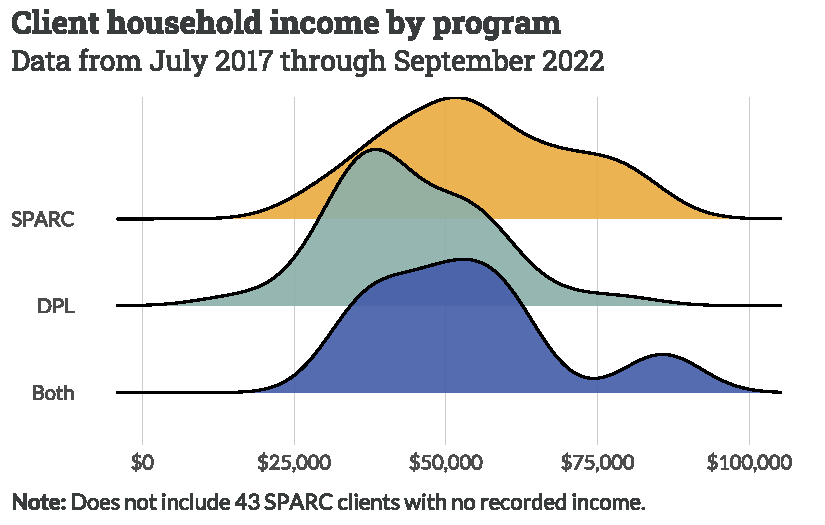
\includegraphics{piedmont_files/figure-pdf/income-plot-1.pdf}

}

\end{figure}

Area median incomes (AMI) are calculated only for clients who used the
DPL program. AMIs are most commonly between 50 and 80 percent, in line
with program eligibility guidelines. On average, AMIs of the DPL clients
who also used SPARC are slightly lower than those of clients who used
DPL only.

\begin{Shaded}
\begin{Highlighting}[]
\CommentTok{\# Summarise AMI by program}

\NormalTok{clients\_inc }\SpecialCharTok{|\textgreater{}} \FunctionTok{filter}\NormalTok{(program }\SpecialCharTok{!=} \StringTok{"SPARC"}\NormalTok{) }\SpecialCharTok{|\textgreater{}} 
\FunctionTok{ggplot}\NormalTok{(}\FunctionTok{aes}\NormalTok{(}\AttributeTok{x =}\NormalTok{ client\_ami, }\AttributeTok{y =}\NormalTok{ program, }\AttributeTok{fill =}\NormalTok{ program)) }\SpecialCharTok{+}
  \FunctionTok{geom\_density\_ridges}\NormalTok{(}\AttributeTok{alpha =} \FloatTok{0.9}\NormalTok{) }\SpecialCharTok{+}
  \FunctionTok{scale\_fill\_hda}\NormalTok{() }\SpecialCharTok{+}
  \FunctionTok{scale\_x\_continuous}\NormalTok{(}\AttributeTok{labels =} \FunctionTok{label\_percent}\NormalTok{(), }\AttributeTok{breaks =} \FunctionTok{c}\NormalTok{(}\DecValTok{0}\NormalTok{, }\FloatTok{0.3}\NormalTok{, }\FloatTok{0.5}\NormalTok{, }\FloatTok{0.6}\NormalTok{, }\FloatTok{0.7}\NormalTok{, }\FloatTok{0.8}\NormalTok{, }\DecValTok{1}\NormalTok{)) }\SpecialCharTok{+}
  \FunctionTok{labs}\NormalTok{(}\AttributeTok{title =} \StringTok{"Client AMI by program"}\NormalTok{,}
       \AttributeTok{subtitle =} \StringTok{"Data from July 2017 through September 2022"}\NormalTok{,}
       \AttributeTok{caption =} \StringTok{"**Note:** Does not include 43 SPARC clients with no recorded income."}\NormalTok{) }\SpecialCharTok{+}
  \FunctionTok{theme\_hda}\NormalTok{() }\SpecialCharTok{+}
  \FunctionTok{flip\_gridlines}\NormalTok{()}
\end{Highlighting}
\end{Shaded}

\begin{figure}[H]

{\centering 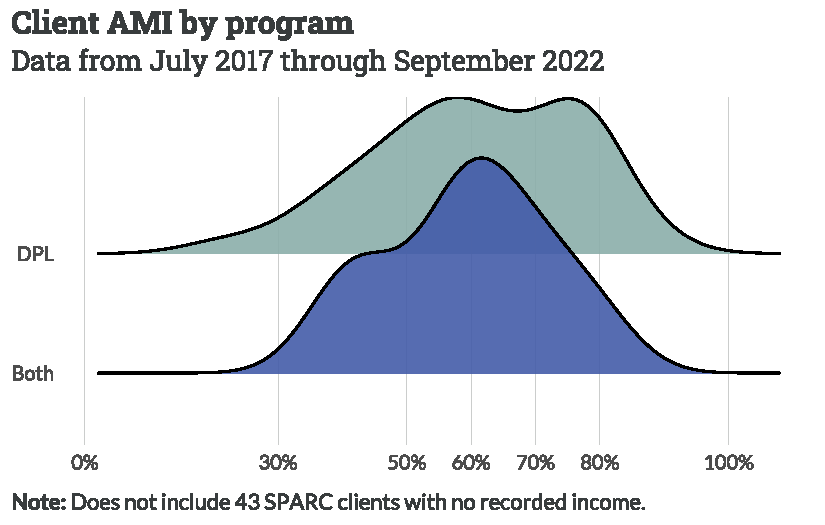
\includegraphics{piedmont_files/figure-pdf/ami-1.pdf}

}

\end{figure}

Compared to the distribution of household incomes in Charlottesville,
clients are much more likely to earn more than most renters, while still
making significantly less than most homeowners. Over 78 percent of
clients earn between \$35,000 and \$75,000, versus just 27 percent of
renters and 20 percent of homeowners.

\begin{Shaded}
\begin{Highlighting}[]
\CommentTok{\# Assign client incomes to ACS categories}

\NormalTok{clients\_inc\_sum }\OtherTok{\textless{}{-}}\NormalTok{ clients\_inc }\SpecialCharTok{|\textgreater{}} 
  \FunctionTok{mutate}\NormalTok{(}\AttributeTok{income =} \FunctionTok{case\_when}\NormalTok{(}
\NormalTok{    income }\SpecialCharTok{\textless{}} \DecValTok{35000} \SpecialCharTok{\textasciitilde{}} \StringTok{"Less than $35,000"}\NormalTok{,}
\NormalTok{    income }\SpecialCharTok{\textgreater{}=} \DecValTok{35000} \SpecialCharTok{\&}\NormalTok{ income }\SpecialCharTok{\textless{}} \DecValTok{50000}  \SpecialCharTok{\textasciitilde{}} \StringTok{"$35,000 to $49,999"}\NormalTok{,}
\NormalTok{    income }\SpecialCharTok{\textgreater{}=} \DecValTok{50000} \SpecialCharTok{\&}\NormalTok{ income }\SpecialCharTok{\textless{}} \DecValTok{75000}  \SpecialCharTok{\textasciitilde{}} \StringTok{"$50,000 to $74,999"}\NormalTok{,}
\NormalTok{    income }\SpecialCharTok{\textgreater{}=} \DecValTok{75000} \SpecialCharTok{\&}\NormalTok{ income }\SpecialCharTok{\textless{}} \DecValTok{100000}  \SpecialCharTok{\textasciitilde{}} \StringTok{"$75,000 to $99,999"}\NormalTok{,}
\NormalTok{    income }\SpecialCharTok{\textgreater{}=} \DecValTok{100000} \SpecialCharTok{\textasciitilde{}} \StringTok{"$100,000 or more"}\NormalTok{,}
    \ConstantTok{TRUE} \SpecialCharTok{\textasciitilde{}} \StringTok{"No data"}
\NormalTok{  )) }\SpecialCharTok{|\textgreater{}} 
  
  \CommentTok{\# Filter out clients with no income data (optional)}
  
  \FunctionTok{filter}\NormalTok{(income }\SpecialCharTok{!=} \StringTok{"No data"}\NormalTok{) }\SpecialCharTok{|\textgreater{}}  
  
  \CommentTok{\# Summarise clients by category}
  
  \FunctionTok{count}\NormalTok{(income) }\SpecialCharTok{|\textgreater{}} 
  
  \CommentTok{\# Get column names to match ACS data}
  
  \FunctionTok{mutate}\NormalTok{(}\AttributeTok{tenure =} \StringTok{"Clients"}\NormalTok{, }\AttributeTok{.before =} \DecValTok{1}\NormalTok{) }\SpecialCharTok{|\textgreater{}} 
  \FunctionTok{rename}\NormalTok{(}\AttributeTok{estimate =}\NormalTok{ n)}

\CommentTok{\# Join ACS income data with client income data}

\NormalTok{clients\_cv\_inc }\OtherTok{\textless{}{-}}\NormalTok{ clients\_inc\_sum }\SpecialCharTok{|\textgreater{}} 
  \FunctionTok{bind\_rows}\NormalTok{(cv\_income) }\SpecialCharTok{|\textgreater{}} 
  
  \CommentTok{\# Add percentages}
  
  \FunctionTok{group\_by}\NormalTok{(tenure) }\SpecialCharTok{|\textgreater{}} 
  \FunctionTok{mutate}\NormalTok{(}\AttributeTok{pct =}\NormalTok{ estimate}\SpecialCharTok{/}\FunctionTok{sum}\NormalTok{(estimate)) }\SpecialCharTok{|\textgreater{}} 
  
  \CommentTok{\# Reorder income categories}
  
  \FunctionTok{mutate}\NormalTok{(}\AttributeTok{income =} \FunctionTok{fct\_relevel}\NormalTok{(}
\NormalTok{    income, }\StringTok{"Less than $35,000"}\NormalTok{, }\StringTok{"$35,000 to $49,999"}\NormalTok{, }\StringTok{"$50,000 to $74,999"}\NormalTok{,}
    \StringTok{"$75,000 to $99,999"}\NormalTok{, }\StringTok{"$100,000 or more"}\NormalTok{))}

\CommentTok{\# Create plot}

\FunctionTok{ggplot}\NormalTok{(clients\_cv\_inc, }\FunctionTok{aes}\NormalTok{(}\AttributeTok{y =}\NormalTok{ pct, }\AttributeTok{x =}\NormalTok{ tenure, }\AttributeTok{fill =}\NormalTok{ tenure)) }\SpecialCharTok{+}
  \FunctionTok{geom\_col}\NormalTok{() }\SpecialCharTok{+}
  \FunctionTok{facet\_wrap}\NormalTok{(}\SpecialCharTok{\textasciitilde{}}\NormalTok{income, }\AttributeTok{nrow =} \DecValTok{1}\NormalTok{, }\AttributeTok{labeller =} \FunctionTok{label\_wrap\_gen}\NormalTok{(}\DecValTok{12}\NormalTok{)) }\SpecialCharTok{+}
  \FunctionTok{scale\_y\_continuous}\NormalTok{(}\AttributeTok{labels =} \FunctionTok{label\_percent}\NormalTok{()) }\SpecialCharTok{+}
  \FunctionTok{scale\_fill\_hda}\NormalTok{() }\SpecialCharTok{+}
  \FunctionTok{labs}\NormalTok{(}\AttributeTok{title =} \StringTok{"Client income compared to Charlottesville"}\NormalTok{,}
       \AttributeTok{subtitle =} \StringTok{"Data from July 2017 through September 2022"}\NormalTok{,}
       \AttributeTok{caption =} \StringTok{"**Source:** U.S. Census Bureau, American Community Survey, 2017{-}2021 5{-}year estimates. Table B25118.\textless{}br\textgreater{}**Note:** Does not include 43 records where client income data not available."}\NormalTok{) }\SpecialCharTok{+}
  \FunctionTok{theme\_hda}\NormalTok{() }\SpecialCharTok{+}
  \FunctionTok{add\_zero\_line}\NormalTok{(}\StringTok{"y"}\NormalTok{) }\SpecialCharTok{+}
  \FunctionTok{theme}\NormalTok{(}\AttributeTok{axis.text.x =} \FunctionTok{element\_blank}\NormalTok{(),}
        \AttributeTok{legend.position =} \StringTok{"top"}\NormalTok{)}
\end{Highlighting}
\end{Shaded}

\begin{figure}[H]

{\centering 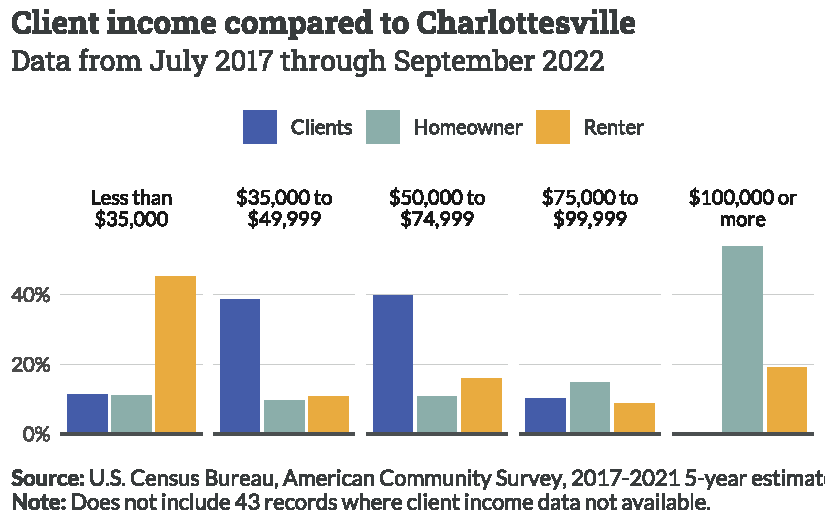
\includegraphics{piedmont_files/figure-pdf/income-compare-1.pdf}

}

\end{figure}

\hypertarget{assistance-levels}{%
\subsection{Assistance levels}\label{assistance-levels}}

PHA's DPL program uses funds from a number of different sources. Clients
were most commonly supported by HOME funds from DHCD (18) and from
Albemarle County's Homebuyer Assistance Program (11). Overall, PHA has
used eight separate sources to fund its DPL program.

\begin{Shaded}
\begin{Highlighting}[]
\NormalTok{dpl\_sources }\OtherTok{\textless{}{-}}\NormalTok{ clients\_all }\SpecialCharTok{|\textgreater{}} 
  \FunctionTok{filter}\NormalTok{(program }\SpecialCharTok{!=} \StringTok{"SPARC"}\NormalTok{) }\SpecialCharTok{|\textgreater{}} 
  \FunctionTok{select}\NormalTok{(}\DecValTok{1}\NormalTok{, }\DecValTok{2}\NormalTok{, }\DecValTok{36}\SpecialCharTok{:}\DecValTok{43}\NormalTok{) }\SpecialCharTok{|\textgreater{}} 
  \FunctionTok{pivot\_longer}\NormalTok{(}
    \AttributeTok{cols =} \FunctionTok{c}\NormalTok{(}\DecValTok{3}\SpecialCharTok{:}\DecValTok{10}\NormalTok{),}
    \AttributeTok{names\_to =} \StringTok{"source"}\NormalTok{,}
    \AttributeTok{values\_to =} \StringTok{"x"}
\NormalTok{  ) }\SpecialCharTok{|\textgreater{}} 
  \FunctionTok{group\_by}\NormalTok{(source) }\SpecialCharTok{|\textgreater{}} 
  \FunctionTok{summarise}\NormalTok{(}\AttributeTok{count =} \FunctionTok{sum}\NormalTok{(x)) }\SpecialCharTok{|\textgreater{}} 
  \FunctionTok{mutate}\NormalTok{(}\AttributeTok{source =} \FunctionTok{case\_when}\NormalTok{(}
\NormalTok{    source }\SpecialCharTok{==} \StringTok{"dhcd"} \SpecialCharTok{\textasciitilde{}} \StringTok{"DHCD HOME"}\NormalTok{,}
\NormalTok{    source }\SpecialCharTok{==} \StringTok{"achap"} \SpecialCharTok{\textasciitilde{}} \StringTok{"Albemarle County HAP"}\NormalTok{,}
\NormalTok{    source }\SpecialCharTok{==} \StringTok{"cdfi"} \SpecialCharTok{\textasciitilde{}} \StringTok{"CDFI Regional Down{-}payment Loan Program"}\NormalTok{,}
\NormalTok{    source }\SpecialCharTok{==} \StringTok{"recycled\_home"} \SpecialCharTok{\textasciitilde{}} \StringTok{"Recycled HOME"}\NormalTok{,}
\NormalTok{    source }\SpecialCharTok{==} \StringTok{"cahf"} \SpecialCharTok{\textasciitilde{}} \StringTok{"Charlottesville Affordable Housing Fund"}\NormalTok{,}
\NormalTok{    source }\SpecialCharTok{==} \StringTok{"city"} \SpecialCharTok{\textasciitilde{}} \StringTok{"Charlottesville HOME"}\NormalTok{,}
\NormalTok{    source }\SpecialCharTok{==} \StringTok{"pha\_regional"} \SpecialCharTok{\textasciitilde{}} \StringTok{"PHA Regional Homeownership Fund"}\NormalTok{,}
\NormalTok{    source }\SpecialCharTok{==} \StringTok{"lchap"} \SpecialCharTok{\textasciitilde{}} \StringTok{"Louisa County HAP"}\NormalTok{,}
    \ConstantTok{TRUE} \SpecialCharTok{\textasciitilde{}} \FunctionTok{str\_to\_upper}\NormalTok{(source)}
\NormalTok{  )) }\SpecialCharTok{|\textgreater{}} 
  \FunctionTok{mutate}\NormalTok{(}\AttributeTok{source =} \FunctionTok{str\_wrap}\NormalTok{(source, }\DecValTok{20}\NormalTok{))}

\FunctionTok{ggplot}\NormalTok{(dpl\_sources, }\FunctionTok{aes}\NormalTok{(}\AttributeTok{x =}\NormalTok{ count, }\AttributeTok{y =} \FunctionTok{reorder}\NormalTok{(source, count), }\AttributeTok{label =}\NormalTok{ count)) }\SpecialCharTok{+} 
  \FunctionTok{geom\_col}\NormalTok{(}\AttributeTok{fill =} \StringTok{"\#445ca9"}\NormalTok{) }\SpecialCharTok{+}
  \FunctionTok{geom\_text}\NormalTok{(}\AttributeTok{color =} \StringTok{"\#FFFFFF"}\NormalTok{, }\AttributeTok{nudge\_x =} \SpecialCharTok{{-}}\FloatTok{0.5}\NormalTok{) }\SpecialCharTok{+}
  \FunctionTok{theme\_hda}\NormalTok{() }\SpecialCharTok{+}
  \FunctionTok{flip\_gridlines}\NormalTok{() }\SpecialCharTok{+}
  \FunctionTok{add\_zero\_line}\NormalTok{(}\StringTok{"x"}\NormalTok{) }\SpecialCharTok{+}
  \FunctionTok{labs}\NormalTok{(}
    \AttributeTok{title =} \StringTok{"Number of DPL awards by source"}\NormalTok{,}
    \AttributeTok{subtitle =} \StringTok{"Data from July 2017 through September 2022"}\NormalTok{,}
    \AttributeTok{caption =} \StringTok{"**Notes:** \textquotesingle{}HAP\textquotesingle{} = Homebuyer Assistance Program."}
\NormalTok{  )}
\end{Highlighting}
\end{Shaded}

\begin{figure}[H]

{\centering 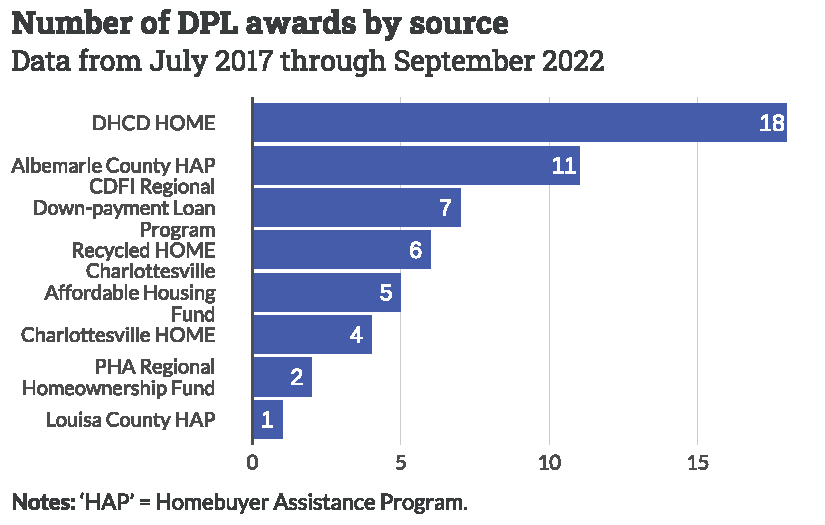
\includegraphics{piedmont_files/figure-pdf/dpl-sources-1.pdf}

}

\end{figure}

PHA awarded a total of \$1,242,190 in DPL assistance from July 2017 to
September 2022. This amounted to roughly \$28,230 provided per client.

\begin{Shaded}
\begin{Highlighting}[]
\NormalTok{dpl\_amount }\OtherTok{\textless{}{-}}\NormalTok{ clients\_all }\SpecialCharTok{|\textgreater{}} 
  \FunctionTok{drop\_na}\NormalTok{(}\StringTok{"close\_date\_dpl"}\NormalTok{) }\SpecialCharTok{|\textgreater{}} 
  \FunctionTok{arrange}\NormalTok{(close\_date\_dpl) }\SpecialCharTok{|\textgreater{}} 
  \FunctionTok{mutate}\NormalTok{(}\AttributeTok{cum\_sum =} \FunctionTok{cumsum}\NormalTok{(pha\_loans\_amount))}

\FunctionTok{ggplot}\NormalTok{(dpl\_amount, }\FunctionTok{aes}\NormalTok{(}\AttributeTok{x =}\NormalTok{ close\_date\_dpl, }\AttributeTok{y =}\NormalTok{ cum\_sum)) }\SpecialCharTok{+}
  \FunctionTok{geom\_area}\NormalTok{(}\AttributeTok{fill =} \StringTok{"\#445ca9"}\NormalTok{) }\SpecialCharTok{+}
  \FunctionTok{scale\_y\_continuous}\NormalTok{(}\AttributeTok{labels =} \FunctionTok{label\_dollar}\NormalTok{(}\AttributeTok{scale =} \FloatTok{0.001}\NormalTok{, }\AttributeTok{suffix =} \StringTok{"k"}\NormalTok{)) }\SpecialCharTok{+}
  \FunctionTok{add\_zero\_line}\NormalTok{(}\StringTok{"y"}\NormalTok{) }\SpecialCharTok{+}
  \FunctionTok{theme\_hda}\NormalTok{() }\SpecialCharTok{+}
  \FunctionTok{labs}\NormalTok{(}
    \AttributeTok{title =} \StringTok{"Total amount of DPL assistance awarded"}\NormalTok{,}
    \AttributeTok{subtitle =} \StringTok{"Data from July 2017 through September 2022"}
\NormalTok{  )}
\end{Highlighting}
\end{Shaded}

\begin{figure}[H]

{\centering 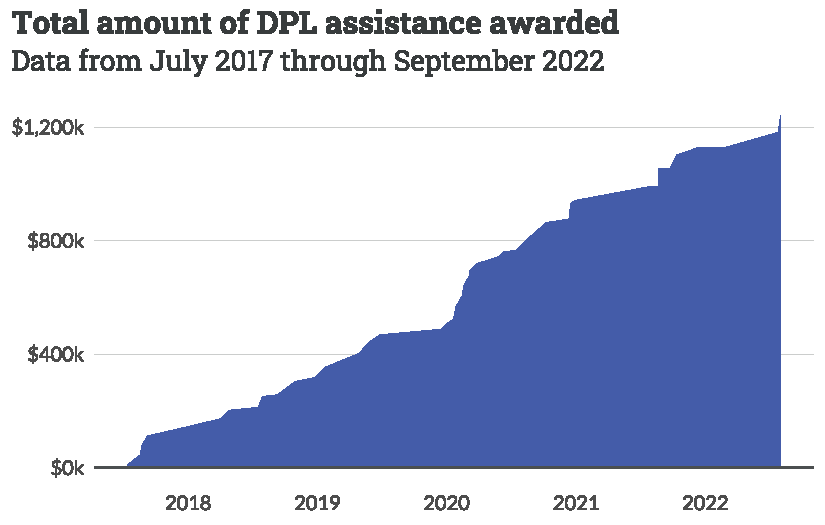
\includegraphics{piedmont_files/figure-pdf/dpl-amount-1.pdf}

}

\end{figure}

The average amount each client received stayed around \$28,000 from 2017
through 2020. In 2021, that average increased to \$37,435. In 2022, the
two clients that received DPL each received significant DPL assistance
well above prior year averages.

\begin{Shaded}
\begin{Highlighting}[]
\NormalTok{dpl\_annual }\OtherTok{\textless{}{-}}\NormalTok{ dpl\_amount }\SpecialCharTok{|\textgreater{}} 
  \FunctionTok{mutate}\NormalTok{(}\AttributeTok{year =} \FunctionTok{format}\NormalTok{(close\_date\_dpl, }\AttributeTok{format =} \StringTok{"\%Y"}\NormalTok{)) }\SpecialCharTok{|\textgreater{}} 
  \FunctionTok{filter}\NormalTok{(pha\_loans\_amount }\SpecialCharTok{!=} \DecValTok{0}\NormalTok{) }\SpecialCharTok{|\textgreater{}} 
  \FunctionTok{group\_by}\NormalTok{(year) }\SpecialCharTok{|\textgreater{}} 
  \FunctionTok{summarise}\NormalTok{(}\AttributeTok{avg =} \FunctionTok{mean}\NormalTok{(pha\_loans\_amount),}
            \AttributeTok{clients =} \FunctionTok{n}\NormalTok{())}

\FunctionTok{ggplot}\NormalTok{(dpl\_annual, }\FunctionTok{aes}\NormalTok{(}\AttributeTok{x =}\NormalTok{ year, }\AttributeTok{y =}\NormalTok{ avg, }\AttributeTok{label =}\NormalTok{ clients)) }\SpecialCharTok{+}
  \FunctionTok{geom\_col}\NormalTok{(}\AttributeTok{fill =} \StringTok{"\#445ca9"}\NormalTok{) }\SpecialCharTok{+}
  \FunctionTok{geom\_text}\NormalTok{(}\AttributeTok{vjust =} \DecValTok{2}\NormalTok{,}
            \AttributeTok{color =} \StringTok{"white"}\NormalTok{,}
            \AttributeTok{size =} \DecValTok{5}\NormalTok{) }\SpecialCharTok{+}
  \FunctionTok{scale\_y\_continuous}\NormalTok{(}\AttributeTok{labels =} \FunctionTok{label\_dollar}\NormalTok{(}\AttributeTok{scale =} \FloatTok{0.001}\NormalTok{, }\AttributeTok{suffix =} \StringTok{"k"}\NormalTok{),}
                     \AttributeTok{breaks =} \FunctionTok{c}\NormalTok{(}\DecValTok{10000}\NormalTok{, }\DecValTok{20000}\NormalTok{, }\DecValTok{30000}\NormalTok{, }\DecValTok{40000}\NormalTok{, }\DecValTok{50000}\NormalTok{)) }\SpecialCharTok{+}
  \FunctionTok{add\_zero\_line}\NormalTok{(}\StringTok{"y"}\NormalTok{) }\SpecialCharTok{+}
  \FunctionTok{theme\_hda}\NormalTok{() }\SpecialCharTok{+}
  \FunctionTok{labs}\NormalTok{(}
    \AttributeTok{title =} \StringTok{"Average amount of DPL assistance awarded per client"}\NormalTok{,}
    \AttributeTok{subtitle =} \StringTok{"Data from July 2017 through September 2022"}\NormalTok{,}
    \AttributeTok{caption =} \StringTok{"**Note:** Bars show total number of clients for that group."}
\NormalTok{  )}
\end{Highlighting}
\end{Shaded}

\begin{figure}[H]

{\centering 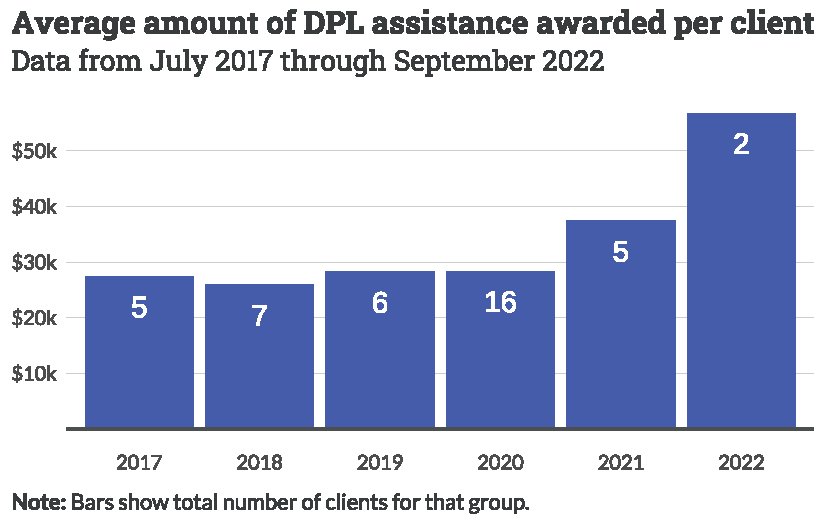
\includegraphics{piedmont_files/figure-pdf/dpl-annual-1.pdf}

}

\end{figure}

Black clients were the only race with an average DPL amount (\$20,761)
below the overall average. Asian, Black and White, and White-alone
clients all had averages between \$32,000 and \$34,000. Three clients of
another race tallied a notably higher average at \$42,973.

\begin{Shaded}
\begin{Highlighting}[]
\NormalTok{dpl\_race }\OtherTok{\textless{}{-}}\NormalTok{ dpl\_amount }\SpecialCharTok{|\textgreater{}} 
  \FunctionTok{filter}\NormalTok{(pha\_loans\_amount }\SpecialCharTok{!=} \DecValTok{0}\NormalTok{) }\SpecialCharTok{|\textgreater{}} 
  \FunctionTok{group\_by}\NormalTok{(race) }\SpecialCharTok{|\textgreater{}} 
  \FunctionTok{summarise}\NormalTok{(}\AttributeTok{avg =} \FunctionTok{mean}\NormalTok{(pha\_loans\_amount),}
            \AttributeTok{clients =} \FunctionTok{n}\NormalTok{())}

\FunctionTok{ggplot}\NormalTok{(dpl\_race, }\FunctionTok{aes}\NormalTok{(}\AttributeTok{x =} \FunctionTok{reorder}\NormalTok{(race, avg), }\AttributeTok{y =}\NormalTok{ avg, }\AttributeTok{fill =}\NormalTok{ race, }\AttributeTok{label =}\NormalTok{ clients)) }\SpecialCharTok{+}
  \FunctionTok{geom\_col}\NormalTok{() }\SpecialCharTok{+}
  \FunctionTok{geom\_text}\NormalTok{(}\AttributeTok{vjust =} \DecValTok{2}\NormalTok{,}
            \AttributeTok{color =} \StringTok{"white"}\NormalTok{,}
            \AttributeTok{size =} \DecValTok{5}\NormalTok{) }\SpecialCharTok{+}
  \FunctionTok{scale\_fill\_hda}\NormalTok{() }\SpecialCharTok{+}
  \FunctionTok{scale\_y\_continuous}\NormalTok{(}\AttributeTok{labels =} \FunctionTok{label\_dollar}\NormalTok{(}\AttributeTok{scale =} \FloatTok{0.001}\NormalTok{, }\AttributeTok{suffix =} \StringTok{"k"}\NormalTok{),}
                     \AttributeTok{breaks =} \FunctionTok{c}\NormalTok{(}\DecValTok{10000}\NormalTok{, }\DecValTok{20000}\NormalTok{, }\DecValTok{30000}\NormalTok{, }\DecValTok{40000}\NormalTok{, }\DecValTok{50000}\NormalTok{)) }\SpecialCharTok{+}
  \FunctionTok{add\_zero\_line}\NormalTok{(}\StringTok{"y"}\NormalTok{) }\SpecialCharTok{+}
  \FunctionTok{theme\_hda}\NormalTok{() }\SpecialCharTok{+}
  \FunctionTok{labs}\NormalTok{(}
    \AttributeTok{title =} \StringTok{"Average amount of DPL assistance awarded by race"}\NormalTok{,}
    \AttributeTok{subtitle =} \StringTok{"Data from July 2017 through September 2022"}\NormalTok{,}
    \AttributeTok{caption =} \StringTok{"**Note:** Bars show total number of clients for that group."}
\NormalTok{  )}
\end{Highlighting}
\end{Shaded}

\begin{figure}[H]

{\centering 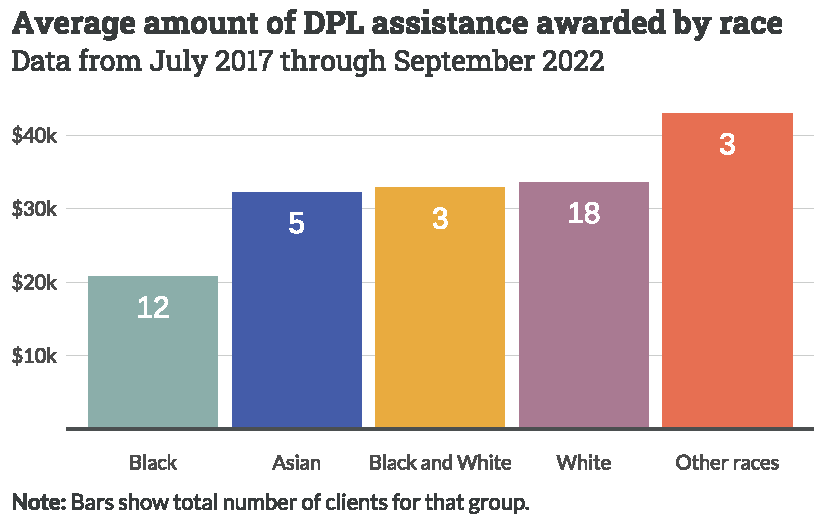
\includegraphics{piedmont_files/figure-pdf/dpl-race-1.pdf}

}

\end{figure}

Only five total clients were Hispanic or chose not to respond when asked
their ethnicity. As a result, the average DPL amount for non-Hispanic
clients (\$29,310) is very close to the overall client average. Among
the three clients who were Hispanic, their average DPL amounted to a
much larger \$42,316.

\begin{Shaded}
\begin{Highlighting}[]
\NormalTok{dpl\_ethnicity }\OtherTok{\textless{}{-}}\NormalTok{ dpl\_amount }\SpecialCharTok{|\textgreater{}} 
  \FunctionTok{filter}\NormalTok{(pha\_loans\_amount }\SpecialCharTok{!=} \DecValTok{0}\NormalTok{) }\SpecialCharTok{|\textgreater{}} 
  \FunctionTok{group\_by}\NormalTok{(ethnicity) }\SpecialCharTok{|\textgreater{}} 
  \FunctionTok{summarise}\NormalTok{(}\AttributeTok{avg =} \FunctionTok{mean}\NormalTok{(pha\_loans\_amount),}
            \AttributeTok{clients =} \FunctionTok{n}\NormalTok{())}

\FunctionTok{ggplot}\NormalTok{(dpl\_ethnicity, }\FunctionTok{aes}\NormalTok{(}\AttributeTok{x =} \FunctionTok{reorder}\NormalTok{(ethnicity, avg), }\AttributeTok{y =}\NormalTok{ avg, }\AttributeTok{fill =}\NormalTok{ ethnicity, }\AttributeTok{label =}\NormalTok{ clients)) }\SpecialCharTok{+}
  \FunctionTok{geom\_col}\NormalTok{() }\SpecialCharTok{+}
  \FunctionTok{geom\_text}\NormalTok{(}\AttributeTok{vjust =} \DecValTok{2}\NormalTok{,}
            \AttributeTok{color =} \StringTok{"white"}\NormalTok{,}
            \AttributeTok{size =} \DecValTok{5}\NormalTok{) }\SpecialCharTok{+}
  \FunctionTok{scale\_fill\_hda}\NormalTok{() }\SpecialCharTok{+}
  \FunctionTok{scale\_y\_continuous}\NormalTok{(}\AttributeTok{labels =} \FunctionTok{label\_dollar}\NormalTok{(}\AttributeTok{scale =} \FloatTok{0.001}\NormalTok{, }\AttributeTok{suffix =} \StringTok{"k"}\NormalTok{),}
                     \AttributeTok{breaks =} \FunctionTok{c}\NormalTok{(}\DecValTok{10000}\NormalTok{, }\DecValTok{20000}\NormalTok{, }\DecValTok{30000}\NormalTok{, }\DecValTok{40000}\NormalTok{, }\DecValTok{50000}\NormalTok{)) }\SpecialCharTok{+}
  \FunctionTok{add\_zero\_line}\NormalTok{(}\StringTok{"y"}\NormalTok{) }\SpecialCharTok{+}
  \FunctionTok{theme\_hda}\NormalTok{() }\SpecialCharTok{+}
  \FunctionTok{labs}\NormalTok{(}
    \AttributeTok{title =} \StringTok{"Average amount of DPL assistance awarded by ethnicity"}\NormalTok{,}
    \AttributeTok{subtitle =} \StringTok{"Data from July 2017 through September 2022"}\NormalTok{,}
    \AttributeTok{caption =} \StringTok{"**Note:** Bars show total number of clients for that group."}
\NormalTok{  )}
\end{Highlighting}
\end{Shaded}

\begin{figure}[H]

{\centering 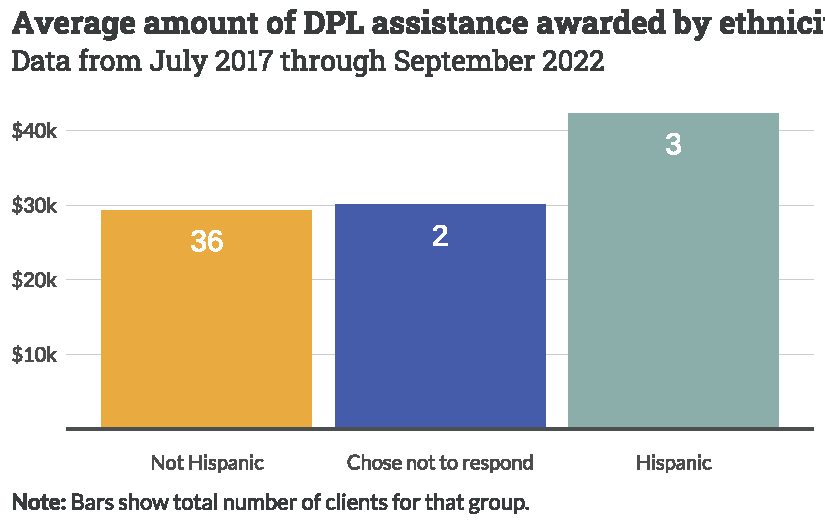
\includegraphics{piedmont_files/figure-pdf/dpl-ethnicity-1.pdf}

}

\end{figure}

\hypertarget{spatial-patterns}{%
\subsection{Spatial patterns}\label{spatial-patterns}}

\begin{tcolorbox}[enhanced jigsaw, coltitle=black, titlerule=0mm, breakable, colbacktitle=quarto-callout-warning-color!10!white, opacityback=0, leftrule=.75mm, opacitybacktitle=0.6, rightrule=.15mm, title=\textcolor{quarto-callout-warning-color}{\faExclamationTriangle}\hspace{0.5em}{Note}, arc=.35mm, colback=white, bottomtitle=1mm, toptitle=1mm, colframe=quarto-callout-warning-color-frame, bottomrule=.15mm, toprule=.15mm, left=2mm]

Client and property location data is only available for clients who used
the DPL program.

\end{tcolorbox}

\begin{Shaded}
\begin{Highlighting}[]
\CommentTok{\# Get list of all localities in Virginia}

\NormalTok{va\_localities }\OtherTok{\textless{}{-}} \FunctionTok{list\_counties}\NormalTok{(}\StringTok{"VA"}\NormalTok{)}

\CommentTok{\# Get all census tracts for Virginia}

\NormalTok{va\_tracts }\OtherTok{\textless{}{-}} \FunctionTok{tracts}\NormalTok{(}\AttributeTok{state =} \StringTok{"VA"}\NormalTok{) }\SpecialCharTok{|\textgreater{}} 
  \FunctionTok{left\_join}\NormalTok{(va\_localities, }\AttributeTok{by =} \FunctionTok{c}\NormalTok{(}\StringTok{"COUNTYFP"} \OtherTok{=} \StringTok{"county\_code"}\NormalTok{)) }\SpecialCharTok{|\textgreater{}} 
  \FunctionTok{st\_transform}\NormalTok{(}\DecValTok{4502}\NormalTok{)}

\CommentTok{\# Geocode client addresses}

\NormalTok{clients\_geocode }\OtherTok{\textless{}{-}}\NormalTok{ clients\_all }\SpecialCharTok{|\textgreater{}} 
  \FunctionTok{geocode}\NormalTok{(}\AttributeTok{street =}\NormalTok{ client\_street\_address, }\AttributeTok{state =}\NormalTok{ client\_state,}
          \AttributeTok{city =}\NormalTok{ client\_city, }\AttributeTok{postalcode =}\NormalTok{ client\_zip,}
          \AttributeTok{method =} \StringTok{"geocodio"}\NormalTok{,}
          \AttributeTok{lat =}\NormalTok{ lat,}
          \AttributeTok{long =}\NormalTok{ long) }\SpecialCharTok{|\textgreater{}} 
  
  \CommentTok{\# Drop SPARC entries with no address data}
  
  \FunctionTok{drop\_na}\NormalTok{(lat) }\SpecialCharTok{|\textgreater{}} 
  
  \CommentTok{\# Specify WGS 1984 coordinate system for lat/long data}
  
  \FunctionTok{st\_as\_sf}\NormalTok{(}\AttributeTok{coords =} \FunctionTok{c}\NormalTok{(}\StringTok{"long"}\NormalTok{, }\StringTok{"lat"}\NormalTok{),}
           \AttributeTok{remove =} \ConstantTok{FALSE}\NormalTok{,}
           \AttributeTok{crs =} \DecValTok{4326}\NormalTok{) }\SpecialCharTok{|\textgreater{}} 
  
  \CommentTok{\# Project into Virginia State Plane South}
  
  \FunctionTok{st\_transform}\NormalTok{(}\DecValTok{4502}\NormalTok{)}

\CommentTok{\# Spatial join client data with tracts and localities}
  
\NormalTok{clients\_sf }\OtherTok{\textless{}{-}} \FunctionTok{st\_join}\NormalTok{(clients\_geocode, va\_tracts) }\SpecialCharTok{|\textgreater{}} 
  \FunctionTok{rename}\NormalTok{(}\AttributeTok{Locality =}\NormalTok{ county)}
  
\CommentTok{\# Geocode property addresses}
  
\NormalTok{property\_geocode }\OtherTok{\textless{}{-}}\NormalTok{ clients\_all }\SpecialCharTok{|\textgreater{}}
  \FunctionTok{geocode}\NormalTok{(}\AttributeTok{street =}\NormalTok{ property\_street\_address, }\AttributeTok{state =}\NormalTok{ property\_state,}
          \AttributeTok{city =}\NormalTok{ property\_city, }\AttributeTok{postalcode =}\NormalTok{ property\_zip,}
          \AttributeTok{method =} \StringTok{"geocodio"}\NormalTok{,}
          \AttributeTok{lat =}\NormalTok{ lat,}
          \AttributeTok{long =}\NormalTok{ long) }\SpecialCharTok{|\textgreater{}} 
  
  \CommentTok{\# Drop SPARC entries with no address data}
  
  \FunctionTok{drop\_na}\NormalTok{(lat) }\SpecialCharTok{|\textgreater{}} 
  
  \CommentTok{\# Specify WGS 1984 coordinate system for lat/long data}
  
  \FunctionTok{st\_as\_sf}\NormalTok{(}\AttributeTok{coords =} \FunctionTok{c}\NormalTok{(}\StringTok{"long"}\NormalTok{, }\StringTok{"lat"}\NormalTok{),}
           \AttributeTok{remove =} \ConstantTok{FALSE}\NormalTok{,}
           \AttributeTok{crs =} \DecValTok{4326}\NormalTok{) }\SpecialCharTok{|\textgreater{}} 
  
  \CommentTok{\# Project into Virginia State Plane South}
  
  \FunctionTok{st\_transform}\NormalTok{(}\DecValTok{4502}\NormalTok{)}

\CommentTok{\# Spatial join client data with tracts and localities}
  
\NormalTok{property\_sf }\OtherTok{\textless{}{-}} \FunctionTok{st\_join}\NormalTok{(property\_geocode, va\_tracts) }\SpecialCharTok{|\textgreater{}} 
  \FunctionTok{rename}\NormalTok{(}\AttributeTok{Locality =}\NormalTok{ county)}

\CommentTok{\# Save data}

\FunctionTok{write\_rds}\NormalTok{(clients\_sf, }\StringTok{"data/clients\_sf.rds"}\NormalTok{)}
\FunctionTok{write\_rds}\NormalTok{(property\_sf, }\StringTok{"data/property\_sf.rds"}\NormalTok{)}
\end{Highlighting}
\end{Shaded}

\hypertarget{client-origins}{%
\subsubsection{Client origins}\label{client-origins}}

The map below shows the original addresses of each client, i.e.~where
they lived when they applied for DPL assistance.

\begin{Shaded}
\begin{Highlighting}[]
\CommentTok{\# Make map of clients}

\NormalTok{clients\_sf }\OtherTok{\textless{}{-}} \FunctionTok{read\_rds}\NormalTok{(}\StringTok{"data/clients\_sf.rds"}\NormalTok{)}

\FunctionTok{mapview}\NormalTok{(}
\NormalTok{  clients\_sf,}
  \AttributeTok{zcol =} \StringTok{"Locality"}\NormalTok{,}
  \AttributeTok{layer.name =} \StringTok{"Client locality"}\NormalTok{,}
  \AttributeTok{label =} \ConstantTok{FALSE}\NormalTok{,}
  \AttributeTok{popup =} \ConstantTok{FALSE}
\NormalTok{)}
\end{Highlighting}
\end{Shaded}

\begin{figure}[H]

{\centering 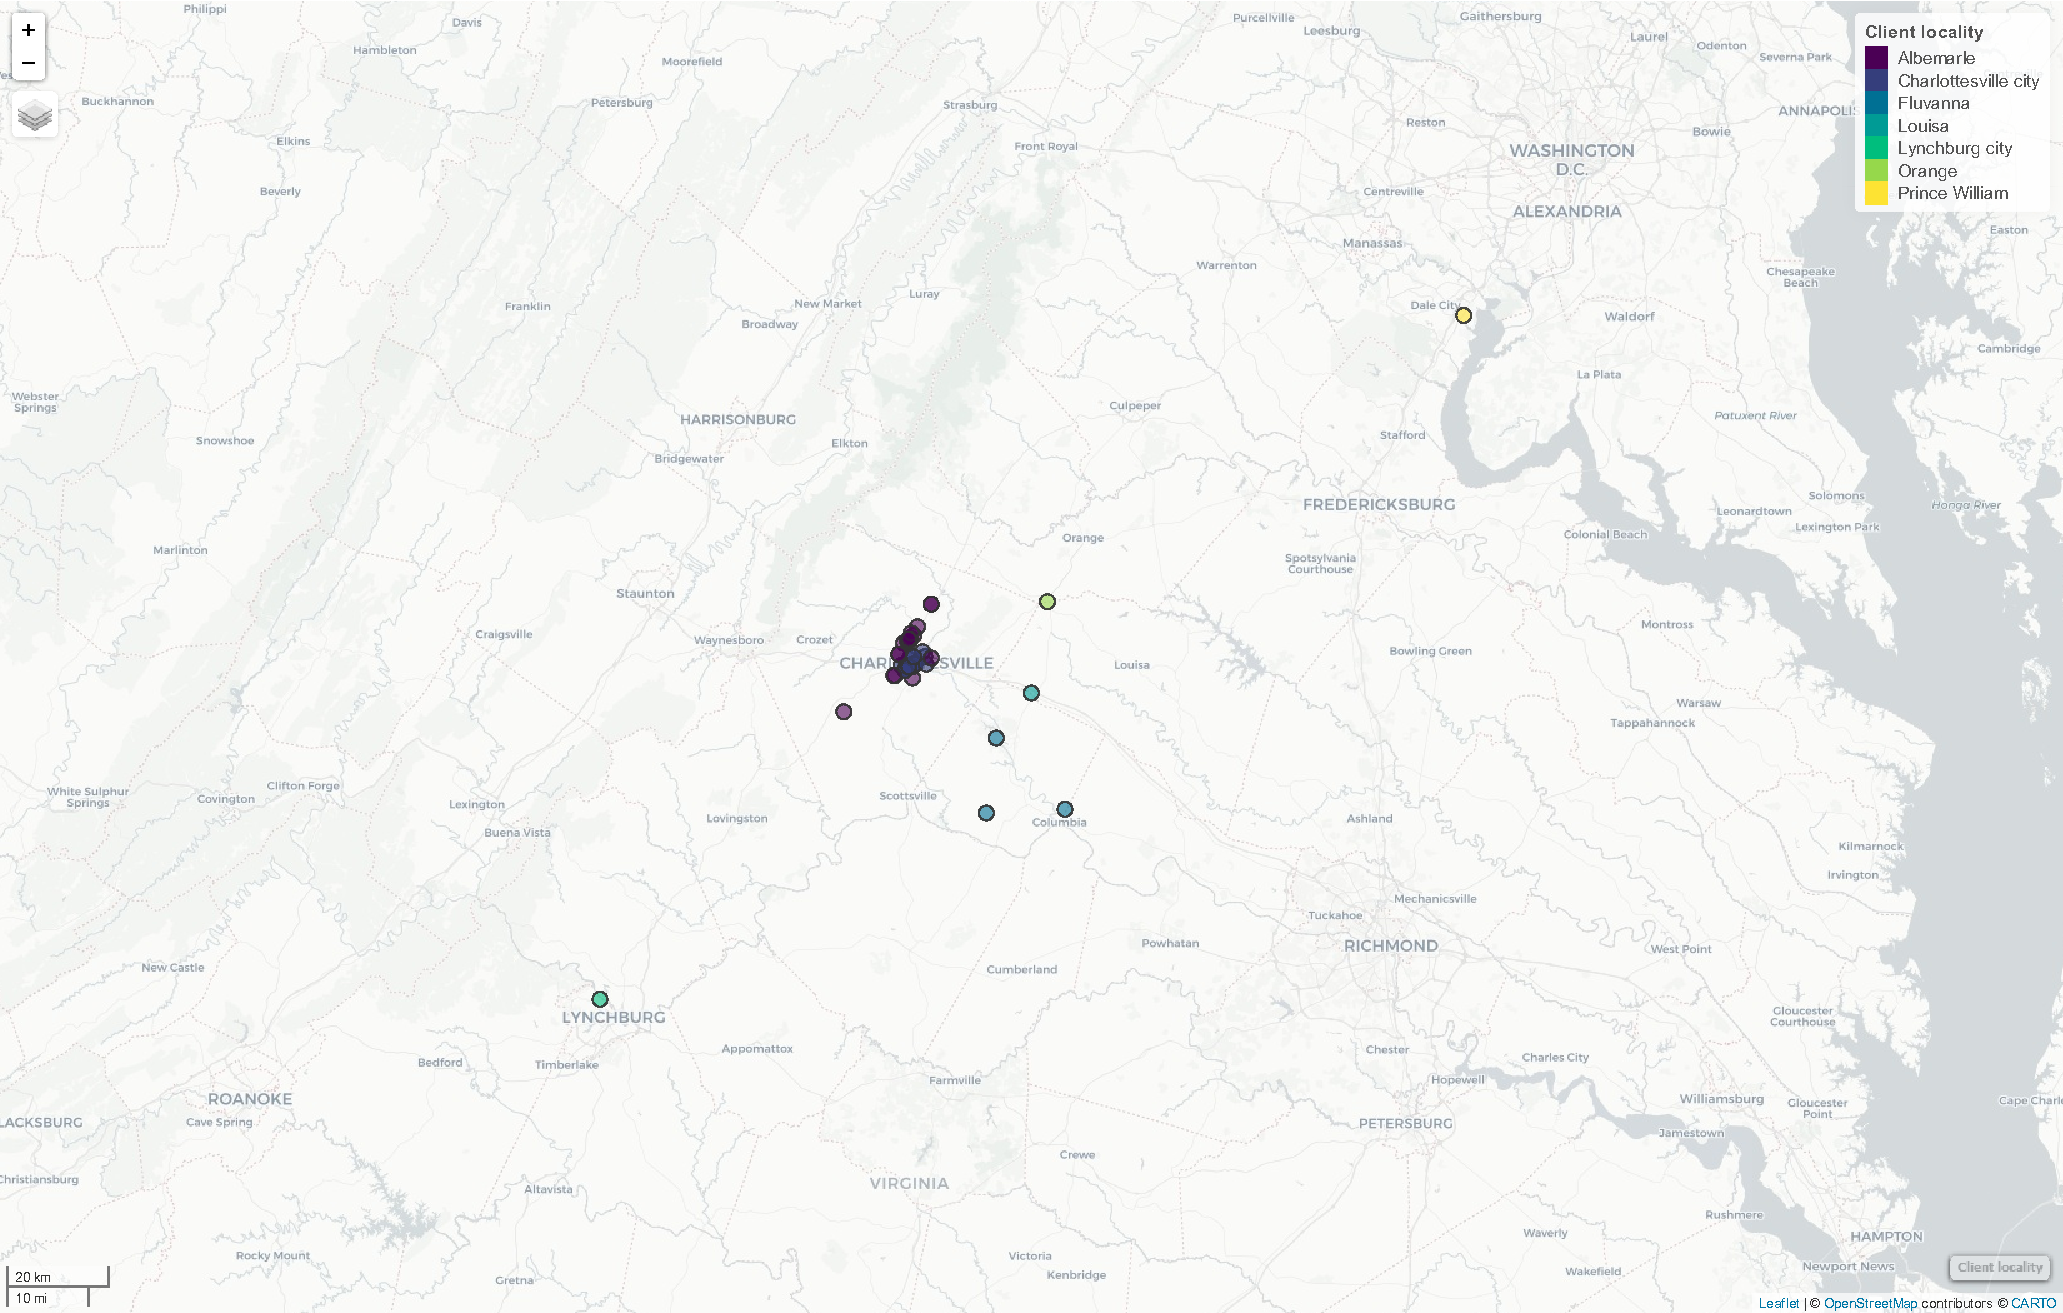
\includegraphics{piedmont_files/figure-pdf/clients-map-1.pdf}

}

\end{figure}

Most clients lived in either Albemarle (20) or Charlottesville (17) when
they applied to the DPL program. Three clients also came from Fluvanna,
while all other origin localities has one client each.

\begin{Shaded}
\begin{Highlighting}[]
\NormalTok{clients\_locality }\OtherTok{\textless{}{-}}\NormalTok{ clients\_sf }\SpecialCharTok{|\textgreater{}} 
  \FunctionTok{count}\NormalTok{(Locality)}

\FunctionTok{ggplot}\NormalTok{(clients\_locality, }\FunctionTok{aes}\NormalTok{(}\AttributeTok{x =}\NormalTok{ n, }\AttributeTok{y =} \FunctionTok{reorder}\NormalTok{(Locality, n), }\AttributeTok{label =}\NormalTok{ n)) }\SpecialCharTok{+}
  \FunctionTok{geom\_col}\NormalTok{(}\AttributeTok{fill =} \StringTok{"\#445ca9"}\NormalTok{) }\SpecialCharTok{+}
  \FunctionTok{geom\_text}\NormalTok{(}\AttributeTok{color =} \StringTok{"\#FFFFFF"}\NormalTok{, }\AttributeTok{nudge\_x =} \SpecialCharTok{{-}}\FloatTok{0.5}\NormalTok{) }\SpecialCharTok{+}
  \FunctionTok{theme\_hda}\NormalTok{() }\SpecialCharTok{+}
  \FunctionTok{flip\_gridlines}\NormalTok{() }\SpecialCharTok{+}
  \FunctionTok{add\_zero\_line}\NormalTok{(}\StringTok{"x"}\NormalTok{) }\SpecialCharTok{+}
  \FunctionTok{labs}\NormalTok{(}
    \AttributeTok{title =} \StringTok{"Number of clients by locality of origin"}\NormalTok{,}
    \AttributeTok{subtitle =} \StringTok{"Data from July 2017 through September 2022"}
\NormalTok{  )}
\end{Highlighting}
\end{Shaded}

\begin{figure}[H]

{\centering 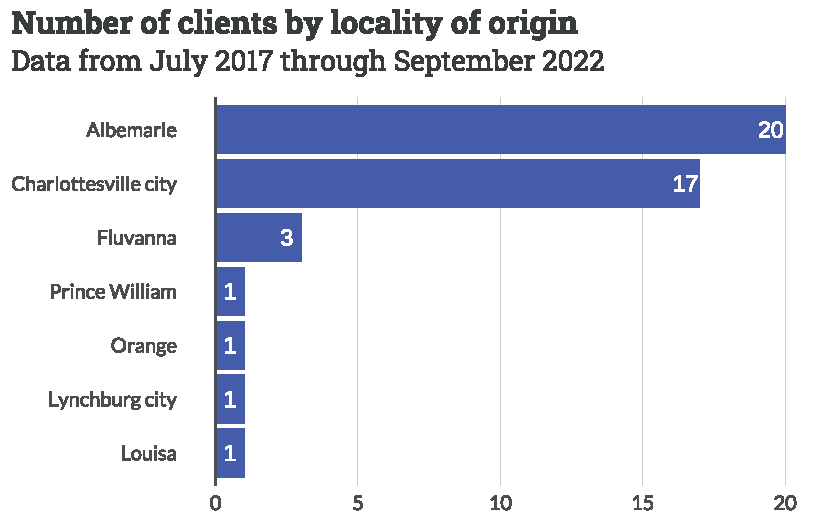
\includegraphics{piedmont_files/figure-pdf/clients-locality-1.pdf}

}

\end{figure}

\hypertarget{client-destinations}{%
\subsubsection{Client destinations}\label{client-destinations}}

The map below shows the addresses of homes purchased by clients,
i.e.~where they moved after using the DPL program.

\begin{Shaded}
\begin{Highlighting}[]
\CommentTok{\# Make map of properties}

\NormalTok{property\_sf }\OtherTok{\textless{}{-}} \FunctionTok{read\_rds}\NormalTok{(}\StringTok{"data/property\_sf.rds"}\NormalTok{)}

\FunctionTok{mapview}\NormalTok{(}
\NormalTok{  property\_sf,}
  \AttributeTok{zcol =} \StringTok{"Locality"}\NormalTok{,}
  \AttributeTok{layer.name =} \StringTok{"Property locality"}\NormalTok{,}
  \AttributeTok{label =} \ConstantTok{FALSE}\NormalTok{,}
  \AttributeTok{popup =} \ConstantTok{FALSE}
\NormalTok{)}
\end{Highlighting}
\end{Shaded}

\begin{figure}[H]

{\centering 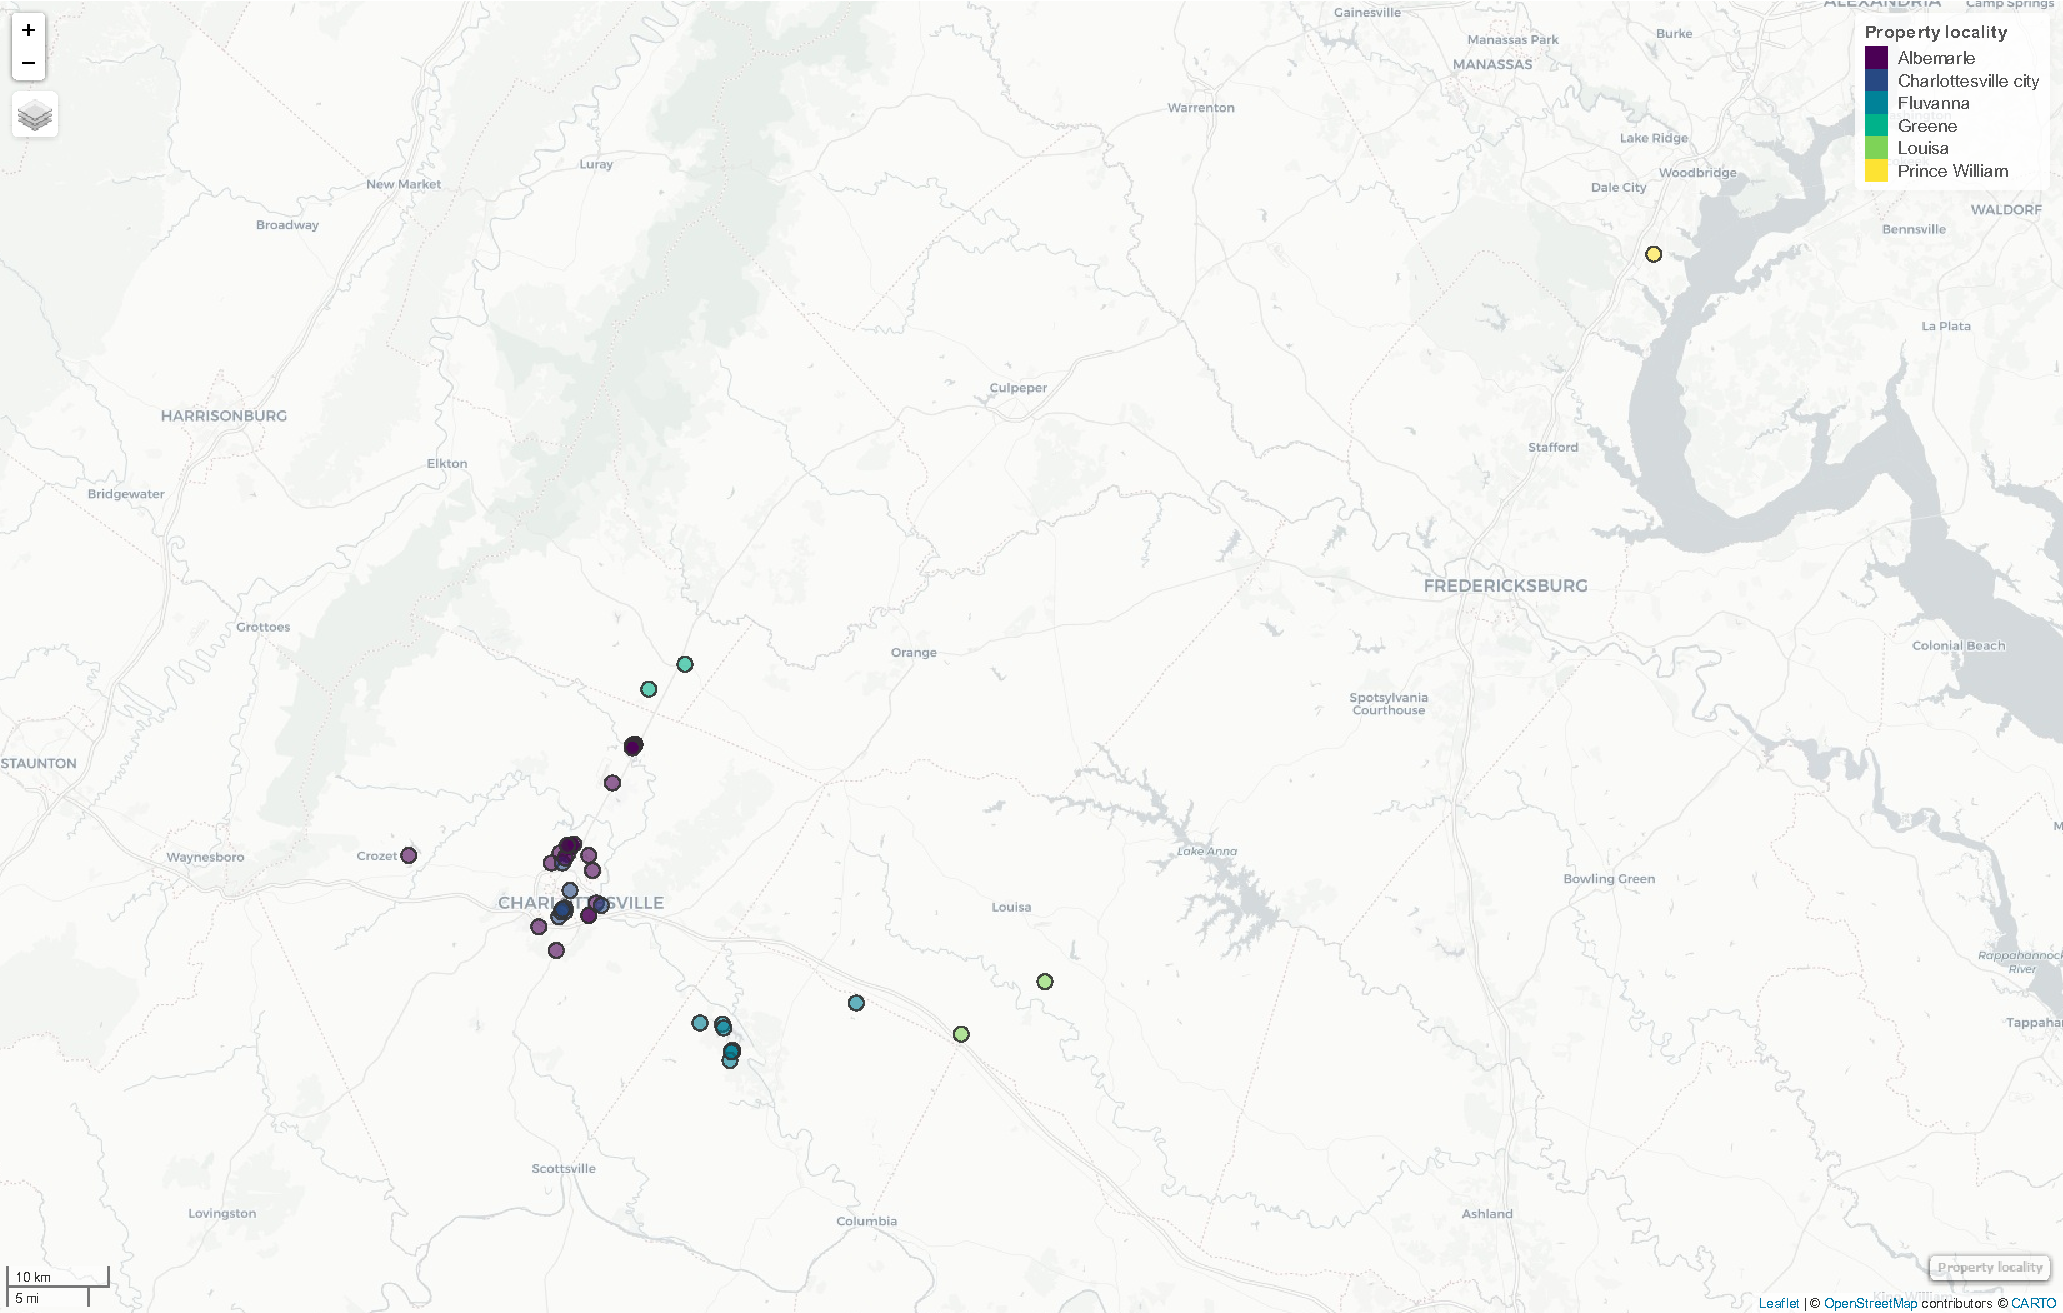
\includegraphics{piedmont_files/figure-pdf/property-map-1.pdf}

}

\end{figure}

The majority of homes purchased by clients were in Albemarle (22),
followed by Charlottesville (9) and Fluvanna (8). Two or fewer clients
purchased homes in each of the other localities.

\begin{Shaded}
\begin{Highlighting}[]
\NormalTok{property\_locality }\OtherTok{\textless{}{-}}\NormalTok{ property\_sf }\SpecialCharTok{|\textgreater{}} 
  \FunctionTok{count}\NormalTok{(Locality)}

\FunctionTok{ggplot}\NormalTok{(property\_locality, }\FunctionTok{aes}\NormalTok{(}\AttributeTok{x =}\NormalTok{ n, }\AttributeTok{y =} \FunctionTok{reorder}\NormalTok{(Locality, n), }\AttributeTok{label =}\NormalTok{ n)) }\SpecialCharTok{+}
  \FunctionTok{geom\_col}\NormalTok{(}\AttributeTok{fill =} \StringTok{"\#445ca9"}\NormalTok{) }\SpecialCharTok{+}
  \FunctionTok{geom\_text}\NormalTok{(}\AttributeTok{color =} \StringTok{"\#FFFFFF"}\NormalTok{, }\AttributeTok{nudge\_x =} \SpecialCharTok{{-}}\FloatTok{0.5}\NormalTok{) }\SpecialCharTok{+}
  \FunctionTok{theme\_hda}\NormalTok{() }\SpecialCharTok{+}
  \FunctionTok{flip\_gridlines}\NormalTok{() }\SpecialCharTok{+}
  \FunctionTok{add\_zero\_line}\NormalTok{(}\StringTok{"x"}\NormalTok{) }\SpecialCharTok{+}
  \FunctionTok{labs}\NormalTok{(}
    \AttributeTok{title =} \StringTok{"Number of clients by destination locality"}\NormalTok{,}
    \AttributeTok{subtitle =} \StringTok{"Data from July 2017 through September 2022"}
\NormalTok{  )}
\end{Highlighting}
\end{Shaded}

\begin{figure}[H]

{\centering 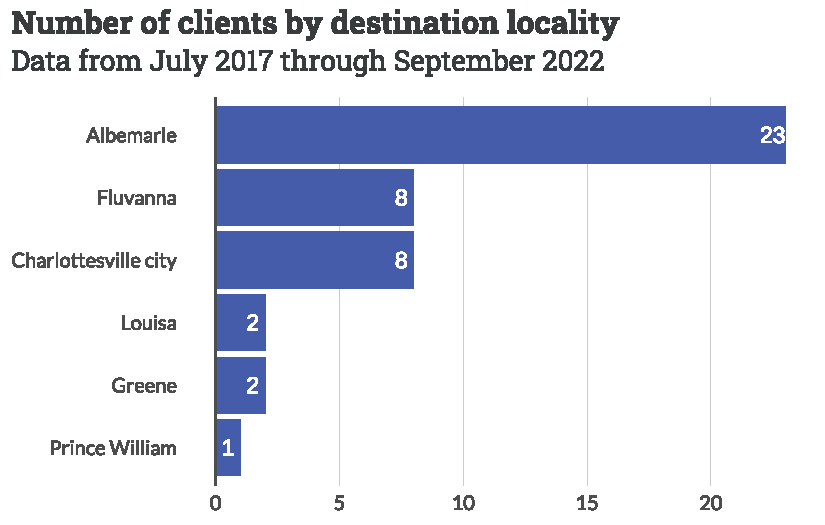
\includegraphics{piedmont_files/figure-pdf/property-locality-1.pdf}

}

\end{figure}

\hypertarget{client-moves}{%
\subsubsection{Client moves}\label{client-moves}}

Most of PHA's DPL clients moved from, moved to, or stayed in Albemarle
County or the City of Charlottesville. A similar number of clients were
originally from Albemarle (20) and Charlottesville (17), with only seven
from elsewhere. Albemarle was the most common destination (22), followed
by Charlottesville (9), and Fluvanna (8).

\begin{Shaded}
\begin{Highlighting}[]
\FunctionTok{library}\NormalTok{(ggsankey)}

\NormalTok{client\_moves }\OtherTok{\textless{}{-}} \FunctionTok{st\_drop\_geometry}\NormalTok{(clients\_sf) }\SpecialCharTok{|\textgreater{}} 
  \FunctionTok{left\_join}\NormalTok{(}\FunctionTok{st\_drop\_geometry}\NormalTok{(property\_sf), }\StringTok{"id\_pha"}\NormalTok{) }\SpecialCharTok{|\textgreater{}} 
  \FunctionTok{select}\NormalTok{(}\StringTok{"Origin"} \OtherTok{=} \StringTok{\textquotesingle{}Locality.x\textquotesingle{}}\NormalTok{, }\StringTok{"Destination"} \OtherTok{=} \StringTok{\textquotesingle{}Locality.y\textquotesingle{}}\NormalTok{) }\SpecialCharTok{|\textgreater{}} 
  \FunctionTok{mutate}\NormalTok{(}\FunctionTok{across}\NormalTok{(}\DecValTok{1}\SpecialCharTok{:}\DecValTok{2}\NormalTok{, }\SpecialCharTok{\textasciitilde{}} \FunctionTok{str\_remove\_all}\NormalTok{(.x, }\StringTok{" city"}\NormalTok{)))}

\NormalTok{client\_sankey }\OtherTok{\textless{}{-}}\NormalTok{ client\_moves }\SpecialCharTok{|\textgreater{}} 
  \FunctionTok{make\_long}\NormalTok{(Origin, Destination)}

\FunctionTok{ggplot}\NormalTok{(client\_sankey, }\FunctionTok{aes}\NormalTok{(}\AttributeTok{x =}\NormalTok{ x, }\AttributeTok{next\_x =}\NormalTok{ next\_x,}
                         \AttributeTok{node =}\NormalTok{ node, }\AttributeTok{next\_node =}\NormalTok{ next\_node,}
                         \AttributeTok{fill =}\NormalTok{ node, }\AttributeTok{label =}\NormalTok{ node)) }\SpecialCharTok{+}
  \FunctionTok{geom\_sankey}\NormalTok{(}\AttributeTok{flow\_alpha =} \FloatTok{0.75}\NormalTok{, }\AttributeTok{smooth =} \DecValTok{15}\NormalTok{) }\SpecialCharTok{+}
  \FunctionTok{geom\_sankey\_label}\NormalTok{(}\AttributeTok{fill =} \StringTok{"white"}\NormalTok{, }\AttributeTok{colour =} \StringTok{"\#383c3d"}\NormalTok{, }\AttributeTok{size =} \DecValTok{3}\NormalTok{) }\SpecialCharTok{+}
  \FunctionTok{scale\_fill\_hda}\NormalTok{(}\AttributeTok{repeat\_pal =} \ConstantTok{TRUE}\NormalTok{) }\SpecialCharTok{+}
  \FunctionTok{scale\_x\_discrete}\NormalTok{(}\AttributeTok{expand =} \FunctionTok{c}\NormalTok{(}\FloatTok{0.05}\NormalTok{, }\FloatTok{0.05}\NormalTok{), }\AttributeTok{position =} \StringTok{"top"}\NormalTok{) }\SpecialCharTok{+}
  \FunctionTok{theme\_hda}\NormalTok{() }\SpecialCharTok{+}
  \FunctionTok{theme}\NormalTok{(}\AttributeTok{axis.text.y =} \FunctionTok{element\_blank}\NormalTok{(),}
        \AttributeTok{panel.grid.major.y =} \FunctionTok{element\_blank}\NormalTok{()) }\SpecialCharTok{+}
  \FunctionTok{labs}\NormalTok{(}
    \AttributeTok{title =} \StringTok{"Origin and destination of DPL clients"}\NormalTok{,}
    \AttributeTok{subtitle =} \StringTok{"Data from July 2017 through September 2022"}
\NormalTok{  )}
\end{Highlighting}
\end{Shaded}

\begin{figure}[H]

{\centering 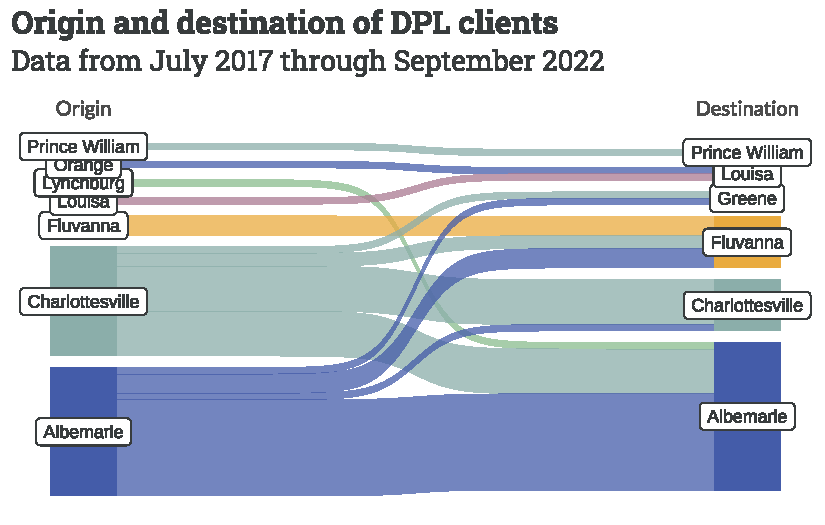
\includegraphics{piedmont_files/figure-pdf/client-moves-1.pdf}

}

\end{figure}

Among all clients from Albemarle, most stayed in the county, or to
another county. Only one moved into Charlottesville. Just seven of the
17 clients from Charlottesville stayed in the city; the same number
moved into Albemarle and the remainder to other counties.

\begin{Shaded}
\begin{Highlighting}[]
\NormalTok{client\_moves\_sum }\OtherTok{\textless{}{-}}\NormalTok{ client\_moves }\SpecialCharTok{|\textgreater{}} 
  \FunctionTok{mutate}\NormalTok{(}\AttributeTok{move =} \FunctionTok{case\_when}\NormalTok{(}
\NormalTok{    Origin }\SpecialCharTok{==}\NormalTok{ Destination }\SpecialCharTok{\textasciitilde{}} \StringTok{"Stayed"}\NormalTok{,}
    \ConstantTok{TRUE} \SpecialCharTok{\textasciitilde{}} \StringTok{"Moved"}
\NormalTok{  )) }\SpecialCharTok{|\textgreater{}} 
  \FunctionTok{mutate}\NormalTok{(}\AttributeTok{origin\_sum =} \FunctionTok{case\_when}\NormalTok{(}
\NormalTok{    Origin }\SpecialCharTok{\%in\%} \FunctionTok{c}\NormalTok{(}\StringTok{"Fluvanna"}\NormalTok{, }\StringTok{"Louisa"}\NormalTok{, }\StringTok{"Lynchburg city"}\NormalTok{, }\StringTok{"Orange"}\NormalTok{, }\StringTok{"Prince William"}\NormalTok{) }\SpecialCharTok{\textasciitilde{}} \StringTok{"From somewhere else"}\NormalTok{,}
    \ConstantTok{TRUE} \SpecialCharTok{\textasciitilde{}} \FunctionTok{str\_c}\NormalTok{(}\StringTok{"From "}\NormalTok{, Origin)}
\NormalTok{  )) }\SpecialCharTok{|\textgreater{}} 
  \FunctionTok{mutate}\NormalTok{(}\AttributeTok{destination\_sum =} \FunctionTok{case\_when}\NormalTok{(}
\NormalTok{    Destination }\SpecialCharTok{\%in\%} \FunctionTok{c}\NormalTok{(}\StringTok{"Fluvanna"}\NormalTok{, }\StringTok{"Louisa"}\NormalTok{, }\StringTok{"Greene"}\NormalTok{, }\StringTok{"Prince William"}\NormalTok{) }\SpecialCharTok{\textasciitilde{}} \StringTok{"Somewhere else"}\NormalTok{,}
    \ConstantTok{TRUE} \SpecialCharTok{\textasciitilde{}}\NormalTok{ Destination}
\NormalTok{  ))}

\FunctionTok{ggplot}\NormalTok{(client\_moves\_sum, }\FunctionTok{aes}\NormalTok{(}\AttributeTok{x =}\NormalTok{ destination\_sum, }\AttributeTok{fill =}\NormalTok{ destination\_sum)) }\SpecialCharTok{+}
  \FunctionTok{facet\_wrap}\NormalTok{(}\SpecialCharTok{\textasciitilde{}}\NormalTok{origin\_sum) }\SpecialCharTok{+}
  \FunctionTok{geom\_bar}\NormalTok{() }\SpecialCharTok{+}
  \FunctionTok{scale\_fill\_hda}\NormalTok{() }\SpecialCharTok{+}
  \FunctionTok{theme\_hda}\NormalTok{() }\SpecialCharTok{+}
  \FunctionTok{add\_zero\_line}\NormalTok{(}\StringTok{"y"}\NormalTok{) }\SpecialCharTok{+}
  \FunctionTok{theme}\NormalTok{(}\AttributeTok{legend.position =} \StringTok{"bottom"}\NormalTok{,}
        \AttributeTok{legend.title =} \FunctionTok{element\_text}\NormalTok{(),}
        \AttributeTok{axis.text.x =} \FunctionTok{element\_blank}\NormalTok{()) }\SpecialCharTok{+}
  \FunctionTok{labs}\NormalTok{(}
    \AttributeTok{title =} \StringTok{"Number of clients by origin and destination"}\NormalTok{,}
    \AttributeTok{subtitle =} \StringTok{"Data from July 2017 through September 2022"}\NormalTok{,}
    \AttributeTok{fill =} \StringTok{"Destination"}
\NormalTok{  )}
\end{Highlighting}
\end{Shaded}

\begin{figure}[H]

{\centering 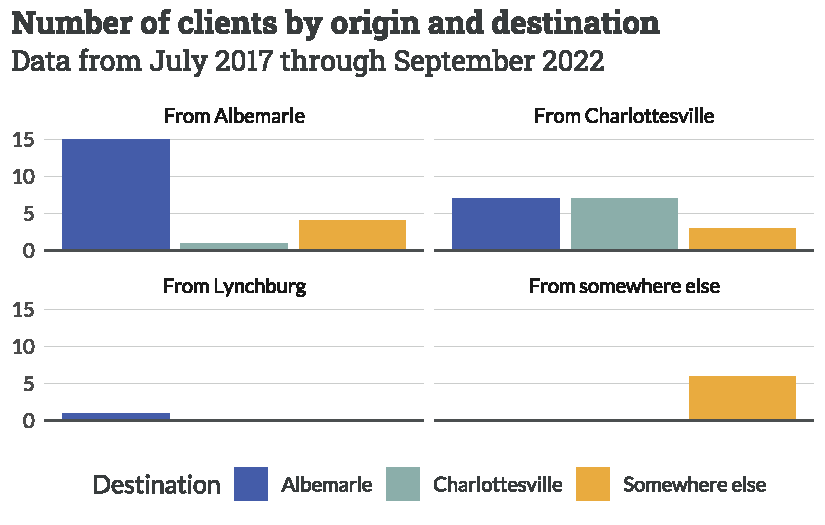
\includegraphics{piedmont_files/figure-pdf/client-moves-sum-1.pdf}

}

\end{figure}

Most white clients purchased homes in Albemarle (10), followed by
Charlottesville (5). Among the 15 Black clients, 5 bought in Albemarle,
4 in Fluvanna, 2 each in Louisa and Charlottesville, and 1 each in
Suffolk and Prince William.

\begin{Shaded}
\begin{Highlighting}[]
\FunctionTok{library}\NormalTok{(tidytext)}

\NormalTok{client\_moves\_race }\OtherTok{\textless{}{-}} \FunctionTok{st\_drop\_geometry}\NormalTok{(clients\_sf) }\SpecialCharTok{|\textgreater{}} 
  \FunctionTok{left\_join}\NormalTok{(}\FunctionTok{st\_drop\_geometry}\NormalTok{(property\_sf), }\StringTok{"id\_pha"}\NormalTok{) }\SpecialCharTok{|\textgreater{}} 
  \FunctionTok{select}\NormalTok{(}\StringTok{"race"} \OtherTok{=} \StringTok{\textquotesingle{}race.x\textquotesingle{}}\NormalTok{, }\StringTok{"Origin"} \OtherTok{=} \StringTok{\textquotesingle{}Locality.x\textquotesingle{}}\NormalTok{, }\StringTok{"Destination"} \OtherTok{=} \StringTok{\textquotesingle{}Locality.y\textquotesingle{}}\NormalTok{) }\SpecialCharTok{|\textgreater{}} 
  \FunctionTok{mutate}\NormalTok{(}\FunctionTok{across}\NormalTok{(}\DecValTok{2}\SpecialCharTok{:}\DecValTok{3}\NormalTok{, }\SpecialCharTok{\textasciitilde{}} \FunctionTok{str\_remove\_all}\NormalTok{(.x, }\StringTok{" city"}\NormalTok{))) }\SpecialCharTok{|\textgreater{}} 
  \FunctionTok{group\_by}\NormalTok{(race, Destination) }\SpecialCharTok{|\textgreater{}} 
  \FunctionTok{summarise}\NormalTok{(}\AttributeTok{n =} \FunctionTok{n}\NormalTok{()) }\SpecialCharTok{|\textgreater{}} 
  \FunctionTok{mutate}\NormalTok{(}\AttributeTok{race =} \FunctionTok{fct\_relevel}\NormalTok{(race, }\StringTok{"White"}\NormalTok{, }\StringTok{"Black"}\NormalTok{, }\StringTok{"Asian"}\NormalTok{),}
         \AttributeTok{Destination =} \FunctionTok{reorder\_within}\NormalTok{(Destination, n, race))}

\FunctionTok{ggplot}\NormalTok{(client\_moves\_race, }\FunctionTok{aes}\NormalTok{(}\AttributeTok{x =}\NormalTok{ n, }\AttributeTok{y =}\NormalTok{ Destination, }\AttributeTok{fill =}\NormalTok{ race)) }\SpecialCharTok{+}
  \FunctionTok{facet\_grid}\NormalTok{(}\AttributeTok{rows =} \FunctionTok{vars}\NormalTok{(}\FunctionTok{fct\_relevel}\NormalTok{(race, }\StringTok{"White"}\NormalTok{, }\StringTok{"Black"}\NormalTok{, }\StringTok{"Asian"}\NormalTok{)), }\AttributeTok{scales =} \StringTok{"free\_y"}\NormalTok{, }\AttributeTok{space =} \StringTok{"free\_y"}\NormalTok{, }\AttributeTok{switch =} \StringTok{"y"}\NormalTok{) }\SpecialCharTok{+}
  \FunctionTok{geom\_col}\NormalTok{() }\SpecialCharTok{+}
  \FunctionTok{scale\_x\_continuous}\NormalTok{(}
    \AttributeTok{breaks =} \FunctionTok{seq}\NormalTok{(}\DecValTok{0}\NormalTok{, }\DecValTok{10}\NormalTok{, }\DecValTok{2}\NormalTok{),}
    \AttributeTok{labels =} \FunctionTok{label\_number}\NormalTok{(}\AttributeTok{accuracy =} \DecValTok{1}\NormalTok{),}
    \AttributeTok{expand =} \FunctionTok{c}\NormalTok{(}\FloatTok{0.01}\NormalTok{, }\FloatTok{0.05}\NormalTok{)}
\NormalTok{    ) }\SpecialCharTok{+}
  \FunctionTok{scale\_y\_reordered}\NormalTok{() }\SpecialCharTok{+}
  \FunctionTok{scale\_fill\_hda}\NormalTok{() }\SpecialCharTok{+}
  \FunctionTok{add\_zero\_line}\NormalTok{(}\StringTok{"x"}\NormalTok{) }\SpecialCharTok{+}
  \FunctionTok{theme\_hda}\NormalTok{(}\AttributeTok{flip\_gridlines =} \ConstantTok{TRUE}\NormalTok{) }\SpecialCharTok{+}
  \FunctionTok{theme}\NormalTok{(}
    \AttributeTok{strip.text.y.left =} \FunctionTok{element\_text}\NormalTok{(}\AttributeTok{angle =} \DecValTok{0}\NormalTok{, }\AttributeTok{face =} \StringTok{"bold"}\NormalTok{, }\AttributeTok{vjust =} \DecValTok{1}\NormalTok{, }\AttributeTok{hjust =} \DecValTok{0}\NormalTok{),}
    \AttributeTok{strip.placement =} \StringTok{"outside"}
\NormalTok{  ) }\SpecialCharTok{+}
  \FunctionTok{labs}\NormalTok{(}
    \AttributeTok{title =} \StringTok{"DPL client destination by race"}\NormalTok{,}
    \AttributeTok{subtitle =} \StringTok{"Data from July 2017 through September 2022"}
\NormalTok{  )}
\end{Highlighting}
\end{Shaded}

\begin{figure}[H]

{\centering 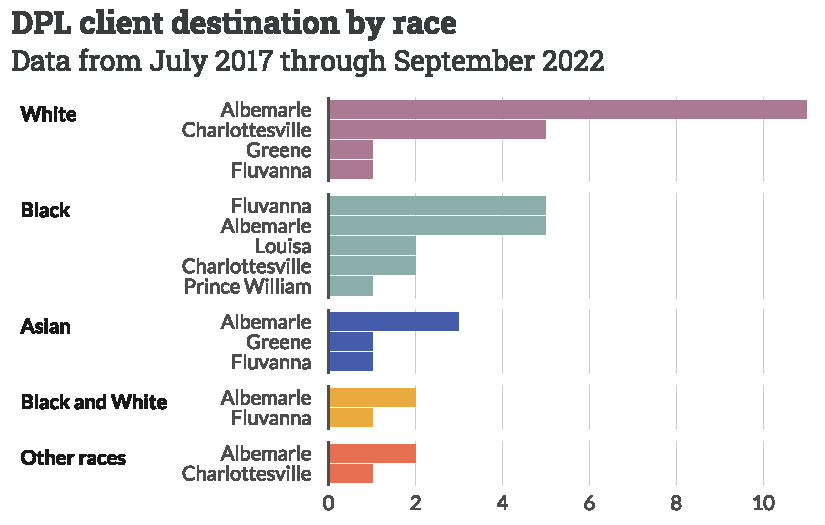
\includegraphics{piedmont_files/figure-pdf/client-moves-race-1.pdf}

}

\end{figure}

\hypertarget{housing-outcomes}{%
\subsection{Housing outcomes}\label{housing-outcomes}}

The median sales price for all clients was \$224,500, but those prices
vary significantly by program.

\begin{Shaded}
\begin{Highlighting}[]
\CommentTok{\# Summarise home sales price by program}

\NormalTok{clients\_inc\_price }\OtherTok{\textless{}{-}}\NormalTok{ clients\_all }\SpecialCharTok{|\textgreater{}} 

  \CommentTok{\# Select only id\_pha, program, income, home sales price, and race columns}
  
  \FunctionTok{select}\NormalTok{(}\DecValTok{1}\NormalTok{, }\DecValTok{2}\NormalTok{, }\DecValTok{9}\NormalTok{, }\DecValTok{10}\NormalTok{, }\DecValTok{20}\NormalTok{, }\DecValTok{21}\NormalTok{, }\DecValTok{53}\NormalTok{) }\SpecialCharTok{|\textgreater{}}
  
  \CommentTok{\# Combine DLP and SPARC incomes into one column}
  
  \FunctionTok{mutate}\NormalTok{(}\AttributeTok{income =} \FunctionTok{case\_when}\NormalTok{(}
    \SpecialCharTok{!}\FunctionTok{is.na}\NormalTok{(household\_annual\_income\_dpl) }\SpecialCharTok{\&} \SpecialCharTok{!}\FunctionTok{is.na}\NormalTok{(household\_annual\_income\_spc) }\SpecialCharTok{\textasciitilde{}}\NormalTok{ household\_annual\_income\_dpl,}
    \SpecialCharTok{!}\FunctionTok{is.na}\NormalTok{(household\_annual\_income\_dpl) }\SpecialCharTok{\&} \FunctionTok{is.na}\NormalTok{(household\_annual\_income\_spc) }\SpecialCharTok{\textasciitilde{}}\NormalTok{ household\_annual\_income\_dpl,}
    \FunctionTok{is.na}\NormalTok{(household\_annual\_income\_dpl) }\SpecialCharTok{\&} \SpecialCharTok{!}\FunctionTok{is.na}\NormalTok{(household\_annual\_income\_spc) }\SpecialCharTok{\textasciitilde{}}\NormalTok{ household\_annual\_income\_spc,}
    \ConstantTok{TRUE} \SpecialCharTok{\textasciitilde{}} \ConstantTok{NA\_real\_}
\NormalTok{  )) }\SpecialCharTok{|\textgreater{}} 

  \CommentTok{\# Combine DLP and SPARC sales prices into one column}
  
  \FunctionTok{mutate}\NormalTok{(}\AttributeTok{price =} \FunctionTok{case\_when}\NormalTok{(}
    \SpecialCharTok{!}\FunctionTok{is.na}\NormalTok{(sale\_price\_dpl) }\SpecialCharTok{\textasciitilde{}}\NormalTok{ sale\_price\_dpl,}
    \ConstantTok{TRUE} \SpecialCharTok{\textasciitilde{}}\NormalTok{ sale\_price\_spc}
\NormalTok{  ))}

\CommentTok{\# Generate table}

\NormalTok{clients\_inc\_price }\SpecialCharTok{|\textgreater{}} 
  \FunctionTok{drop\_na}\NormalTok{(price) }\SpecialCharTok{|\textgreater{}} 
  \FunctionTok{group\_by}\NormalTok{(program) }\SpecialCharTok{|\textgreater{}} 
  \FunctionTok{summarise}\NormalTok{(}\AttributeTok{n =} \FunctionTok{n}\NormalTok{(),}
            \AttributeTok{median =} \FunctionTok{median}\NormalTok{(price),}
            \AttributeTok{mean =} \FunctionTok{mean}\NormalTok{(price)) }\SpecialCharTok{|\textgreater{}} 
  \FunctionTok{mutate}\NormalTok{(}\FunctionTok{across}\NormalTok{(}\DecValTok{3}\SpecialCharTok{:}\DecValTok{4}\NormalTok{, }\SpecialCharTok{\textasciitilde{}}\NormalTok{ formattable}\SpecialCharTok{::}\FunctionTok{currency}\NormalTok{(.x, }\AttributeTok{digits =} \DecValTok{0}\NormalTok{))) }\SpecialCharTok{|\textgreater{}} 
  \FunctionTok{arrange}\NormalTok{(}\FunctionTok{desc}\NormalTok{(median)) }\SpecialCharTok{|\textgreater{}} 
  \FunctionTok{kable}\NormalTok{(}\AttributeTok{col.names =} \FunctionTok{c}\NormalTok{(}\StringTok{"Program"}\NormalTok{, }\StringTok{"Clients"}\NormalTok{, }\StringTok{"Median sales price"}\NormalTok{, }\StringTok{"Mean sales price"}\NormalTok{)) }\SpecialCharTok{|\textgreater{}} 
\NormalTok{  kableExtra}\SpecialCharTok{::}\FunctionTok{kable\_styling}\NormalTok{(}
    \AttributeTok{bootstrap\_options =} \FunctionTok{c}\NormalTok{(}\StringTok{"striped"}\NormalTok{, }\StringTok{"hover"}\NormalTok{, }\StringTok{"condensed"}\NormalTok{, }\StringTok{"responsive"}\NormalTok{)}
\NormalTok{  )}
\end{Highlighting}
\end{Shaded}

\begin{table}
\centering
\begin{tabular}{l|r|r|r}
\hline
Program & Clients & Median sales price & Mean sales price\\
\hline
Both & 8 & \$254,050 & \$241,363\\
\hline
SPARC & 86 & \$228,800 & \$226,923\\
\hline
DPL & 36 & \$184,753 & \$200,497\\
\hline
\end{tabular}
\end{table}

Home prices were lowest for DPL-only clients, with most between
\$150,000 and \$200,000. SPARC-only clients purchased homes generally
between \$200,000 and \$250,000. Clients who used both programs were
able to purchase homes at higher prices, on average, than all other
clients.

\begin{Shaded}
\begin{Highlighting}[]
\FunctionTok{ggplot}\NormalTok{(clients\_inc\_price, }\FunctionTok{aes}\NormalTok{(}\AttributeTok{x =}\NormalTok{ price, }\AttributeTok{y =}\NormalTok{ program, }\AttributeTok{fill =}\NormalTok{ program)) }\SpecialCharTok{+}
  \FunctionTok{geom\_density\_ridges}\NormalTok{(}\AttributeTok{alpha =} \FloatTok{0.9}\NormalTok{) }\SpecialCharTok{+}
  \FunctionTok{scale\_fill\_hda}\NormalTok{() }\SpecialCharTok{+}
  \FunctionTok{scale\_x\_continuous}\NormalTok{(}\AttributeTok{labels =} \FunctionTok{label\_dollar}\NormalTok{(),}
                     \AttributeTok{limits =} \FunctionTok{c}\NormalTok{(}\DecValTok{75000}\NormalTok{, }\DecValTok{350000}\NormalTok{),}
                     \AttributeTok{breaks =} \FunctionTok{c}\NormalTok{(}\DecValTok{100000}\NormalTok{, }\DecValTok{150000}\NormalTok{, }\DecValTok{200000}\NormalTok{, }\DecValTok{250000}\NormalTok{, }\DecValTok{300000}\NormalTok{)) }\SpecialCharTok{+}
  \FunctionTok{labs}\NormalTok{(}\AttributeTok{title =} \StringTok{"Client home purchase price by program"}\NormalTok{,}
       \AttributeTok{subtitle =} \StringTok{"Data from July 2017 through September 2022"}\NormalTok{) }\SpecialCharTok{+}
  \FunctionTok{theme\_hda}\NormalTok{() }\SpecialCharTok{+}
  \FunctionTok{flip\_gridlines}\NormalTok{()}
\end{Highlighting}
\end{Shaded}

\begin{figure}[H]

{\centering 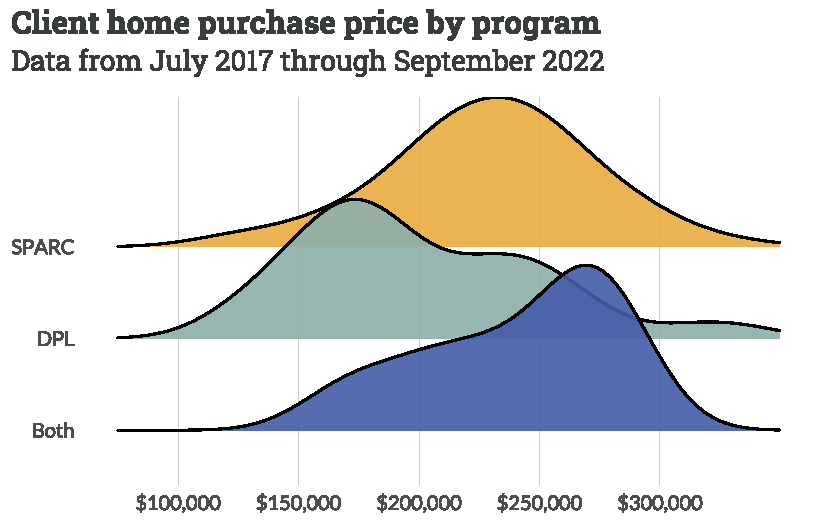
\includegraphics{piedmont_files/figure-pdf/price-plot-1.pdf}

}

\end{figure}

Average home prices also vary by race. Clients identifying as another
race have the highest average, surpassing \$250,000, although this
includes only three buyers. Clients whose records do not include their
race also have high average prices around \$227,000. These are nearly
all SPARC-only clients.

Asian and Black clients have average home prices slightly below the
average for all clients, followed by clients who are White or who are
White and Black. Those clients have average home prices well below
\$200,000.

\begin{Shaded}
\begin{Highlighting}[]
\NormalTok{clients\_price\_race }\OtherTok{\textless{}{-}}\NormalTok{ clients\_inc\_price }\SpecialCharTok{|\textgreater{}} 
  \FunctionTok{drop\_na}\NormalTok{(price) }\SpecialCharTok{|\textgreater{}} 
  \FunctionTok{group\_by}\NormalTok{(race) }\SpecialCharTok{|\textgreater{}} 
  \FunctionTok{summarise}\NormalTok{(}\AttributeTok{n =} \FunctionTok{n}\NormalTok{(),}
            \AttributeTok{Mean =} \FunctionTok{mean}\NormalTok{(price),}
            \AttributeTok{Median =} \FunctionTok{median}\NormalTok{(price)) }\SpecialCharTok{|\textgreater{}} 
  \FunctionTok{mutate}\NormalTok{(}\AttributeTok{race =} \FunctionTok{replace\_na}\NormalTok{(race, }\StringTok{"No data"}\NormalTok{)) }\SpecialCharTok{|\textgreater{}} 
  \FunctionTok{pivot\_longer}\NormalTok{(}\DecValTok{3}\SpecialCharTok{:}\DecValTok{4}\NormalTok{, }\AttributeTok{names\_to =} \StringTok{"stat"}\NormalTok{, }\AttributeTok{values\_to =} \StringTok{"value"}\NormalTok{)}

\FunctionTok{ggplot}\NormalTok{(clients\_price\_race, }\FunctionTok{aes}\NormalTok{(}\AttributeTok{x =}\NormalTok{ value, }\AttributeTok{y =} \FunctionTok{reorder}\NormalTok{(race, value),}
                               \AttributeTok{fill =}\NormalTok{ stat,}
                               \AttributeTok{label =} \FunctionTok{label\_dollar}\NormalTok{(}\AttributeTok{accuracy =} \DecValTok{1}\NormalTok{, }\AttributeTok{scale =} \FloatTok{0.001}\NormalTok{, }\AttributeTok{suffix =} \StringTok{"k"}\NormalTok{)(value))) }\SpecialCharTok{+}
  \FunctionTok{geom\_col}\NormalTok{(}\AttributeTok{position =} \StringTok{"dodge"}\NormalTok{) }\SpecialCharTok{+}
  \FunctionTok{geom\_text}\NormalTok{(}\AttributeTok{color =} \StringTok{"white"}\NormalTok{, }\AttributeTok{hjust =} \FloatTok{1.25}\NormalTok{, }\AttributeTok{position =} \FunctionTok{position\_dodge}\NormalTok{(}\FloatTok{0.9}\NormalTok{)) }\SpecialCharTok{+}
  \FunctionTok{scale\_fill\_hda}\NormalTok{() }\SpecialCharTok{+}
  \FunctionTok{scale\_x\_continuous}\NormalTok{(}\AttributeTok{labels =} \FunctionTok{label\_dollar}\NormalTok{(),}
                     \AttributeTok{breaks =} \FunctionTok{c}\NormalTok{(}\DecValTok{0}\NormalTok{, }\DecValTok{50000}\NormalTok{, }\DecValTok{100000}\NormalTok{, }\DecValTok{150000}\NormalTok{, }\DecValTok{200000}\NormalTok{, }\DecValTok{250000}\NormalTok{)) }\SpecialCharTok{+}
  \FunctionTok{labs}\NormalTok{(}\AttributeTok{title =} \StringTok{"Average client home purchase price by race"}\NormalTok{,}
       \AttributeTok{subtitle =} \StringTok{"Data from July 2017 through September 2022"}\NormalTok{) }\SpecialCharTok{+}
  \FunctionTok{theme\_hda}\NormalTok{() }\SpecialCharTok{+}
  \FunctionTok{flip\_gridlines}\NormalTok{() }\SpecialCharTok{+}
  \FunctionTok{add\_zero\_line}\NormalTok{(}\StringTok{"x"}\NormalTok{) }\SpecialCharTok{+}
  \FunctionTok{theme}\NormalTok{(}\AttributeTok{legend.position =} \StringTok{"top"}\NormalTok{) }\SpecialCharTok{+}
  \FunctionTok{guides}\NormalTok{(}\AttributeTok{fill =} \FunctionTok{guide\_legend}\NormalTok{(}\AttributeTok{reverse =} \ConstantTok{TRUE}\NormalTok{))}
\end{Highlighting}
\end{Shaded}

\begin{figure}[H]

{\centering 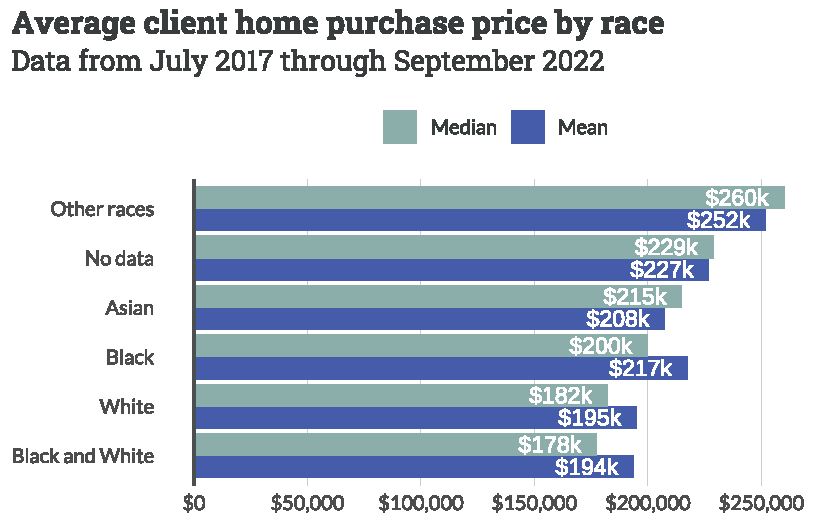
\includegraphics{piedmont_files/figure-pdf/price-race-1.pdf}

}

\end{figure}

\ldots{}

\begin{Shaded}
\begin{Highlighting}[]
\CommentTok{\# Client home attributes and price compared to neighborhood}
\CommentTok{\# Client loan products compared to region (and neighborhood, if possible)}
\end{Highlighting}
\end{Shaded}

\hypertarget{sec-home-equity}{%
\subsection{Home equity}\label{sec-home-equity}}

This section explores methods for estimating the amount of home equity
that clients have earned since the purchase of their home.

Home equity is defined as:

\[E = V - B\]

\begin{itemize}
\tightlist
\item
  \(E\) = Home equity
\item
  \(V\) = Current market value of home
\item
  \(B\) = Remaining loan balance
\end{itemize}

The data provided by PHA allows us to accurately calculate a client's
remaining loan balance. However, an accurate figure for a home's current
value would require a very recent arms-length sale or appraisal. Since
these are not available for all homes in the dataset, we will estimate
the current value with alternative data sources.

Two different methods for projecting equity will be used: the first uses
annual property assessment values, while the second uses property sales
records also collected by the local assessor.

\hypertarget{estimating-equity-via-assessments}{%
\subsubsection{Estimating equity via
assessments}\label{estimating-equity-via-assessments}}

The steps below show the process for estimating home equity for a sample
of clients in the City of Charlottesville who purchased their home in
2017, when DPL data is first available.

\textbf{Step 1: Select clients}

Select the earliest recorded DPL clients who purchased a home in the
City of Charlottesville in 2017. This gives us the longest ownership
timeframe for accruing home equity.

\begin{Shaded}
\begin{Highlighting}[]
\NormalTok{prop\_2017 }\OtherTok{\textless{}{-}}\NormalTok{ property\_sf }\SpecialCharTok{|\textgreater{}} 
  
  \CommentTok{\# Select clients with close dates in 2017}
  
  \FunctionTok{filter}\NormalTok{(}\FunctionTok{as\_date}\NormalTok{(close\_date\_dpl) }\SpecialCharTok{\textless{}} \FunctionTok{as\_date}\NormalTok{(}\StringTok{"2018{-}01{-}01"}\NormalTok{)) }\SpecialCharTok{|\textgreater{}} 
  
  \CommentTok{\# Homes purchased in Charlottesville only}
  
  \FunctionTok{filter}\NormalTok{(Locality }\SpecialCharTok{==} \StringTok{"Charlottesville city"}\NormalTok{) }\SpecialCharTok{|\textgreater{}} 
  
  \CommentTok{\# Keep only necessary columns}
  
  \FunctionTok{select}\NormalTok{(id\_pha, close\_date\_dpl, property\_street\_address, sale\_price\_dpl,}
\NormalTok{         appraised\_value, mortgage\_amount\_dpl, interest\_rate\_dpl, GEOID)}
\end{Highlighting}
\end{Shaded}

\textbf{Step 2: Assign neighborhoods}

Determine which neighborhoods the homes are in. The averages for these
neighborhoods will be used as benchmarks. Neighborhood boundaries are
the
\href{https://opendata.charlottesville.org/datasets/charlottesville::planning-neighborhood-area/about}{Planning
Neighborhood Areas} from the City of Charlottesville.

\begin{Shaded}
\begin{Highlighting}[]
\CommentTok{\# Load in Charlottesville residential parcels}

\NormalTok{cv\_parcels }\OtherTok{\textless{}{-}} \FunctionTok{read\_rds}\NormalTok{(}\StringTok{"data/cv\_parcels.rds"}\NormalTok{)}

\CommentTok{\# Load in Charlottesville neighborhood boundaries}

\NormalTok{cv\_nhoods }\OtherTok{\textless{}{-}} \FunctionTok{st\_read}\NormalTok{(}\StringTok{"data/shp/Planning\_Neighborhood\_Area.shp"}\NormalTok{, }\AttributeTok{quiet =} \ConstantTok{TRUE}\NormalTok{) }\SpecialCharTok{|\textgreater{}} 
    \FunctionTok{st\_transform}\NormalTok{(}\DecValTok{4502}\NormalTok{)}

\CommentTok{\# Spatial join with neighborhoods and parcel records}

\NormalTok{prop\_2017 }\OtherTok{\textless{}{-}}\NormalTok{ prop\_2017 }\SpecialCharTok{|\textgreater{}} 
  \FunctionTok{st\_join}\NormalTok{(cv\_nhoods) }\SpecialCharTok{|\textgreater{}} 
  \FunctionTok{st\_join}\NormalTok{(cv\_parcels)}
\end{Highlighting}
\end{Shaded}

\textbf{Step 3: Find change in neighborhood assessments}

Calculate the change in median assessed value from 2017 to 2022 for each
neighborhood. Only single-family residential parcels are included.

\begin{Shaded}
\begin{Highlighting}[]
\CommentTok{\# Spatial join all parcels to neighborhoods}

\NormalTok{cv\_parcels\_nhood }\OtherTok{\textless{}{-}}\NormalTok{ cv\_parcels }\SpecialCharTok{|\textgreater{}} 
  
  \CommentTok{\# Convert parcels to centroid points}
  
  \FunctionTok{st\_centroid}\NormalTok{() }\SpecialCharTok{|\textgreater{}} 
  
  \CommentTok{\# Spatial join}
  
  \FunctionTok{st\_join}\NormalTok{(cv\_nhoods) }\SpecialCharTok{|\textgreater{}} 
  
  \CommentTok{\# Join annual assessment data by parcel}
  
  \FunctionTok{left\_join}\NormalTok{(cv\_assess, }\AttributeTok{by =} \StringTok{"ParcelNumber"}\NormalTok{)}

\CommentTok{\# Calculate median values by year}

\NormalTok{cv\_value\_nhood }\OtherTok{\textless{}{-}}\NormalTok{ cv\_parcels\_nhood }\SpecialCharTok{|\textgreater{}} 
  
  \CommentTok{\# Drop geometry}
  
  \FunctionTok{st\_drop\_geometry}\NormalTok{() }\SpecialCharTok{|\textgreater{}} 
  
  \CommentTok{\# Group by neighborhood and year}
  
  \FunctionTok{group\_by}\NormalTok{(NAME, TaxYear) }\SpecialCharTok{|\textgreater{}} 
  
  \CommentTok{\# Calculate groupwise median}
  
  \FunctionTok{summarise}\NormalTok{(}\AttributeTok{assessment =} \FunctionTok{median}\NormalTok{(TotalValue)) }\SpecialCharTok{|\textgreater{}} 
  
  \CommentTok{\# Filter to neighborhoods where homes are}
  
  \FunctionTok{filter}\NormalTok{(NAME }\SpecialCharTok{\%in\%} \FunctionTok{c}\NormalTok{(}\StringTok{"The Meadows"}\NormalTok{, }\StringTok{"Fifeville"}\NormalTok{)) }\SpecialCharTok{|\textgreater{}} 
  
  \CommentTok{\# Add field to mark values as neighborhood average}
  
  \FunctionTok{mutate}\NormalTok{(}\AttributeTok{value =} \StringTok{"Neighborhood average"}\NormalTok{)}
\end{Highlighting}
\end{Shaded}

\textbf{Step 4: Compare change in client and neighborhood assessments}

Calculate the percent change in assessed value for client homes and
their respective neighborhoods.

\begin{Shaded}
\begin{Highlighting}[]
\CommentTok{\# Combine percent change in assessments for homes and neighborhoods}

\NormalTok{prop\_assess }\OtherTok{\textless{}{-}}\NormalTok{ prop\_2017 }\SpecialCharTok{|\textgreater{}} 
  
  \CommentTok{\# Drop geometry}
  
  \FunctionTok{st\_drop\_geometry}\NormalTok{() }\SpecialCharTok{|\textgreater{}} 
  
  \CommentTok{\# Join annual assessment data by parcel}
  
  \FunctionTok{left\_join}\NormalTok{(cv\_assess, }\AttributeTok{by =} \StringTok{"ParcelNumber"}\NormalTok{) }\SpecialCharTok{|\textgreater{}} 
  
  \CommentTok{\# Keep only necessary columns}
  
  \FunctionTok{select}\NormalTok{(NAME, TaxYear, }\AttributeTok{assessment =}\NormalTok{ TotalValue) }\SpecialCharTok{|\textgreater{}}
  
  \CommentTok{\# Add field to mark values as client home}
  
  \FunctionTok{mutate}\NormalTok{(}\AttributeTok{value =} \StringTok{"Client home"}\NormalTok{) }\SpecialCharTok{|\textgreater{}} 
  
  \CommentTok{\# Add neighborhood values}
  
  \FunctionTok{bind\_rows}\NormalTok{(cv\_value\_nhood) }\SpecialCharTok{|\textgreater{}} 
  
  \CommentTok{\# Group by value designation and neighborhood}
  
  \FunctionTok{group\_by}\NormalTok{(value, NAME) }\SpecialCharTok{|\textgreater{}} 
  
  \CommentTok{\# Arrange ascending by year}
  
  \FunctionTok{arrange}\NormalTok{(TaxYear) }\SpecialCharTok{|\textgreater{}} 
  
  \CommentTok{\# Calculate cumulative percent change}
  
  \FunctionTok{mutate}\NormalTok{(}\AttributeTok{chg =}\NormalTok{ assessment }\SpecialCharTok{{-}} \FunctionTok{first}\NormalTok{(assessment),}
         \AttributeTok{pct\_chg =}\NormalTok{ chg }\SpecialCharTok{/} \FunctionTok{first}\NormalTok{(assessment))}
\end{Highlighting}
\end{Shaded}

Following the methods above leaves us with two homes within the City of
Charlottesville that DPL clients purchased in 2017. These homes are
located on the following blocks and neighborhoods.

\begin{itemize}
\tightlist
\item
  2300 block of North Berkshire Road (Fifeville)
\item
  800 block of Orangedale Avenue (The Meadows)
\end{itemize}

Exact addresses are omitted from this narrative for privacy.

The chart below demonstrates how we can compare the change in assessed
value for homes purchased by clients to the average change observed in
their respective neighborhoods.

\begin{Shaded}
\begin{Highlighting}[]
\FunctionTok{ggplot}\NormalTok{(prop\_assess, }\FunctionTok{aes}\NormalTok{(}\AttributeTok{x =}\NormalTok{ TaxYear, }\AttributeTok{y =}\NormalTok{ pct\_chg, }\AttributeTok{color =}\NormalTok{ value)) }\SpecialCharTok{+}
  \FunctionTok{geom\_line}\NormalTok{(}\AttributeTok{linewidth =} \DecValTok{1}\NormalTok{) }\SpecialCharTok{+}
  \FunctionTok{facet\_wrap}\NormalTok{(}\SpecialCharTok{\textasciitilde{}}\NormalTok{NAME) }\SpecialCharTok{+}
  \FunctionTok{scale\_y\_continuous}\NormalTok{(}\AttributeTok{labels =} \FunctionTok{label\_percent}\NormalTok{()) }\SpecialCharTok{+}
  \FunctionTok{scale\_color\_hda}\NormalTok{() }\SpecialCharTok{+}
  \FunctionTok{theme\_hda}\NormalTok{() }\SpecialCharTok{+}
  \FunctionTok{theme}\NormalTok{(}\AttributeTok{legend.position =} \StringTok{"top"}\NormalTok{,}
        \AttributeTok{axis.text.x =} \FunctionTok{element\_text}\NormalTok{(}\AttributeTok{angle =} \DecValTok{90}\NormalTok{)) }\SpecialCharTok{+}
  \FunctionTok{add\_zero\_line}\NormalTok{(}\StringTok{"y"}\NormalTok{) }\SpecialCharTok{+}
  \FunctionTok{labs}\NormalTok{(}\AttributeTok{title =} \StringTok{"Value of DPL client homes versus surrounding neighborhoods"}\NormalTok{,}
       \AttributeTok{subtitle =} \StringTok{"Percent change in assessed value from 2017 to 2022"}\NormalTok{,}
       \AttributeTok{caption =} \StringTok{"**Notes:** Homes sold to clients in 2017. Neighborhood average derived from median value of all single{-}family residential properties."}\NormalTok{)}
\end{Highlighting}
\end{Shaded}

\begin{figure}[H]

{\centering 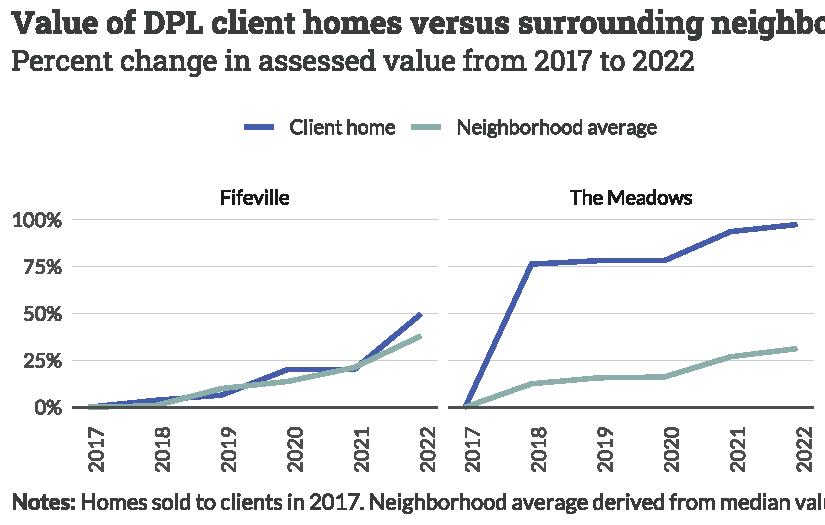
\includegraphics{piedmont_files/figure-pdf/equity-assess-plot-1.pdf}

}

\end{figure}

The plot on the left shows a client's home they purchased in Fifeville
in 2017 increasing in total assessed value by almost 50 percent by 2022,
compared to a neighborhood average increase of 38 percent.

The plot on the right shows the same for a home purchased by a client in
The Meadows. In this case, the assessed value of the client's home
almost doubled (76 percent) in the first year following their closing,
likely due to the city assessor making a major adjustment following the
sale of this home. (It was assessed for \$104,500 in 2017, but sold for
\$178,700.) Since 2018, the home's value has increased in close pace
with its surrounding neighborhood.

\begin{Shaded}
\begin{Highlighting}[]
\NormalTok{prop\_assess\_tbl }\OtherTok{\textless{}{-}}\NormalTok{ prop\_assess }\SpecialCharTok{|\textgreater{}} 
  \FunctionTok{filter}\NormalTok{(TaxYear }\SpecialCharTok{\%in\%} \FunctionTok{c}\NormalTok{(}\DecValTok{2017}\NormalTok{, }\DecValTok{2022}\NormalTok{)) }\SpecialCharTok{|\textgreater{}} 
  \FunctionTok{select}\NormalTok{(}\DecValTok{1}\NormalTok{, }\DecValTok{4}\NormalTok{, }\DecValTok{2}\NormalTok{, }\DecValTok{3}\NormalTok{, }\DecValTok{6}\NormalTok{) }\SpecialCharTok{|\textgreater{}} 
  \FunctionTok{pivot\_longer}\NormalTok{(}\AttributeTok{cols =} \DecValTok{4}\SpecialCharTok{:}\DecValTok{5}\NormalTok{, }\AttributeTok{names\_to =} \StringTok{"data"}\NormalTok{, }\AttributeTok{values\_to =} \StringTok{"x"}\NormalTok{) }\SpecialCharTok{|\textgreater{}} 
  \FunctionTok{pivot\_wider}\NormalTok{(}\AttributeTok{names\_from =}\NormalTok{ TaxYear,}
              \AttributeTok{values\_from =}\NormalTok{ x) }\SpecialCharTok{|\textgreater{}} 
  \FunctionTok{pivot\_wider}\NormalTok{(}\AttributeTok{names\_from =}\NormalTok{ data,}
              \AttributeTok{values\_from =} \StringTok{\textquotesingle{}2022\textquotesingle{}}\NormalTok{) }\SpecialCharTok{|\textgreater{}} 
  \FunctionTok{rename}\NormalTok{(}\AttributeTok{assessment17 =} \StringTok{\textquotesingle{}2017\textquotesingle{}}\NormalTok{, }\AttributeTok{assessment22 =}\NormalTok{ assessment) }\SpecialCharTok{|\textgreater{}} 
  \FunctionTok{group\_by}\NormalTok{(NAME, value) }\SpecialCharTok{|\textgreater{}} 
  \FunctionTok{mutate}\NormalTok{(}\FunctionTok{across}\NormalTok{(}\FunctionTok{where}\NormalTok{(is.double), }\SpecialCharTok{\textasciitilde{}} \FunctionTok{replace\_na}\NormalTok{(.x, }\DecValTok{0}\NormalTok{))) }\SpecialCharTok{|\textgreater{}} 
  \FunctionTok{summarise}\NormalTok{(}\FunctionTok{across}\NormalTok{(}\FunctionTok{where}\NormalTok{(is.double), }\SpecialCharTok{\textasciitilde{}} \FunctionTok{sum}\NormalTok{(.x))) }\SpecialCharTok{|\textgreater{}} 
  \FunctionTok{ungroup}\NormalTok{()}

\NormalTok{prop\_assess\_tbl }\SpecialCharTok{|\textgreater{}} 
  \FunctionTok{mutate}\NormalTok{(}\FunctionTok{across}\NormalTok{(}\DecValTok{3}\SpecialCharTok{:}\DecValTok{4}\NormalTok{, }\SpecialCharTok{\textasciitilde{}}\NormalTok{ formattable}\SpecialCharTok{::}\FunctionTok{currency}\NormalTok{(.x, }\AttributeTok{digits =} \DecValTok{0}\NormalTok{)),}
         \AttributeTok{pct\_chg =}\NormalTok{ formattable}\SpecialCharTok{::}\FunctionTok{percent}\NormalTok{(pct\_chg, }\AttributeTok{digits =} \DecValTok{1}\NormalTok{)) }\SpecialCharTok{|\textgreater{}}
  \FunctionTok{kable}\NormalTok{(}\AttributeTok{col.names =} \FunctionTok{c}\NormalTok{(}\StringTok{"Neighborhood"}\NormalTok{, }\StringTok{"Measure"}\NormalTok{, }\StringTok{"2017 assessment"}\NormalTok{, }\StringTok{"2022 assessment"}\NormalTok{, }\StringTok{"Change"}\NormalTok{),}
        \AttributeTok{align =} \StringTok{"llccc"}\NormalTok{,}
        \AttributeTok{escape =}\NormalTok{ F) }\SpecialCharTok{|\textgreater{}} 
\NormalTok{  kableExtra}\SpecialCharTok{::}\FunctionTok{kable\_styling}\NormalTok{(}
   \AttributeTok{bootstrap\_options =} \FunctionTok{c}\NormalTok{(}\StringTok{"hover"}\NormalTok{, }\StringTok{"condensed"}\NormalTok{, }\StringTok{"responsive"}\NormalTok{, }\StringTok{"striped"}\NormalTok{),}
   \AttributeTok{font\_size =} \DecValTok{14}
\NormalTok{  ) }\SpecialCharTok{|\textgreater{}} 
\NormalTok{  kableExtra}\SpecialCharTok{::}\FunctionTok{collapse\_rows}\NormalTok{(}\DecValTok{1}\NormalTok{, }\AttributeTok{valign =} \StringTok{"top"}\NormalTok{)}
\end{Highlighting}
\end{Shaded}

\hypertarget{tbl-assess}{}
\begin{table}
\caption{\label{tbl-assess}Change in assessed values for DPL client homes versus surrounding
neighborhoods }\tabularnewline

\centering\begingroup\fontsize{14}{16}\selectfont

\begin{tabular}{l|l|c|c|c}
\hline
Neighborhood & Measure & 2017 assessment & 2022 assessment & Change\\
\hline
 & Client home & $117,700 & $176,100 & 49.6%\\
\cline{2-5}
\multirow[t]{-2}{*}{\raggedright\arraybackslash Fifeville} & Neighborhood average & $191,300 & $263,950 & 38.0%\\
\cline{1-5}
 & Client home & $104,500 & $206,400 & 97.5%\\
\cline{2-5}
\multirow[t]{-2}{*}{\raggedright\arraybackslash The Meadows} & Neighborhood average & $250,800 & $329,300 & 31.3%\\
\hline
\end{tabular}
\endgroup{}
\end{table}

\textbf{Step 5: Find estimated equity}

Calculate the estimated equity for homeowners using average neighborhood
assessment increases as the benchmark.

Here, we apply the average percent increase by neighborhood to the each
home's original sales price. This gives us an estimated present value
from which to calculate home equity.

The following assumptions are made:

\begin{itemize}
\tightlist
\item
  Clients have a 30-year fixed rate mortgage with 360 total payments
\item
  Clients have made every mortgage payment from their closing date
  through the end of 2022
\item
  The monthly payment includes only principal and interest
\end{itemize}

\begin{Shaded}
\begin{Highlighting}[]
\CommentTok{\# Extract the percent change in average assessed value by neighborhood}

\NormalTok{nhood\_pct }\OtherTok{\textless{}{-}}\NormalTok{ prop\_assess\_tbl }\SpecialCharTok{|\textgreater{}} 
  \FunctionTok{filter}\NormalTok{(value }\SpecialCharTok{==} \StringTok{"Neighborhood average"}\NormalTok{) }\SpecialCharTok{|\textgreater{}} 
  \FunctionTok{select}\NormalTok{(}\DecValTok{1}\NormalTok{, }\DecValTok{5}\NormalTok{)}

\CommentTok{\# Run calculations to estimate equity}

\NormalTok{prop\_equity }\OtherTok{\textless{}{-}}\NormalTok{ prop\_2017 }\SpecialCharTok{|\textgreater{}} 
  
  \CommentTok{\# Drop geometry}
  
  \FunctionTok{st\_drop\_geometry}\NormalTok{() }\SpecialCharTok{|\textgreater{}} 
  
  \CommentTok{\# Join neighborhood assessment change data}
  
  \FunctionTok{left\_join}\NormalTok{(nhood\_pct, }\StringTok{"NAME"}\NormalTok{) }\SpecialCharTok{|\textgreater{}} 
  
  \CommentTok{\# Keep only necessary columns}
  
  \FunctionTok{select}\NormalTok{(}\DecValTok{2}\NormalTok{, }\DecValTok{3}\NormalTok{, }\DecValTok{4}\NormalTok{, }\DecValTok{6}\NormalTok{, }\DecValTok{7}\NormalTok{, }\DecValTok{10}\NormalTok{, }\DecValTok{21}\NormalTok{) }\SpecialCharTok{|\textgreater{}}
  
  \CommentTok{\# Calculate monthly payment (principal and interest only)}
  
  \FunctionTok{mutate}\NormalTok{(}\AttributeTok{pmt =}\NormalTok{  mortgage\_amount\_dpl}\SpecialCharTok{*}\NormalTok{((interest\_rate\_dpl}\SpecialCharTok{/}\DecValTok{12}\NormalTok{)}\SpecialCharTok{/}\NormalTok{(}\DecValTok{1}\SpecialCharTok{{-}}\NormalTok{(}\DecValTok{1}\SpecialCharTok{+}\NormalTok{(interest\_rate\_dpl}\SpecialCharTok{/}\DecValTok{12}\NormalTok{))}\SpecialCharTok{\^{}}\NormalTok{(}\SpecialCharTok{{-}}\DecValTok{360}\NormalTok{)))) }\SpecialCharTok{|\textgreater{}} 
  
  \CommentTok{\# Calculate number of months (payments) between closing and end of 2022}
  
  \FunctionTok{mutate}\NormalTok{(}\AttributeTok{months =}\NormalTok{ (}\FunctionTok{interval}\NormalTok{(close\_date\_dpl, }\FunctionTok{as\_date}\NormalTok{(}\StringTok{"2022{-}12{-}31"}\NormalTok{))) }\SpecialCharTok{\%/\%} \FunctionTok{months}\NormalTok{(}\DecValTok{1}\NormalTok{)) }\SpecialCharTok{|\textgreater{}} 
  
  \CommentTok{\# Calculate remaining loan balance}
  
  \FunctionTok{mutate}\NormalTok{(}\AttributeTok{balance =}\NormalTok{ (pmt}\SpecialCharTok{/}\NormalTok{(interest\_rate\_dpl}\SpecialCharTok{/}\DecValTok{12}\NormalTok{)) }\SpecialCharTok{*}\NormalTok{ (}\DecValTok{1} \SpecialCharTok{{-}}\NormalTok{ (}\DecValTok{1}\SpecialCharTok{/}\NormalTok{(}\DecValTok{1}\SpecialCharTok{+}\NormalTok{(interest\_rate\_dpl}\SpecialCharTok{/}\DecValTok{12}\NormalTok{))}\SpecialCharTok{\^{}}\NormalTok{(}\DecValTok{360}\SpecialCharTok{{-}}\NormalTok{months)))) }\SpecialCharTok{|\textgreater{}} 
  
  \CommentTok{\# Calculate estimated home value based on neighborhood assessment change}
  
  \FunctionTok{mutate}\NormalTok{(}\AttributeTok{est\_val =}\NormalTok{ sale\_price\_dpl }\SpecialCharTok{*}\NormalTok{ (}\DecValTok{1} \SpecialCharTok{+}\NormalTok{ pct\_chg)) }\SpecialCharTok{|\textgreater{}} 
  
  \CommentTok{\# Calculate home equity}
  
  \FunctionTok{mutate}\NormalTok{(}\AttributeTok{equity =}\NormalTok{ est\_val }\SpecialCharTok{{-}}\NormalTok{ balance)}
\end{Highlighting}
\end{Shaded}

The table below shows the inputs and results from the calculations
above.

\begin{Shaded}
\begin{Highlighting}[]
\NormalTok{prop\_equity\_table }\OtherTok{\textless{}{-}}\NormalTok{ prop\_equity }\SpecialCharTok{|\textgreater{}} 
  \FunctionTok{select}\NormalTok{(}\DecValTok{2}\NormalTok{, }\DecValTok{1}\NormalTok{, }\DecValTok{3}\NormalTok{, }\DecValTok{4}\NormalTok{, }\DecValTok{5}\NormalTok{, }\DecValTok{7}\SpecialCharTok{:}\DecValTok{12}\NormalTok{) }\SpecialCharTok{|\textgreater{}} 
  \FunctionTok{mutate}\NormalTok{(}\AttributeTok{property\_street\_address =} \FunctionTok{case\_when}\NormalTok{(}
    \FunctionTok{str\_detect}\NormalTok{(property\_street\_address, }\StringTok{"2302"}\NormalTok{) }\SpecialCharTok{\textasciitilde{}} \StringTok{"North Berkshire Rd"}\NormalTok{,}
    \ConstantTok{TRUE} \SpecialCharTok{\textasciitilde{}} \StringTok{"Orangedale Ave"}
\NormalTok{  )) }\SpecialCharTok{|\textgreater{}} 
  \FunctionTok{mutate}\NormalTok{(}
    \AttributeTok{close\_date\_dpl =} \FunctionTok{as.character}\NormalTok{(close\_date\_dpl),}
    \AttributeTok{interest\_rate\_dpl =} \FunctionTok{percent}\NormalTok{(interest\_rate\_dpl, }\AttributeTok{digits =} \DecValTok{3}\NormalTok{),}
    \AttributeTok{pct\_chg =} \FunctionTok{percent}\NormalTok{(pct\_chg, }\AttributeTok{digits =} \DecValTok{1}\NormalTok{),}
    \FunctionTok{across}\NormalTok{(}\FunctionTok{c}\NormalTok{(}\DecValTok{3}\NormalTok{,}\DecValTok{4}\NormalTok{,}\DecValTok{7}\NormalTok{,}\DecValTok{9}\SpecialCharTok{:}\DecValTok{11}\NormalTok{), }\SpecialCharTok{\textasciitilde{}} \FunctionTok{currency}\NormalTok{(.x, }\AttributeTok{digits =} \DecValTok{0}\NormalTok{)),}
\NormalTok{    ) }\SpecialCharTok{|\textgreater{}} 
  \FunctionTok{mutate}\NormalTok{(}\FunctionTok{across}\NormalTok{(}\DecValTok{3}\SpecialCharTok{:}\DecValTok{11}\NormalTok{, }\SpecialCharTok{\textasciitilde{}} \FunctionTok{as.character}\NormalTok{(.x))) }\SpecialCharTok{|\textgreater{}} 
  \FunctionTok{pivot\_longer}\NormalTok{(}\AttributeTok{cols =} \DecValTok{2}\SpecialCharTok{:}\DecValTok{11}\NormalTok{, }\AttributeTok{names\_to =} \StringTok{"name"}\NormalTok{, }\AttributeTok{values\_to =} \StringTok{"values"}\NormalTok{) }\SpecialCharTok{|\textgreater{}} 
  \FunctionTok{pivot\_wider}\NormalTok{(}\AttributeTok{names\_from =}\NormalTok{ property\_street\_address, }\AttributeTok{values\_from =} \DecValTok{3}\NormalTok{) }\SpecialCharTok{|\textgreater{}} 
  \FunctionTok{mutate}\NormalTok{(}\AttributeTok{name =} \FunctionTok{case\_when}\NormalTok{(}
\NormalTok{    name }\SpecialCharTok{==} \StringTok{"close\_date\_dpl"} \SpecialCharTok{\textasciitilde{}} \StringTok{"Close date"}\NormalTok{,}
\NormalTok{    name }\SpecialCharTok{==} \StringTok{"sale\_price\_dpl"} \SpecialCharTok{\textasciitilde{}} \StringTok{"Sales price"}\NormalTok{,}
\NormalTok{    name }\SpecialCharTok{==} \StringTok{"mortgage\_amount\_dpl"} \SpecialCharTok{\textasciitilde{}} \StringTok{"Principal"}\NormalTok{,}
\NormalTok{    name }\SpecialCharTok{==} \StringTok{"interest\_rate\_dpl"} \SpecialCharTok{\textasciitilde{}} \StringTok{"Interest rate"}\NormalTok{,}
\NormalTok{    name }\SpecialCharTok{==} \StringTok{"pct\_chg"} \SpecialCharTok{\textasciitilde{}} \StringTok{"Change in neighborhood assessment"}\NormalTok{,}
\NormalTok{    name }\SpecialCharTok{==} \StringTok{"pmt"} \SpecialCharTok{\textasciitilde{}} \StringTok{"Monthly payment"}\NormalTok{,}
\NormalTok{    name }\SpecialCharTok{==} \StringTok{"months"} \SpecialCharTok{\textasciitilde{}} \StringTok{"Payments made"}\NormalTok{,}
\NormalTok{    name }\SpecialCharTok{==} \StringTok{"balance"} \SpecialCharTok{\textasciitilde{}} \StringTok{"Remaining balance"}\NormalTok{,}
\NormalTok{    name }\SpecialCharTok{==} \StringTok{"est\_val"} \SpecialCharTok{\textasciitilde{}} \StringTok{"Estimated current home value"}\NormalTok{,}
\NormalTok{    name }\SpecialCharTok{==} \StringTok{"equity"} \SpecialCharTok{\textasciitilde{}} \StringTok{"Estimated equity"}
\NormalTok{  ))}
  
\NormalTok{prop\_equity\_table }\SpecialCharTok{|\textgreater{}} 
  \FunctionTok{kable}\NormalTok{(}\AttributeTok{col.names =} \FunctionTok{c}\NormalTok{(}\StringTok{""}\NormalTok{, }\StringTok{"North Berkshire Rd"}\NormalTok{, }\StringTok{"Orangedale Ave"}\NormalTok{),}
        \AttributeTok{align =} \StringTok{"lcc"}\NormalTok{,}
        \AttributeTok{escape =}\NormalTok{ F) }\SpecialCharTok{|\textgreater{}} 
\NormalTok{  kableExtra}\SpecialCharTok{::}\FunctionTok{kable\_styling}\NormalTok{(}
   \AttributeTok{bootstrap\_options =} \FunctionTok{c}\NormalTok{(}\StringTok{"hover"}\NormalTok{, }\StringTok{"condensed"}\NormalTok{, }\StringTok{"responsive"}\NormalTok{, }\StringTok{"striped"}\NormalTok{),}
   \AttributeTok{font\_size =} \DecValTok{14}
\NormalTok{  ) }\SpecialCharTok{|\textgreater{}} 
\NormalTok{  kableExtra}\SpecialCharTok{::}\FunctionTok{row\_spec}\NormalTok{(}\DecValTok{10}\NormalTok{, }\AttributeTok{bold =} \ConstantTok{TRUE}\NormalTok{)}
\end{Highlighting}
\end{Shaded}

\hypertarget{tbl-equity-assess}{}
\begin{table}
\caption{\label{tbl-equity-assess}Inputs and results for home equity estimates using assessment data }\tabularnewline

\centering\begingroup\fontsize{14}{16}\selectfont

\begin{tabular}{l|c|c}
\hline
 & North Berkshire Rd & Orangedale Ave\\
\hline
Close date & 2017-08-24 & 2017-12-05\\
\hline
Sales price & $178,700 & $126,000\\
\hline
Principal & $142,960 & $100,800\\
\hline
Interest rate & 4.375% & 3.750%\\
\hline
Change in neighborhood assessment & 31.3% & 38.0%\\
\hline
Monthly payment & $714 & $467\\
\hline
Payments made & 64 & 60\\
\hline
Remaining balance & $129,107 & $90,798\\
\hline
Estimated current home value & $234,633 & $173,851\\
\hline
\textbf{Estimated equity} & \textbf{$105,526} & \textbf{$83,053}\\
\hline
\end{tabular}
\endgroup{}
\end{table}

Based on these estimates, the homeowner on North Berkshire Road has
gained \$105,526 in home equity through 2022, and the homeowner on
Orangedale Ave has earned \$83,053.

\hypertarget{estimating-equity-via-sales-records}{%
\subsubsection{Estimating equity via sales
records}\label{estimating-equity-via-sales-records}}

The steps below show the process for estimating home equity with public
real estate sales data. This process also uses the two client homes
selected above.

\textbf{Step 1: Create list of relevant home sales}

Load in real estate sales records and join with parcel data, which
includes fields on house attributes. Remove all sales with a zero value
(which do not reflect a market transaction) and those before 2017.
Convert to spatial object and join with Charlottesville neighborhood
boundaries.

\begin{Shaded}
\begin{Highlighting}[]
\CommentTok{\# Load in real estate sales records from city}

\NormalTok{cv\_sales }\OtherTok{\textless{}{-}} \FunctionTok{read\_csv}\NormalTok{(}\StringTok{"data/raw/Real\_Estate\_(Sales).csv"}\NormalTok{) }\SpecialCharTok{|\textgreater{}} 
  
  \CommentTok{\# Join records with spatial parcel data}
  
  \FunctionTok{right\_join}\NormalTok{(cv\_parcels) }\SpecialCharTok{|\textgreater{}} 
  
  \CommentTok{\# Filter out all records that do not have a sales price}
  
  \FunctionTok{filter}\NormalTok{(SaleAmount }\SpecialCharTok{\textgreater{}} \DecValTok{0}\NormalTok{) }\SpecialCharTok{|\textgreater{}} 
  
  \CommentTok{\# Clean up date column}
  
  \FunctionTok{mutate}\NormalTok{(}\AttributeTok{SaleDate =} \FunctionTok{str\_sub}\NormalTok{(SaleDate, }\DecValTok{1}\NormalTok{, }\DecValTok{10}\NormalTok{),}
         \AttributeTok{SaleDate =} \FunctionTok{parse\_date\_time}\NormalTok{(SaleDate, }\StringTok{"ymd"}\NormalTok{)) }\SpecialCharTok{|\textgreater{}}
  
  \CommentTok{\# Filter only sales in 2017 and after}
  
  \FunctionTok{filter}\NormalTok{(SaleDate }\SpecialCharTok{\textgreater{}=} \StringTok{"2017{-}01{-}01"}\NormalTok{) }\SpecialCharTok{|\textgreater{}} 
  
  \CommentTok{\# Convert to spatial object using parcel geometry}
  
  \FunctionTok{st\_as\_sf}\NormalTok{() }\SpecialCharTok{|\textgreater{}} 
  
  \CommentTok{\# Join to neighborhoods}
  
  \FunctionTok{st\_join}\NormalTok{(cv\_nhoods)}
\end{Highlighting}
\end{Shaded}

\textbf{Step 2: Pull comps for client homes}

Filter the sales records to make a list of comps for each of the two
homes used in the prior section. Because of limited sales numbers over
the last five years, we cannot filter to neighborhoods. Instead, these
comps are based on sales of other homes that:

\begin{itemize}
\tightlist
\item
  Have the same number of bedrooms and full bathrooms, and
\item
  Are within 100 square feet of total livable area.
\end{itemize}

Using the code below, we are left with 144 comps for North Berkshire
Road and 203 for Orangedale Avenue. Median sale values for each list are
then summarized by year, followed by the cumulative percent change in
those values from 2017 to 2022.

\begin{Shaded}
\begin{Highlighting}[]
\CommentTok{\# N Berkshire Rd}
\CommentTok{\# 2 bed, 1 bath, 975 sqft}

\NormalTok{cv\_sales\_berkshire }\OtherTok{\textless{}{-}}\NormalTok{ cv\_sales }\SpecialCharTok{|\textgreater{}} 
  \FunctionTok{st\_drop\_geometry}\NormalTok{() }\SpecialCharTok{|\textgreater{}} 
  \FunctionTok{filter}\NormalTok{(Bedrooms }\SpecialCharTok{==} \DecValTok{2} \SpecialCharTok{\&}\NormalTok{ FullBathrooms }\SpecialCharTok{==} \DecValTok{1} \SpecialCharTok{\&}
\NormalTok{           SqFt }\SpecialCharTok{\textgreater{}=} \DecValTok{875} \SpecialCharTok{\&}\NormalTok{ SqFt }\SpecialCharTok{\textless{}=} \DecValTok{1075}\NormalTok{) }\SpecialCharTok{|\textgreater{}} 
  \FunctionTok{mutate}\NormalTok{(}\AttributeTok{SaleDate =} \FunctionTok{year}\NormalTok{(SaleDate)) }\SpecialCharTok{|\textgreater{}} 
  \FunctionTok{summarise}\NormalTok{(}\AttributeTok{median =} \FunctionTok{median}\NormalTok{(SaleAmount), }\AttributeTok{.by =}\NormalTok{ SaleDate) }\SpecialCharTok{|\textgreater{}} 
  \FunctionTok{arrange}\NormalTok{(median) }\SpecialCharTok{|\textgreater{}} 
  \FunctionTok{mutate}\NormalTok{(}\AttributeTok{chg =}\NormalTok{ median }\SpecialCharTok{{-}} \FunctionTok{first}\NormalTok{(median),}
         \AttributeTok{pct\_chg =}\NormalTok{ chg }\SpecialCharTok{/} \FunctionTok{first}\NormalTok{(median)) }\SpecialCharTok{|\textgreater{}} 
  \FunctionTok{mutate}\NormalTok{(}\AttributeTok{NAME =} \StringTok{"The Meadows"}\NormalTok{, }\AttributeTok{.before =} \DecValTok{1}\NormalTok{) }\SpecialCharTok{|\textgreater{}} 
  \FunctionTok{mutate}\NormalTok{(}\AttributeTok{home =} \StringTok{"North Berkshire Rd"}\NormalTok{, }\AttributeTok{.after =} \DecValTok{1}\NormalTok{)}

\CommentTok{\# Orangedale Ave}
\CommentTok{\# 3 bed, 1 bath, 1200 sqft}

\NormalTok{cv\_sales\_orangedale }\OtherTok{\textless{}{-}}\NormalTok{ cv\_sales }\SpecialCharTok{|\textgreater{}} 
  \FunctionTok{st\_drop\_geometry}\NormalTok{() }\SpecialCharTok{|\textgreater{}} 
  \FunctionTok{filter}\NormalTok{(Bedrooms }\SpecialCharTok{==} \DecValTok{3} \SpecialCharTok{\&}\NormalTok{ FullBathrooms }\SpecialCharTok{==} \DecValTok{1} \SpecialCharTok{\&}
\NormalTok{           SqFt }\SpecialCharTok{\textgreater{}=} \DecValTok{1100} \SpecialCharTok{\&}\NormalTok{ SqFt }\SpecialCharTok{\textless{}=} \DecValTok{1300}\NormalTok{) }\SpecialCharTok{|\textgreater{}} 
  \FunctionTok{mutate}\NormalTok{(}\AttributeTok{SaleDate =} \FunctionTok{year}\NormalTok{(SaleDate)) }\SpecialCharTok{|\textgreater{}} 
  \FunctionTok{summarise}\NormalTok{(}\AttributeTok{median =} \FunctionTok{median}\NormalTok{(SaleAmount), }\AttributeTok{.by =}\NormalTok{ SaleDate) }\SpecialCharTok{|\textgreater{}} 
  \FunctionTok{arrange}\NormalTok{(median) }\SpecialCharTok{|\textgreater{}} 
  \FunctionTok{mutate}\NormalTok{(}\AttributeTok{chg =}\NormalTok{ median }\SpecialCharTok{{-}} \FunctionTok{first}\NormalTok{(median),}
         \AttributeTok{pct\_chg =}\NormalTok{ chg }\SpecialCharTok{/} \FunctionTok{first}\NormalTok{(median)) }\SpecialCharTok{|\textgreater{}} 
  \FunctionTok{mutate}\NormalTok{(}\AttributeTok{NAME =} \StringTok{"Fifeville"}\NormalTok{, }\AttributeTok{.before =} \DecValTok{1}\NormalTok{) }\SpecialCharTok{|\textgreater{}} 
  \FunctionTok{mutate}\NormalTok{(}\AttributeTok{home =} \StringTok{"Orangedale Ave"}\NormalTok{, }\AttributeTok{.after =} \DecValTok{1}\NormalTok{)}

\CommentTok{\# Combine two property comps}

\NormalTok{cv\_sales\_comp }\OtherTok{\textless{}{-}} \FunctionTok{bind\_rows}\NormalTok{(cv\_sales\_berkshire, cv\_sales\_orangedale) }\SpecialCharTok{|\textgreater{}} 
  \FunctionTok{mutate}\NormalTok{(}\AttributeTok{pct\_chg =} \FunctionTok{case\_when}\NormalTok{(}
\NormalTok{    SaleDate }\SpecialCharTok{==} \DecValTok{2017} \SpecialCharTok{\textasciitilde{}} \ConstantTok{NA}\NormalTok{,}
    \ConstantTok{TRUE} \SpecialCharTok{\textasciitilde{}}\NormalTok{ pct\_chg}
\NormalTok{  ))}
\end{Highlighting}
\end{Shaded}

The plot below shows the annual median sales price calculated for each
set of comps from 2017 to 2022, as well as the cumulative percent
change. Prices for homes similar to the North Berkshire Road house have
risen 57 percent, and 69 percent for those similar to the Orangedale
Avenue home.

\begin{Shaded}
\begin{Highlighting}[]
\CommentTok{\# Plot median and percent change in annual comps for each home}

\FunctionTok{ggplot}\NormalTok{(cv\_sales\_comp,}
       \FunctionTok{aes}\NormalTok{(SaleDate,}
\NormalTok{           median,}
           \AttributeTok{fill =}\NormalTok{ home,}
           \AttributeTok{label =} \FunctionTok{label\_percent}\NormalTok{(}\AttributeTok{accuracy =} \DecValTok{1}\NormalTok{)(pct\_chg))) }\SpecialCharTok{+}
  \FunctionTok{geom\_col}\NormalTok{() }\SpecialCharTok{+}
  \FunctionTok{geom\_text}\NormalTok{(}\AttributeTok{vjust =} \DecValTok{2}\NormalTok{,}
            \AttributeTok{color =} \StringTok{"white"}\NormalTok{) }\SpecialCharTok{+}
  \FunctionTok{facet\_wrap}\NormalTok{(}\SpecialCharTok{\textasciitilde{}}\NormalTok{home) }\SpecialCharTok{+}
  \FunctionTok{scale\_fill\_hda}\NormalTok{() }\SpecialCharTok{+}
  \FunctionTok{scale\_color\_hda}\NormalTok{() }\SpecialCharTok{+}
  \FunctionTok{scale\_x\_continuous}\NormalTok{(}\AttributeTok{breaks =} \FunctionTok{c}\NormalTok{(}\DecValTok{2017}\SpecialCharTok{:}\DecValTok{2022}\NormalTok{)) }\SpecialCharTok{+}
  \FunctionTok{scale\_y\_continuous}\NormalTok{(}\AttributeTok{labels =} \FunctionTok{label\_dollar}\NormalTok{()) }\SpecialCharTok{+}
  \FunctionTok{theme\_hda}\NormalTok{() }\SpecialCharTok{+}
  \FunctionTok{add\_zero\_line}\NormalTok{(}\StringTok{"y"}\NormalTok{) }\SpecialCharTok{+}
  \FunctionTok{theme}\NormalTok{(}\AttributeTok{axis.text.x =} \FunctionTok{element\_text}\NormalTok{(}\AttributeTok{angle =} \DecValTok{90}\NormalTok{, }\AttributeTok{vjust =} \FloatTok{0.5}\NormalTok{)) }\SpecialCharTok{+}
  \FunctionTok{labs}\NormalTok{(}
    \AttributeTok{title =} \StringTok{"Value of comparable citywide sales to client homes"}\NormalTok{,}
    \AttributeTok{subtitle =} \StringTok{"Annual median sales price and cumulative percent change from 2017 to 2022"}\NormalTok{,}
    \AttributeTok{caption =} \StringTok{"**Notes:**\textless{}br\textgreater{}North Berkshire Rd comps: 2 bed, 1 bath, 875{-}975 sqft.\textless{}br\textgreater{}Orangedale Ave comps: 3 bed, 1 bath, 1100{-}1300 sqft."}
\NormalTok{  )}
\end{Highlighting}
\end{Shaded}

\begin{figure}[H]

{\centering 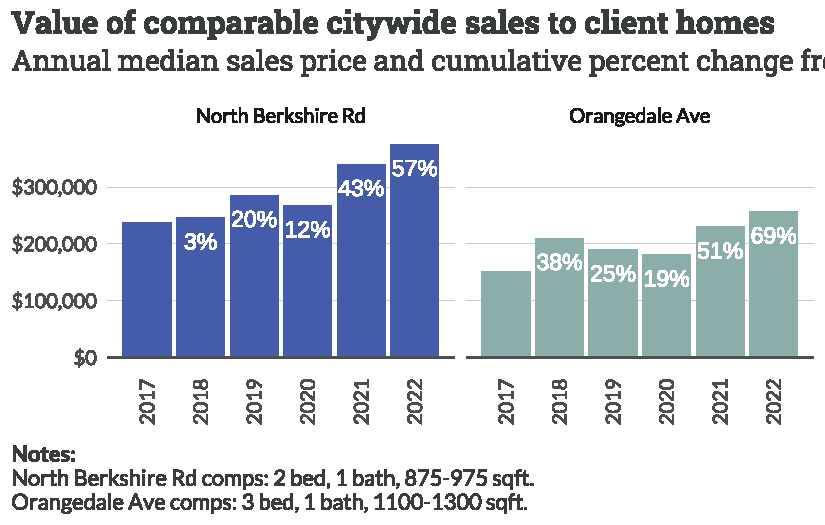
\includegraphics{piedmont_files/figure-pdf/equity-sales-plot-1.pdf}

}

\end{figure}

\textbf{Step 3: Find estimated equity}

To determine the estimated equity for each of these homes, we use the
same methods from the previous section. However, instead of applying the
percent increase in neighborhood home values, here we use the average
percent increase in sales prices for comparable homes across the whole
city.

\begin{Shaded}
\begin{Highlighting}[]
\CommentTok{\# Join with property data}

\NormalTok{prop\_comp }\OtherTok{\textless{}{-}}\NormalTok{ cv\_sales\_comp }\SpecialCharTok{|\textgreater{}} 
  \FunctionTok{filter}\NormalTok{(SaleDate }\SpecialCharTok{==} \DecValTok{2022}\NormalTok{) }\SpecialCharTok{|\textgreater{}} 
  \FunctionTok{left\_join}\NormalTok{(prop\_2017, }\AttributeTok{by =} \StringTok{"NAME"}\NormalTok{) }\SpecialCharTok{|\textgreater{}} 
  \FunctionTok{select}\NormalTok{(}\DecValTok{1}\NormalTok{, }\DecValTok{2}\NormalTok{, }\DecValTok{4}\NormalTok{, }\DecValTok{5}\NormalTok{, }\DecValTok{6}\NormalTok{, }\DecValTok{8}\NormalTok{, }\DecValTok{10}\SpecialCharTok{:}\DecValTok{13}\NormalTok{)}

\CommentTok{\# Calculate equity}

\NormalTok{comp\_equity }\OtherTok{\textless{}{-}}\NormalTok{ prop\_comp }\SpecialCharTok{|\textgreater{}} 
  \FunctionTok{mutate}\NormalTok{(}\AttributeTok{pmt =}\NormalTok{  mortgage\_amount\_dpl}\SpecialCharTok{*}\NormalTok{((interest\_rate\_dpl}\SpecialCharTok{/}\DecValTok{12}\NormalTok{)}\SpecialCharTok{/}\NormalTok{(}\DecValTok{1}\SpecialCharTok{{-}}\NormalTok{(}\DecValTok{1}\SpecialCharTok{+}\NormalTok{(interest\_rate\_dpl}\SpecialCharTok{/}\DecValTok{12}\NormalTok{))}\SpecialCharTok{\^{}}\NormalTok{(}\SpecialCharTok{{-}}\DecValTok{360}\NormalTok{)))) }\SpecialCharTok{|\textgreater{}} 
  \FunctionTok{mutate}\NormalTok{(}\AttributeTok{months =}\NormalTok{ (}\FunctionTok{interval}\NormalTok{(close\_date\_dpl, }\FunctionTok{as\_date}\NormalTok{(}\StringTok{"2022{-}12{-}31"}\NormalTok{))) }\SpecialCharTok{\%/\%} \FunctionTok{months}\NormalTok{(}\DecValTok{1}\NormalTok{)) }\SpecialCharTok{|\textgreater{}}
  \FunctionTok{mutate}\NormalTok{(}\AttributeTok{balance =}\NormalTok{ (pmt}\SpecialCharTok{/}\NormalTok{(interest\_rate\_dpl}\SpecialCharTok{/}\DecValTok{12}\NormalTok{)) }\SpecialCharTok{*}\NormalTok{ (}\DecValTok{1} \SpecialCharTok{{-}}\NormalTok{ (}\DecValTok{1}\SpecialCharTok{/}\NormalTok{(}\DecValTok{1}\SpecialCharTok{+}\NormalTok{(interest\_rate\_dpl}\SpecialCharTok{/}\DecValTok{12}\NormalTok{))}\SpecialCharTok{\^{}}\NormalTok{(}\DecValTok{360}\SpecialCharTok{{-}}\NormalTok{months)))) }\SpecialCharTok{|\textgreater{}}
  \FunctionTok{mutate}\NormalTok{(}\AttributeTok{est\_val =}\NormalTok{ sale\_price\_dpl }\SpecialCharTok{*}\NormalTok{ (}\DecValTok{1} \SpecialCharTok{+}\NormalTok{ pct\_chg)) }\SpecialCharTok{|\textgreater{}}
  \FunctionTok{mutate}\NormalTok{(}\AttributeTok{equity =}\NormalTok{ est\_val }\SpecialCharTok{{-}}\NormalTok{ balance)}
\end{Highlighting}
\end{Shaded}

The table below shows the inputs and results from the calculations
above.

\begin{Shaded}
\begin{Highlighting}[]
\NormalTok{comp\_equity\_table }\OtherTok{\textless{}{-}}\NormalTok{ comp\_equity }\SpecialCharTok{|\textgreater{}} 
  \FunctionTok{select}\NormalTok{(}\DecValTok{2}\NormalTok{, }\DecValTok{6}\NormalTok{, }\DecValTok{7}\NormalTok{, }\DecValTok{9}\NormalTok{, }\DecValTok{10}\NormalTok{, }\DecValTok{5}\NormalTok{, }\DecValTok{11}\SpecialCharTok{:}\DecValTok{15}\NormalTok{) }\SpecialCharTok{|\textgreater{}} 
  \FunctionTok{mutate}\NormalTok{(}
    \AttributeTok{close\_date\_dpl =} \FunctionTok{as.character}\NormalTok{(close\_date\_dpl),}
    \AttributeTok{interest\_rate\_dpl =} \FunctionTok{percent}\NormalTok{(interest\_rate\_dpl, }\AttributeTok{digits =} \DecValTok{3}\NormalTok{),}
    \AttributeTok{pct\_chg =} \FunctionTok{percent}\NormalTok{(pct\_chg, }\AttributeTok{digits =} \DecValTok{1}\NormalTok{),}
    \FunctionTok{across}\NormalTok{(}\FunctionTok{c}\NormalTok{(}\DecValTok{3}\NormalTok{,}\DecValTok{4}\NormalTok{,}\DecValTok{7}\NormalTok{,}\DecValTok{9}\SpecialCharTok{:}\DecValTok{11}\NormalTok{), }\SpecialCharTok{\textasciitilde{}} \FunctionTok{currency}\NormalTok{(.x, }\AttributeTok{digits =} \DecValTok{0}\NormalTok{)),}
\NormalTok{    ) }\SpecialCharTok{|\textgreater{}} 
  \FunctionTok{mutate}\NormalTok{(}\FunctionTok{across}\NormalTok{(}\DecValTok{3}\SpecialCharTok{:}\DecValTok{11}\NormalTok{, }\SpecialCharTok{\textasciitilde{}} \FunctionTok{as.character}\NormalTok{(.x))) }\SpecialCharTok{|\textgreater{}} 
  \FunctionTok{pivot\_longer}\NormalTok{(}\AttributeTok{cols =} \DecValTok{2}\SpecialCharTok{:}\DecValTok{11}\NormalTok{, }\AttributeTok{names\_to =} \StringTok{"name"}\NormalTok{, }\AttributeTok{values\_to =} \StringTok{"values"}\NormalTok{) }\SpecialCharTok{|\textgreater{}} 
  \FunctionTok{pivot\_wider}\NormalTok{(}\AttributeTok{names\_from =}\NormalTok{ home, }\AttributeTok{values\_from =} \DecValTok{3}\NormalTok{) }\SpecialCharTok{|\textgreater{}} 
  \FunctionTok{mutate}\NormalTok{(}\AttributeTok{name =} \FunctionTok{case\_when}\NormalTok{(}
\NormalTok{    name }\SpecialCharTok{==} \StringTok{"close\_date\_dpl"} \SpecialCharTok{\textasciitilde{}} \StringTok{"Close date"}\NormalTok{,}
\NormalTok{    name }\SpecialCharTok{==} \StringTok{"sale\_price\_dpl"} \SpecialCharTok{\textasciitilde{}} \StringTok{"Sales price"}\NormalTok{,}
\NormalTok{    name }\SpecialCharTok{==} \StringTok{"mortgage\_amount\_dpl"} \SpecialCharTok{\textasciitilde{}} \StringTok{"Principal"}\NormalTok{,}
\NormalTok{    name }\SpecialCharTok{==} \StringTok{"interest\_rate\_dpl"} \SpecialCharTok{\textasciitilde{}} \StringTok{"Interest rate"}\NormalTok{,}
\NormalTok{    name }\SpecialCharTok{==} \StringTok{"pct\_chg"} \SpecialCharTok{\textasciitilde{}} \StringTok{"Change in neighborhood assessment"}\NormalTok{,}
\NormalTok{    name }\SpecialCharTok{==} \StringTok{"pmt"} \SpecialCharTok{\textasciitilde{}} \StringTok{"Monthly payment"}\NormalTok{,}
\NormalTok{    name }\SpecialCharTok{==} \StringTok{"months"} \SpecialCharTok{\textasciitilde{}} \StringTok{"Payments made"}\NormalTok{,}
\NormalTok{    name }\SpecialCharTok{==} \StringTok{"balance"} \SpecialCharTok{\textasciitilde{}} \StringTok{"Remaining balance"}\NormalTok{,}
\NormalTok{    name }\SpecialCharTok{==} \StringTok{"est\_val"} \SpecialCharTok{\textasciitilde{}} \StringTok{"Estimated current home value"}\NormalTok{,}
\NormalTok{    name }\SpecialCharTok{==} \StringTok{"equity"} \SpecialCharTok{\textasciitilde{}} \StringTok{"Estimated equity"}
\NormalTok{  ))}

\NormalTok{comp\_equity\_table }\SpecialCharTok{|\textgreater{}} 
  \FunctionTok{kable}\NormalTok{(}\AttributeTok{col.names =} \FunctionTok{c}\NormalTok{(}\StringTok{""}\NormalTok{, }\StringTok{"North Berkshire Rd"}\NormalTok{, }\StringTok{"Orangedale Ave"}\NormalTok{),}
        \AttributeTok{align =} \StringTok{"lcc"}\NormalTok{,}
        \AttributeTok{escape =}\NormalTok{ F) }\SpecialCharTok{|\textgreater{}} 
\NormalTok{  kableExtra}\SpecialCharTok{::}\FunctionTok{kable\_styling}\NormalTok{(}
   \AttributeTok{bootstrap\_options =} \FunctionTok{c}\NormalTok{(}\StringTok{"hover"}\NormalTok{, }\StringTok{"condensed"}\NormalTok{, }\StringTok{"responsive"}\NormalTok{, }\StringTok{"striped"}\NormalTok{),}
   \AttributeTok{font\_size =} \DecValTok{14}
\NormalTok{  ) }\SpecialCharTok{|\textgreater{}} 
\NormalTok{  kableExtra}\SpecialCharTok{::}\FunctionTok{row\_spec}\NormalTok{(}\DecValTok{10}\NormalTok{, }\AttributeTok{bold =} \ConstantTok{TRUE}\NormalTok{)}
\end{Highlighting}
\end{Shaded}

\hypertarget{tbl-equity-sales}{}
\begin{table}
\caption{\label{tbl-equity-sales}Inputs and results for home equity estimates using home sales data }\tabularnewline

\centering\begingroup\fontsize{14}{16}\selectfont

\begin{tabular}{l|c|c}
\hline
 & North Berkshire Rd & Orangedale Ave\\
\hline
Close date & 2017-08-24 & 2017-12-05\\
\hline
Sales price & $178,700 & $126,000\\
\hline
Principal & $142,960 & $100,800\\
\hline
Interest rate & 4.375% & 3.750%\\
\hline
Change in neighborhood assessment & 57.3% & 68.8%\\
\hline
Monthly payment & $714 & $467\\
\hline
Payments made & 64 & 60\\
\hline
Remaining balance & $129,107 & $90,798\\
\hline
Estimated current home value & $281,034 & $212,729\\
\hline
\textbf{Estimated equity} & \textbf{$151,926} & \textbf{$121,931}\\
\hline
\end{tabular}
\endgroup{}
\end{table}

Based on these estimates, the homeowner on North Berkshire Road has
gained \$151,926 in home equity through 2022, and the homeowner on
Orangedale Ave has earned \$121,931.

\hypertarget{comparisons}{%
\subsubsection{Comparisons}\label{comparisons}}

These two approaches both show that the clients in these homes have
likely earned a significant amount of home equity since their purchases
in 2017. However, differences in source data and methodology produce
estimates that do vary by large amounts, even if all values are major
increases.

\begin{Shaded}
\begin{Highlighting}[]
\NormalTok{prop\_equity\_sum }\OtherTok{\textless{}{-}}\NormalTok{ prop\_equity }\SpecialCharTok{|\textgreater{}} 
  \FunctionTok{select}\NormalTok{(}\DecValTok{6}\NormalTok{, }\StringTok{"home"} \OtherTok{=} \DecValTok{2}\NormalTok{, }\DecValTok{7}\NormalTok{, }\DecValTok{11}\NormalTok{, }\DecValTok{12}\NormalTok{) }\SpecialCharTok{|\textgreater{}} 
  \FunctionTok{mutate}\NormalTok{(}\AttributeTok{method =} \StringTok{"Assessments"}\NormalTok{) }\SpecialCharTok{|\textgreater{}} 
  \FunctionTok{mutate}\NormalTok{(}\AttributeTok{home =} \FunctionTok{case\_when}\NormalTok{(}
\NormalTok{    NAME }\SpecialCharTok{==} \StringTok{"The Meadows"} \SpecialCharTok{\textasciitilde{}} \StringTok{"North Berkshire Rd"}\NormalTok{,}
    \ConstantTok{TRUE} \SpecialCharTok{\textasciitilde{}} \StringTok{"Orangedale Ave"}
\NormalTok{  ))}

\NormalTok{comp\_equity\_sum }\OtherTok{\textless{}{-}}\NormalTok{ comp\_equity }\SpecialCharTok{|\textgreater{}} 
  \FunctionTok{select}\NormalTok{(}\DecValTok{1}\NormalTok{, }\DecValTok{2}\NormalTok{,}\DecValTok{5}\NormalTok{, }\DecValTok{14}\NormalTok{, }\DecValTok{15}\NormalTok{) }\SpecialCharTok{|\textgreater{}} 
  \FunctionTok{mutate}\NormalTok{(}\AttributeTok{method =} \StringTok{"Home sales"}\NormalTok{)}

\NormalTok{equity\_sum }\OtherTok{\textless{}{-}} \FunctionTok{bind\_rows}\NormalTok{(prop\_equity\_sum, comp\_equity\_sum) }\SpecialCharTok{|\textgreater{}} 
  \FunctionTok{pivot\_longer}\NormalTok{(}\AttributeTok{cols =} \DecValTok{3}\SpecialCharTok{:}\DecValTok{5}\NormalTok{, }\AttributeTok{names\_to =} \StringTok{"type"}\NormalTok{, }\AttributeTok{values\_to =} \StringTok{"value"}\NormalTok{)}
\end{Highlighting}
\end{Shaded}

The plot below shows the differences in the estimated percent increase
of home value produced by each method (from 2017 to 2022). Using actual
market transactions (home sales) leads to much higher estimates---almost
double the results generated by the assessment data method.

\begin{Shaded}
\begin{Highlighting}[]
\NormalTok{equity\_sum }\SpecialCharTok{|\textgreater{}} 
  \FunctionTok{filter}\NormalTok{(type }\SpecialCharTok{==} \StringTok{"pct\_chg"}\NormalTok{) }\SpecialCharTok{|\textgreater{}} 
  \FunctionTok{ggplot}\NormalTok{(}\FunctionTok{aes}\NormalTok{(method, value, }\AttributeTok{fill =}\NormalTok{ method,}
             \AttributeTok{label =} \FunctionTok{label\_percent}\NormalTok{(}\AttributeTok{accuracy =} \FloatTok{0.1}\NormalTok{)(value))) }\SpecialCharTok{+}
  \FunctionTok{geom\_col}\NormalTok{() }\SpecialCharTok{+}
  \FunctionTok{geom\_text}\NormalTok{(}\AttributeTok{vjust =} \DecValTok{2}\NormalTok{,}
            \AttributeTok{color =} \StringTok{"white"}\NormalTok{) }\SpecialCharTok{+}
  \FunctionTok{facet\_wrap}\NormalTok{(}\SpecialCharTok{\textasciitilde{}}\NormalTok{home) }\SpecialCharTok{+}
  \FunctionTok{scale\_fill\_hda}\NormalTok{() }\SpecialCharTok{+}
  \FunctionTok{theme\_hda}\NormalTok{() }\SpecialCharTok{+}
  \FunctionTok{add\_zero\_line}\NormalTok{(}\StringTok{"y"}\NormalTok{) }\SpecialCharTok{+}
  \FunctionTok{theme}\NormalTok{(}\AttributeTok{axis.text.y =} \FunctionTok{element\_blank}\NormalTok{()) }\SpecialCharTok{+}
  \FunctionTok{labs}\NormalTok{(}
    \AttributeTok{title =} \StringTok{"Method comparison for estimated percent increase in home value"}\NormalTok{,}
    \AttributeTok{subtitle =} \StringTok{"Estimated percent change in home value from 2017 to 2022 by methodology"}
\NormalTok{  )}
\end{Highlighting}
\end{Shaded}

\begin{figure}[H]

{\centering 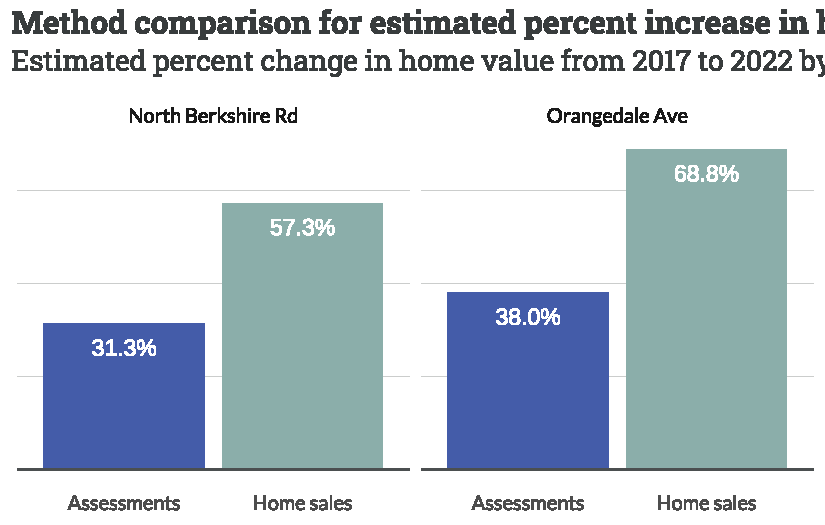
\includegraphics{piedmont_files/figure-pdf/comp-2-1.pdf}

}

\end{figure}

As a result, the estimated current home values also vary by \$40,000 to
\$50,000 depending on methodology.

\begin{Shaded}
\begin{Highlighting}[]
\NormalTok{equity\_sum }\SpecialCharTok{|\textgreater{}} 
  \FunctionTok{filter}\NormalTok{(type }\SpecialCharTok{==} \StringTok{"est\_val"}\NormalTok{) }\SpecialCharTok{|\textgreater{}} 
  \FunctionTok{ggplot}\NormalTok{(}\FunctionTok{aes}\NormalTok{(method, value, }\AttributeTok{fill =}\NormalTok{ method,}
             \AttributeTok{label =} \FunctionTok{label\_dollar}\NormalTok{()(value))) }\SpecialCharTok{+}
  \FunctionTok{geom\_col}\NormalTok{() }\SpecialCharTok{+}
  \FunctionTok{geom\_text}\NormalTok{(}\AttributeTok{vjust =} \DecValTok{2}\NormalTok{,}
            \AttributeTok{color =} \StringTok{"white"}\NormalTok{) }\SpecialCharTok{+}
  \FunctionTok{facet\_wrap}\NormalTok{(}\SpecialCharTok{\textasciitilde{}}\NormalTok{home) }\SpecialCharTok{+}
  \FunctionTok{scale\_fill\_hda}\NormalTok{() }\SpecialCharTok{+}
  \FunctionTok{theme\_hda}\NormalTok{() }\SpecialCharTok{+}
  \FunctionTok{add\_zero\_line}\NormalTok{(}\StringTok{"y"}\NormalTok{) }\SpecialCharTok{+}
  \FunctionTok{theme}\NormalTok{(}\AttributeTok{axis.text.y =} \FunctionTok{element\_blank}\NormalTok{()) }\SpecialCharTok{+}
  \FunctionTok{labs}\NormalTok{(}
    \AttributeTok{title =} \StringTok{"Method comparison for estimated current home value"}\NormalTok{,}
    \AttributeTok{subtitle =} \StringTok{"Estimated home value in 2022 by methodology"}
\NormalTok{  )}
\end{Highlighting}
\end{Shaded}

\begin{figure}[H]

{\centering 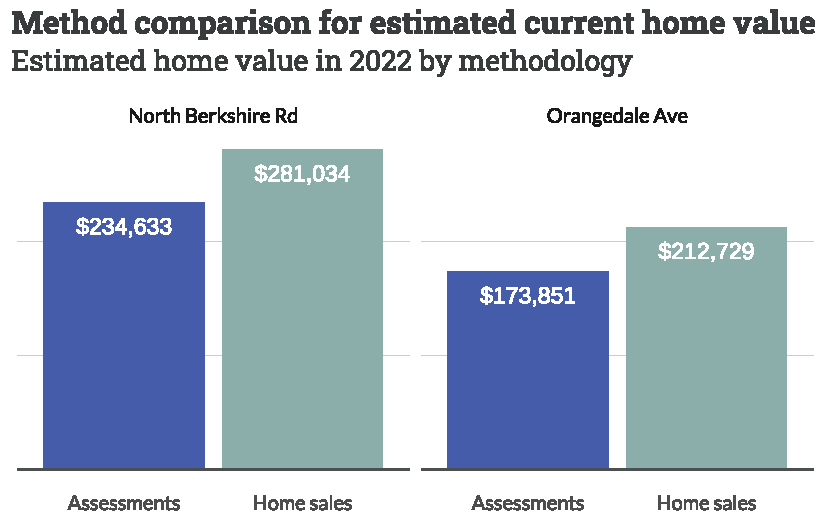
\includegraphics{piedmont_files/figure-pdf/comp-3-1.pdf}

}

\end{figure}

The estimated home values above are used to then calculate the expected
amount of home equity each homeowner has earned since their purchase.
For the North Berkshire Road home, the estimated equity ranges from
about \$105,000 to \$151,000. The latter is several thousand dollars
more than the buyer's total principal.

Equity estimates for the Orangedale Avenue home range from \$83,000 to
\$122,000. The higher estimate is just about \$4,000 less than the
buyer's original purchase price. So, while estimates do vary, both
buyers can reasonably expect significant gains in home equity relative
to their original purchase price.

\begin{Shaded}
\begin{Highlighting}[]
\NormalTok{equity\_sum }\SpecialCharTok{|\textgreater{}} 
  \FunctionTok{filter}\NormalTok{(type }\SpecialCharTok{==} \StringTok{"equity"}\NormalTok{) }\SpecialCharTok{|\textgreater{}} 
  \FunctionTok{ggplot}\NormalTok{(}\FunctionTok{aes}\NormalTok{(method, value, }\AttributeTok{fill =}\NormalTok{ method,}
             \AttributeTok{label =} \FunctionTok{label\_dollar}\NormalTok{()(value))) }\SpecialCharTok{+}
  \FunctionTok{geom\_col}\NormalTok{() }\SpecialCharTok{+}
  \FunctionTok{geom\_text}\NormalTok{(}\AttributeTok{vjust =} \DecValTok{2}\NormalTok{,}
            \AttributeTok{color =} \StringTok{"white"}\NormalTok{) }\SpecialCharTok{+}
  \FunctionTok{facet\_wrap}\NormalTok{(}\SpecialCharTok{\textasciitilde{}}\NormalTok{home) }\SpecialCharTok{+}
  \FunctionTok{scale\_fill\_hda}\NormalTok{() }\SpecialCharTok{+}
  \FunctionTok{theme\_hda}\NormalTok{() }\SpecialCharTok{+}
  \FunctionTok{add\_zero\_line}\NormalTok{(}\StringTok{"y"}\NormalTok{) }\SpecialCharTok{+}
  \FunctionTok{theme}\NormalTok{(}\AttributeTok{axis.text.y =} \FunctionTok{element\_blank}\NormalTok{()) }\SpecialCharTok{+}
  \FunctionTok{labs}\NormalTok{(}
    \AttributeTok{title =} \StringTok{"Method comparison for estimated home equity"}\NormalTok{,}
    \AttributeTok{subtitle =} \StringTok{"Estimated home equity earned from 2017 to 2022 by methodology"}
\NormalTok{  )}
\end{Highlighting}
\end{Shaded}

\begin{figure}[H]

{\centering 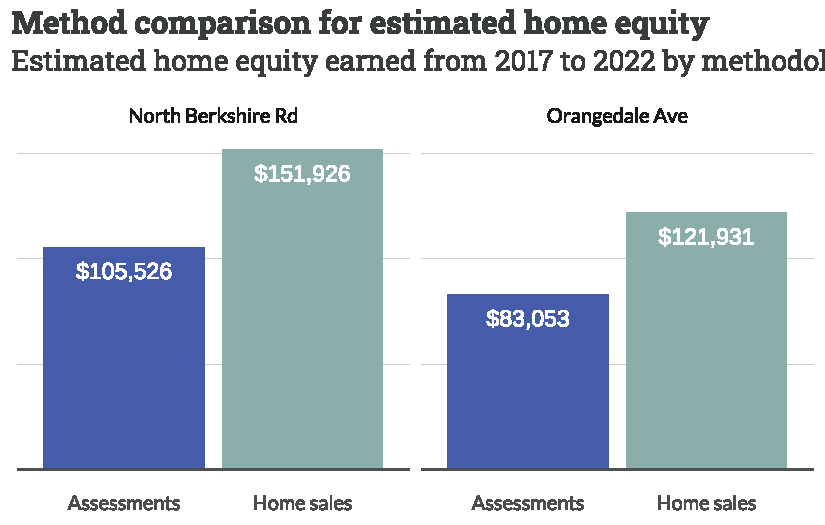
\includegraphics{piedmont_files/figure-pdf/comp-4-1.pdf}

}

\end{figure}

While many factors are at play, the major distinction between these
methods is the ability of market transactions to show much stronger home
value increases---and therefore home equity---compared to tax
assessments. Sales data are more accurately showing the accelerating
market in Charlottesville over the last five years, while the
assessments lag behind.

\hypertarget{takeaways}{%
\section{Takeaways}\label{takeaways}}

PHA has been collecting enough client data over the last five years to
generate a number of useful findings about its homebuyer programs.
Despite these achievements, expanding data integrity efforts and a host
of other next steps could help PHA develop a fuller spectrum of
analysis. Notable takeaways from this preliminary analysis are below.

Program data status:

\begin{itemize}
\tightlist
\item
  Program data is regularly collected for DPL and SPARC clients;
  however, data is inconsistent and incomplete in many places.
\item
  Despite several clients using both the DPL and SPARC programs, records
  for each are not wholly integrated and require manual joining to match
  client data.
\end{itemize}

Program findings:

\begin{itemize}
\tightlist
\item
  The number of clients served by PHA significantly accelerated in 2020
  when it began offering SPARC. Today, about two in three clients use
  SPARC only.
\item
  HOME funds from DHCD and Albemarle County HAP are by far the two most
  common down payment sources.
\item
  PHA awarded a total of \$1,242,190 in DPL assistance from July 2017 to
  September 2022. This amounted to roughly \$28,230 provided per client.
\item
  Black clients receive on average roughly \$10,000 less in down payment
  assistance than average, despite average Black home purchase prices
  totaling about \$20,000 more than those of white clients.
\item
  SPARC clients purchase higher-priced homes than DPL clients, but those
  who leverage both programs can reach prices at and above \$250,000.
\end{itemize}

Client characteristics:

\begin{itemize}
\tightlist
\item
  Although race and ethnicity data is only available for DPL records,
  overall client diversity is similar or greater than Charlottesville's
  existing demographics.
\item
  DPL clients are much more likely to earn more than most renters in
  Charlottesville, while still making significantly less than most
  homeowners.
\item
  DPL clients are more likely to move out of Charlottesville than move
  in when they purchase their new home.
\end{itemize}

Home equity gains:

\begin{itemize}
\tightlist
\item
  PHA's existing data allows for relatively robust estimates of home
  equity gains for a sample of clients.
\item
  Forecasting home equity using market sales prices results in much
  higher estimates than projecting values on annual real estate
  assessments.
\item
  Either method demonstrates \emph{significant} (six-figure) home equity
  gains for the sample clients.
\end{itemize}

\hypertarget{recommendations}{%
\section{Recommendations}\label{recommendations}}

\begin{itemize}
\tightlist
\item
  Standardize client data across programs into a single sheet and
  reconcile duplicates. The joined dataset created in Section 2.1 of
  this document is a good starting point, but other improvements should
  be explored.
\item
  Investigate the root causes for major gaps in data, such as missing
  race/ethnicity and address fields for SPARC clients.
\item
  Standardize values common data fields such as lenders, mortgage
  products, and DPL loan sources. These are discrete variables with
  known options, so entries should be consistent (i.e., avoid using both
  ``502'' and ``502 Direct Loans'').
\item
  Explore voluntary intake and exit prompts for clients. Questions
  should address knowledge gaps outside of fields that are required by
  funding sources to collect. For example, standardized recording of
  where they would prefer to buy a home can help compare aspirations to
  actual outcomes.
\end{itemize}



\end{document}
